\documentclass[10pt,a4paper]{article}
\usepackage[a4paper,margin=2.2cm]{geometry}
\usepackage{fontspec}
\usepackage{amsmath,amssymb,booktabs,longtable,array,graphicx,float,enumitem,xcolor,fancyhdr,tcolorbox}
\usepackage[colorlinks=true,linkcolor=accent,urlcolor=accent]{hyperref}
\definecolor{accent}{HTML}{1F4E79}
\sloppy\emergencystretch=3em
\setlength{\parindent}{0pt}\setlength{\parskip}{5pt}
\usepackage{titlesec}
\titleformat{\section}{\Large\bfseries\color{accent}}{}{0pt}{}
\titleformat{\subsection}{\large\bfseries\color{accent!85!black}}{}{0pt}{}
\titleformat{\subsubsection}{\normalsize\bfseries}{}{0pt}{}
\titlespacing*{\section}{0pt}{16pt}{6pt}\titlespacing*{\subsection}{0pt}{12pt}{4pt}
\pagestyle{fancy}\fancyhf{}\fancyhead[R]{\small\color{gray} Traffic Oracle $\cdot$ Team T042}\fancyfoot[C]{\small\thepage}
\renewcommand{\headrulewidth}{0pt}
\newtcolorbox{callout}{colback=orange!8,colframe=orange!60!black,boxrule=0.4pt,left=6pt,right=6pt,top=4pt,bottom=4pt,fontupper=\small}
\newtcolorbox{eqbox}{colback=black!4,colframe=black!10,boxrule=0.2pt,halign=center,fontupper=\small,left=4pt,right=4pt,top=3pt,bottom=3pt}
\begin{document}
\begin{titlepage}\centering\vspace*{3cm}
{\fontsize{40}{44}\selectfont\bfseries\color{accent} Traffic Oracle}\\[1.2cm]
{\Large Traffic speed forecasting on the METR-LA freeway network with graph attention networks, segment-level machine learning and leakage-safe hybrids --- complete technical documentation}\\[2cm]
{\large Team T042}\\[4pt]
{\large Pranav Singh \ensuremath{\cdot} Kunal \ensuremath{\cdot} Himanshu \ensuremath{\cdot} Kanchan \ensuremath{\cdot} Vaibhav}\\[4pt]
{\large Repository: github.com/\allowbreak{}Pranav-Singh-Devloper/\allowbreak{}traffic-oracle}\\[4pt]
{\large Document generated from the project's result files (results/\allowbreak{}metrics, configs, data manifest)}
\end{titlepage}
\setcounter{tocdepth}{2}\tableofcontents
\clearpage
\clearpage
\section*{1. Executive summary}\addcontentsline{toc}{section}{1. Executive summary}
This document describes the Traffic Oracle project end to end: the data, every preprocessing decision, the evaluation protocol, each model and its hyperparameters, all results with their uncertainty, the ablations, the maps, the simulated control study, the engineering set-up, and the limitations. Every number is read from the project's result files; nothing is typed by hand.

\textbf{Task.} Forecast freeway speed (mph) at 207 loop-detector sensors in Los Angeles, 5 to 60 minutes ahead (12 steps of 5 minutes), from the previous 60 minutes (12 steps). \textbf{Question.} Does information from neighbouring sensors (a road graph) improve on forecasts that use each sensor's own history, and if so, where?

{\footnotesize\renewcommand{\arraystretch}{1.15}\begin{longtable}{>{\raggedright\arraybackslash}p{0.4000\dimexpr\linewidth-8\tabcolsep\relax}>{\raggedright\arraybackslash}p{0.2000\dimexpr\linewidth-8\tabcolsep\relax}>{\raggedright\arraybackslash}p{0.2000\dimexpr\linewidth-8\tabcolsep\relax}>{\raggedright\arraybackslash}p{0.2000\dimexpr\linewidth-8\tabcolsep\relax}}
\toprule
\textbf{Model} & \textbf{MAE @ 15 min} & \textbf{MAE @ 30 min} & \textbf{MAE @ 60 min} \\
\midrule
\endhead
\bottomrule
\endlastfoot
Persistence & 3.494 & 4.198 & 5.368 \\
Historical average & 4.193 & 4.193 & 4.193 \\
Seasonal naive & 5.503 & 5.503 & 5.503 \\
XGBoost per-segment & 2.860 & 3.276 & 3.684 \\
XGBoost global (pooled) & 2.880 & 3.331 & 3.781 \\
Random Forest (multi-output) & 3.137 & 3.798 & 4.732 \\
XGBoost spatial & 2.820 & 3.258 & 3.730 \\
GRU no-graph & 2.892 \ensuremath{\pm} 0.007 & 3.313 \ensuremath{\pm} 0.013 & 3.761 \ensuremath{\pm} 0.036 \\
STGAT & 2.901 \ensuremath{\pm} 0.011 & 3.276 \ensuremath{\pm} 0.021 & 3.666 \ensuremath{\pm} 0.022 \\
Hybrid: residual & 2.820 \ensuremath{\pm} 0.005 & 3.219 \ensuremath{\pm} 0.002 & 3.647 \ensuremath{\pm} 0.009 \\
Hybrid: gating & 2.836 \ensuremath{\pm} 0.005 & 3.233 \ensuremath{\pm} 0.012 & 3.607 \ensuremath{\pm} 0.018 \\
Hybrid: average & 2.840 \ensuremath{\pm} 0.005 & 3.246 \ensuremath{\pm} 0.010 & 3.640 \ensuremath{\pm} 0.018 \\
\end{longtable}}
{\footnotesize\itshape Table 1. Headline test-set results (masked MAE in mph; \ensuremath{\pm} is the standard deviation over 3 seeds for deep models).}\par\medskip

\begin{itemize}[nosep,leftmargin=*]
\item Every learned model beats persistence. Persistence MAE grows from 3.494 to 5.368 mph between 15 and 60 minutes.
\item The best models are hybrids: the residual hybrid at 15 and 30 minutes (2.820 and 3.219 mph) and the gated hybrid at 60 minutes (3.607 mph).
\item STGAT (graph attention) equals the no-graph GRU at 15 minutes (2.901 vs 2.892) and beats it clearly only at 60 minutes (3.666 vs 3.761).
\item Hand-made neighbour features help XGBoost consistently, most at peaks and in congestion, but the gain does not grow with horizon.
\item In reduced-budget ablations the road graph was not shown to beat a no-neighbour graph; node embeddings and calendar features mattered most.
\item In an offline ramp-metering simulation, metering cut mainline congestion but forecasts did not reduce total time spent.
\end{itemize}

\clearpage
\section*{2. Problem, hypothesis and scope}\addcontentsline{toc}{section}{2. Problem, hypothesis and scope}
Congestion on freeways is not local: a jam forms at a bottleneck and its tail moves upstream (a shockwave), so downstream sensors carry information about an upstream sensor's near future. A model that sees only a sensor's own history must infer this indirectly; a graph model can read neighbouring sensors directly.

\textbf{Hypothesis.} Graph-aware models improve accuracy over per-segment models, mostly at longer horizons and during peak periods, when propagation effects dominate.

\textbf{Two phases.} Phase 1 (machine learning): exploratory analysis, naive baselines, XGBoost per sensor and pooled, a multi-output Random Forest, and XGBoost with hand-engineered neighbour features (the bridge experiment). Phase 2 (deep learning): a spatio-temporal graph attention network (STGAT), a no-graph GRU ablation, a residual hybrid and a gated hybrid that combine XGBoost with the graph model, ablations, maps, and an optional simulated ramp-metering experiment.

\begin{callout}Control is simulation only. Every control result in this document comes from an offline simulation on a synthetic network. It demonstrates how forecasts could inform a control policy; no live or real-world traffic control is performed or claimed.\end{callout}

\clearpage
\section*{Theory primer (read this first)}\addcontentsline{toc}{section}{Theory primer (read this first)}
The concepts every team member must be able to explain, in the order they appear in the pipeline. Each part ends with likely viva questions.

\subsection*{Chronological splits}\addcontentsline{toc}{subsection}{Chronological splits}
\textbf{Owner:} Kanchan

\subsubsection*{Idea}\addcontentsline{toc}{subsubsection}{Idea}
Traffic speed is strongly autocorrelated and we slide windows with stride 1, so neighboring samples share almost all of their inputs and targets. A random train/\allowbreak{}test split puts near-copies of test samples in training: the model is rewarded for memorising the immediate past, and the measured error is far lower than what it would achieve on genuinely new days.

\subsubsection*{Our protocol (strict)}\addcontentsline{toc}{subsubsection}{Our protocol (strict)}
\begin{itemize}[nosep,leftmargin=*]
\item Split the \textbf{timestamp axis}: first 70\% train, next 10\% validation, last 20\% test (\texttt{chronological\_\allowbreak{}split}).
\item Build windows \textbf{inside} each split. Window input and target never cross a boundary, so \texttt{max(train target\_\allowbreak{}ts) < min(val input\_\allowbreak{}ts)} and \texttt{max(val target\_\allowbreak{}ts) < min(test input\_\allowbreak{}ts)} (tested).
\item Everything learned from data (scaler, time-of-day means for imputation, historical-average table, target encodings, hyperparameters) uses train (or val for tuning) only.
\end{itemize}

\subsubsection*{DCRNN protocol (literature-comparable)}\addcontentsline{toc}{subsubsection}{DCRNN protocol (literature-comparable)}
DCRNN builds all windows first, then splits the \emph{samples} 70/\allowbreak{}10/\allowbreak{}20 (23974/\allowbreak{}3425/\allowbreak{}6850 here). Windows at a boundary overlap across splits (up to 23 steps), a small leak. We use it only to compare with published numbers and label it as such.

\subsubsection*{Equations}\addcontentsline{toc}{subsubsection}{Equations}
Purged boundary: with history H and horizon F, windows whose span \texttt{[t-H+1, t+F]} is wholly inside one split are the only valid ones, so each split loses \texttt{H+F-1} anchors.

\subsubsection*{Likely viva questions}\addcontentsline{toc}{subsubsection}{Likely viva questions}
\begin{itemize}[nosep,leftmargin=*]
\item \emph{Why not k-fold cross validation?} It shuffles time; use forward-chaining (expanding window) if CV is needed (we do this for OOF predictions in the hybrid).
\item \emph{Does forward-fill leak?} No: it only looks backwards in time.
\item \emph{Why report the DCRNN protocol at all?} Comparability with published MAE tables; it is labeled.
\item \emph{What distribution shift exists between our splits?} See \texttt{docs/\allowbreak{}eda\_\allowbreak{}summary.md}: the test period has a higher outage rate.
\item \emph{Why can validation still overfit?} We pick hyperparameters and early-stop on it; test is touched once.
\end{itemize}

\subsection*{Missing data}\addcontentsline{toc}{subsection}{Missing data}
\textbf{Owner:} Kanchan

\subsubsection*{Zero is not "no traffic"}\addcontentsline{toc}{subsubsection}{Zero is not "no traffic"}
In METR-LA a speed of 0 almost always means the loop detector did not report. Treating it as a real speed teaches a model that sensors randomly crash to 0 mph.

\subsubsection*{Masking}\addcontentsline{toc}{subsubsection}{Masking}
Targets: never imputed; loss and metrics sum only over observed entries: \texttt{L = \ensuremath{\Sigma} m\ensuremath{\cdot}\ensuremath{\ell}(y,\ensuremath{\hat{y}}) /\allowbreak{} \ensuremath{\Sigma} m}. Gradients come only from real observations, and normalising by \ensuremath{\Sigma}m keeps the scale independent of the batch's missing rate. The masked loss is an unbiased estimate of the loss over observed entries if missingness is independent of the target given the inputs (an assumption we cannot fully verify: outages cluster in time).

\subsubsection*{Inputs}\addcontentsline{toc}{subsubsection}{Inputs}
Option (a, default): forward-fill up to 6 steps (30 min) using only the past, then train-only time-of-day means, plus an \texttt{is\_\allowbreak{}missing} channel. Option (b, DCRNN): leave as 0 in raw space; we set it to the train mean in scaled space (ADR-003) and rely on the \texttt{is\_\allowbreak{}missing} channel. Ablation A9 compares them.

\subsubsection*{Facts in this dataset}\addcontentsline{toc}{subsubsection}{Facts in this dataset}
See \texttt{docs/\allowbreak{}eda\_\allowbreak{}summary.md}: \textasciitilde{}8\% missing, whole-network outages exist, and the test period has more outages than train.

\subsubsection*{Likely viva questions}\addcontentsline{toc}{subsubsection}{Likely viva questions}
\begin{itemize}[nosep,leftmargin=*]
\item \emph{Why not interpolate the targets?} It would invent data and reward smoothness.
\item \emph{Why a missing flag when imputing?} The model should know the value is not real.
\item \emph{Where could masking bias results?} If outages correlate with congestion.
\end{itemize}

\subsection*{Metrics}\addcontentsline{toc}{subsection}{Metrics}
\textbf{Owner:} Himanshu

All metrics are computed in \textbf{mph}, on \textbf{observed} targets only (mask = speed > 0).

\begin{itemize}[nosep,leftmargin=*]
\item \textbf{MAE} \texttt{= \ensuremath{\Sigma} m|y\ensuremath{-}\ensuremath{\hat{y}}| /\allowbreak{} \ensuremath{\Sigma} m}: average error in mph; robust, same units as speed.
\item \textbf{RMSE} \texttt{= sqrt(\ensuremath{\Sigma} m(y\ensuremath{-}\ensuremath{\hat{y}})\ensuremath{^{2}} /\allowbreak{} \ensuremath{\Sigma} m)}: penalises large errors more; larger than MAE whenever errors vary. A big RMSE/\allowbreak{}MAE gap signals occasional big misses (e.g. missing the onset of congestion).
\item \textbf{MAPE} \texttt{= 100\ensuremath{\cdot}\ensuremath{\Sigma} m'|y\ensuremath{-}\ensuremath{\hat{y}}|/\allowbreak{}y /\allowbreak{} \ensuremath{\Sigma} m'}, \texttt{m' = m \ensuremath{\wedge} (y \ensuremath{\geq} 1 mph)}: relative error; unstable at low speeds because the denominator is small, and asymmetric (over-prediction costs more than under-prediction). Use it as secondary.
\end{itemize}

\subsubsection*{Why per horizon}\addcontentsline{toc}{subsubsection}{Why per horizon}
Error grows with horizon; a single averaged number hides where models differ. Headline horizons are 15/\allowbreak{}30/\allowbreak{}60 min (steps 3/\allowbreak{}6/\allowbreak{}12); all 12 are in \texttt{all\_\allowbreak{}metrics\_\allowbreak{}long.csv}.

\subsubsection*{Why slices}\addcontentsline{toc}{subsubsection}{Why slices}
Congestion is rare overall but frequent at peaks; averaged metrics are dominated by easy free-flow samples. We also report peak, off-peak weekday, weekend, congested (<40 mph) and free-flow.

\subsubsection*{Edge cases}\addcontentsline{toc}{subsubsection}{Edge cases}
An all-masked slice returns NaN, never 0. NaN predictions (untrained horizons) are removed from the mask.

\subsubsection*{Likely viva questions}\addcontentsline{toc}{subsubsection}{Likely viva questions}
\begin{itemize}[nosep,leftmargin=*]
\item \emph{Why masked metrics?} Zero readings are outages, counting them would reward/\allowbreak{}penalise models for nothing.
\item \emph{MAE vs RMSE choice?} Report both; MAE is our training/\allowbreak{}early-stopping metric.
\item \emph{Why not MAPE as headline?} Instability at low speed.
\item \emph{Why is historical average flat across horizons?} It ignores the current state, so its error does not depend on horizon.
\end{itemize}

\subsection*{XGBoost}\addcontentsline{toc}{subsection}{XGBoost}
\textbf{Owner:} Kunal

\subsubsection*{Model}\addcontentsline{toc}{subsubsection}{Model}
Additive trees: \texttt{\ensuremath{\hat{y}}\_\allowbreak{}i = \ensuremath{\Sigma}\_\allowbreak{}\{k=1\}\^{}K f\_\allowbreak{}k(x\_\allowbreak{}i)}, each \texttt{f\_\allowbreak{}k} a regression tree with leaf weights \texttt{w}.

\subsubsection*{Objective and second-order approximation}\addcontentsline{toc}{subsubsection}{Objective and second-order approximation}
\texttt{L = \ensuremath{\Sigma}\_\allowbreak{}i l(y\_\allowbreak{}i, \ensuremath{\hat{y}}\_\allowbreak{}i) + \ensuremath{\Sigma}\_\allowbreak{}k \ensuremath{\Omega}(f\_\allowbreak{}k)}, \texttt{\ensuremath{\Omega}(f) = \ensuremath{\gamma}T + \ensuremath{\tfrac{1}{2}}\ensuremath{\lambda}\ensuremath{\Vert}w\ensuremath{\Vert}\ensuremath{^{2}}} (T leaves). At step t, expand the loss to second order around the current prediction: \texttt{L\^{}(t) \ensuremath{\approx} \ensuremath{\Sigma}\_\allowbreak{}i [g\_\allowbreak{}i f\_\allowbreak{}t(x\_\allowbreak{}i) + \ensuremath{\tfrac{1}{2}} h\_\allowbreak{}i f\_\allowbreak{}t(x\_\allowbreak{}i)\ensuremath{^{2}}] + \ensuremath{\Omega}(f\_\allowbreak{}t)}, with \texttt{g\_\allowbreak{}i = \ensuremath{\partial}l/\allowbreak{}\ensuremath{\partial}\ensuremath{\hat{y}}}, \texttt{h\_\allowbreak{}i = \ensuremath{\partial}\ensuremath{^{2}}l/\allowbreak{}\ensuremath{\partial}\ensuremath{\hat{y}}\ensuremath{^{2}}}. For a leaf containing index set I the optimal weight is \texttt{w* = \ensuremath{-}G/\allowbreak{}(H+\ensuremath{\lambda})} (G = \ensuremath{\Sigma}g, H = \ensuremath{\Sigma}h) with score \texttt{\ensuremath{-}\ensuremath{\tfrac{1}{2}} G\ensuremath{^{2}}/\allowbreak{}(H+\ensuremath{\lambda})}.

\subsubsection*{Split gain}\addcontentsline{toc}{subsubsection}{Split gain}
\texttt{Gain = \ensuremath{\tfrac{1}{2}}[ G\_\allowbreak{}L\ensuremath{^{2}}/\allowbreak{}(H\_\allowbreak{}L+\ensuremath{\lambda}) + G\_\allowbreak{}R\ensuremath{^{2}}/\allowbreak{}(H\_\allowbreak{}R+\ensuremath{\lambda}) \ensuremath{-} (G\_\allowbreak{}L+G\_\allowbreak{}R)\ensuremath{^{2}}/\allowbreak{}(H\_\allowbreak{}L+H\_\allowbreak{}R+\ensuremath{\lambda}) ] \ensuremath{-} \ensuremath{\gamma}} A split is made only if gain > 0: \ensuremath{\gamma} is a complexity price per leaf, \ensuremath{\lambda} shrinks leaf weights.

\subsubsection*{Practical details used here}\addcontentsline{toc}{subsubsection}{Practical details used here}
\begin{itemize}[nosep,leftmargin=*]
\item \texttt{tree\_\allowbreak{}method="hist"} (histogram binning, fast), early stopping on validation MAE.
\item Objective is chosen by Optuna from squared error /\allowbreak{} absolute error /\allowbreak{} pseudo-Huber; MAE is the reported metric, and absolute error targets the conditional median.
\item \textbf{Per-segment vs global:} per-segment trains one model per sensor (207 x horizons, each \textasciitilde{}24k rows, no sharing). Global pools sensors (\textasciitilde{}5M rows) with sensor id and static features, borrowing strength across sensors but still without neighbor information.
\end{itemize}

\subsubsection*{Likely viva questions}\addcontentsline{toc}{subsubsection}{Likely viva questions}
\begin{itemize}[nosep,leftmargin=*]
\item \emph{Why second order?} Newton step gives faster, more stable fitting and a closed-form leaf weight.
\item \emph{What do \ensuremath{\lambda} and \ensuremath{\gamma} do?} \ensuremath{\lambda} shrinks leaf weights; \ensuremath{\gamma} prunes splits with small gain.
\item \emph{Difference between gain importance and SHAP?} Gain is split-based and biased toward high-cardinality/\allowbreak{}early splits; SHAP attributes each prediction consistently (we use TreeSHAP via \texttt{pred\_\allowbreak{}contribs}).
\item \emph{Why can XGBoost not model propagation?} A row only contains that sensor's own history; neighbor information must be hand-engineered (XGB-spatial).
\item \emph{Why do trees handle `speed==0`-like issues badly?} We impute inputs and add missing flags; targets are masked.
\end{itemize}

\subsection*{Random Forest}\addcontentsline{toc}{subsection}{Random Forest}
\textbf{Owner:} Vaibhav

\subsubsection*{Idea}\addcontentsline{toc}{subsubsection}{Idea}
Average many decorrelated, deep trees. Each tree is fit on a bootstrap sample (\texttt{max\_\allowbreak{}samples}) and each split considers a random subset of features (\texttt{max\_\allowbreak{}features}).

\subsubsection*{Variance reduction}\addcontentsline{toc}{subsubsection}{Variance reduction}
For B trees with variance \ensuremath{\sigma}\ensuremath{^{2}} and pairwise correlation \ensuremath{\rho}: \texttt{Var(mean) = \ensuremath{\rho}\ensuremath{\sigma}\ensuremath{^{2}} + (1\ensuremath{-}\ensuremath{\rho})\ensuremath{\sigma}\ensuremath{^{2}}/\allowbreak{}B}. Bagging shrinks the second term; feature subsampling lowers \ensuremath{\rho}, which is the floor of the variance. Bias stays about that of one deep tree.

\subsubsection*{Native multi-output}\addcontentsline{toc}{subsubsection}{Native multi-output}
\texttt{RandomForestRegressor} fits one tree per bootstrap sample for all outputs at once: a split minimises the \textbf{sum of squared errors over all 12 horizons}, so a leaf stores a 12-vector. Predictions across horizons are coherent and one model replaces 12, but the split criterion is dominated by long horizons (larger errors).

\subsubsection*{Choices here}\addcontentsline{toc}{subsubsection}{Choices here}
\begin{itemize}[nosep,leftmargin=*]
\item Pooled over sensors, rows with any missing horizon target dropped (share logged), training rows subsampled (see ADR-006) for memory/\allowbreak{}time.
\item Squared-error criterion (MAE is evaluated, so RF is not tuned for the metric directly).
\end{itemize}

\subsubsection*{Likely viva questions}\addcontentsline{toc}{subsubsection}{Likely viva questions}
\begin{itemize}[nosep,leftmargin=*]
\item \emph{Why doesn't adding trees overfit?} Variance falls monotonically with B (bias is unchanged).
\item \emph{Why max\_\allowbreak{}features < all?} Decorrelates trees (lowers \ensuremath{\rho}).
\item \emph{Why does RF extrapolate poorly?} Leaves output training-set averages, so predictions stay in the observed range.
\item \emph{Multi-output pros/\allowbreak{}cons?} Coherent horizons and speed vs. no horizon-specific tuning.
\end{itemize}

\subsection*{Graph Attention Networks (GAT)}\addcontentsline{toc}{subsection}{Graph Attention Networks (GAT)}
\textbf{Owner:} Pranav Singh

Implemented in \texttt{src/\allowbreak{}traffic/\allowbreak{}models/\allowbreak{}layers/\allowbreak{}gat\_\allowbreak{}dense.py} and tested against PyG (\texttt{tests/\allowbreak{}test\_\allowbreak{}gat\_\allowbreak{}layer.py}).

\subsubsection*{Equations (one head)}\addcontentsline{toc}{subsubsection}{Equations (one head)}
\begin{itemize}[nosep,leftmargin=*]
\item \texttt{h'\_\allowbreak{}i = W h\_\allowbreak{}i}
\item \texttt{e\_\allowbreak{}ij = LeakyReLU(a\ensuremath{^{\top}} [h'\_\allowbreak{}i \ensuremath{\Vert} h'\_\allowbreak{}j])} for \texttt{j \ensuremath{\in} N(i) \ensuremath{\cup} \{i\}}, \texttt{\ensuremath{-}\ensuremath{\infty}} otherwise
\item \texttt{\ensuremath{\alpha}\_\allowbreak{}ij = softmax\_\allowbreak{}j(e\_\allowbreak{}ij)}  (masked softmax over neighbors)
\item \texttt{h\_\allowbreak{}i\^{}out = \ensuremath{\Sigma}\_\allowbreak{}j \ensuremath{\alpha}\_\allowbreak{}ij h'\_\allowbreak{}j (+ b)}, then ELU outside the layer. K heads are concatenated (averaged in an output layer).
\end{itemize}

Splitting \texttt{a = [a\_\allowbreak{}dst; a\_\allowbreak{}src]} gives \texttt{e\_\allowbreak{}ij = a\_\allowbreak{}dst\ensuremath{^{\top}} h'\_\allowbreak{}i + a\_\allowbreak{}src\ensuremath{^{\top}} h'\_\allowbreak{}j}, which is what we compute (cheap: two dot products, then a broadcast sum).

\subsubsection*{Why dense and masked}\addcontentsline{toc}{subsubsection}{Why dense and masked}
N = 207, so an [N x N] attention matrix per head is small; masking with the adjacency (non-edges to \ensuremath{-}\ensuremath{\infty}) gives exactly the sparse softmax and batches trivially. Cost O(B\ensuremath{\cdot}K\ensuremath{\cdot}N\ensuremath{^{2}}\ensuremath{\cdot}d) vs sparse O(B\ensuremath{\cdot}K\ensuremath{\cdot}|E|\ensuremath{\cdot}d).

\subsubsection*{Direction convention}\addcontentsline{toc}{subsubsection}{Direction convention}
\texttt{adj[i, j] > 0} means node i aggregates from node j (ADR-002). PyG's \texttt{edge\_\allowbreak{}index} is (source j, target i) so the test builds it with \texttt{adj.nonzero().flip(1).T}.

\subsubsection*{GCN vs GAT vs GATv2}\addcontentsline{toc}{subsubsection}{GCN vs GAT vs GATv2}
\begin{itemize}[nosep,leftmargin=*]
\item \textbf{GCN} weights neighbors by fixed normalised adjacency (\texttt{attention="mean"} ablation): same weights for every input.
\item \textbf{GAT} learns input-dependent weights, but its attention is \emph{static} in ranking: with \texttt{a\ensuremath{^{\top}}[Wh\_\allowbreak{}i\ensuremath{\Vert}Wh\_\allowbreak{}j]} the ordering of neighbors j is the same for every query node i (the score splits into a function of i plus a function of j, so softmax over j ignores i).
\item \textbf{GATv2} moves the nonlinearity inside: \texttt{a\ensuremath{^{\top}} LeakyReLU(W[h\_\allowbreak{}i\ensuremath{\Vert}h\_\allowbreak{}j])} \ensuremath{\Rightarrow} dynamic attention (\texttt{gatv2} ablation). We compute it in checkpointed chunks because the [B,N,N,K,D] tensor is large.
\end{itemize}

\subsubsection*{Edge bias}\addcontentsline{toc}{subsubsection}{Edge bias}
\texttt{e\_\allowbreak{}ij += \ensuremath{\beta}\ensuremath{\cdot}W\_\allowbreak{}ij} adds a learnable distance prior (ablation A12).

\subsubsection*{Likely viva questions}\addcontentsline{toc}{subsubsection}{Likely viva questions}
\begin{itemize}[nosep,leftmargin=*]
\item \emph{What does the mask do?} Restricts the softmax to neighbors so non-neighbors get exactly 0 attention.
\item \emph{Why LeakyReLU?} Keeps gradients for negative scores; ELU is applied to the output.
\item \emph{Why multiple heads?} Different heads can specialise (e.g. upstream vs downstream), and averaging stabilises training.
\item \emph{What is "static attention"?} See above; GATv2 fixes it.
\item \emph{Complexity?} See above.
\item \emph{Why add self-loops?} So a node can keep its own information; also avoids all \ensuremath{-}\ensuremath{\infty} rows.
\end{itemize}

\subsection*{Spatio-temporal modeling}\addcontentsline{toc}{subsection}{Spatio-temporal modeling}
\textbf{Owner:} Pranav Singh

\subsubsection*{Shockwaves}\addcontentsline{toc}{subsubsection}{Shockwaves}
Congestion starts at a bottleneck and the jam's tail moves upstream at roughly 10--15 mph (our CTM backward wave speed w \ensuremath{\approx} 12 mph). A sensor upstream of a bottleneck will slow down minutes after downstream sensors do. A per-segment model sees only its own past and learns this only indirectly, while a graph model can read the downstream state directly.

\subsubsection*{Receptive field}\addcontentsline{toc}{subsubsection}{Receptive field}
Spatial reach = L (GAT layers) hops; temporal reach = H input steps (TCN receptive field grows with dilation: kernel 3, dilations 1, 2, 4...). A shockwave at speed w covers distance w\ensuremath{\cdot}\ensuremath{\Delta}t in time \ensuremath{\Delta}t, so the graph depth needed for horizon h grows with h. Our evidence: correlation decays with graph distance (EDA fig. 6), but directional lags are only weakly asymmetric (EDA fig. 7).

\subsubsection*{Over-smoothing}\addcontentsline{toc}{subsubsection}{Over-smoothing}
Repeated neighborhood averaging makes node representations similar. Residual connections, LayerNorm and few layers (L = 2 default, tested at 1 and 3, ablation A6) limit this.

\subsubsection*{Non-autoregressive decoding}\addcontentsline{toc}{subsubsection}{Non-autoregressive decoding}
All 12 horizons are predicted jointly: no error accumulation from feeding predictions back, at the cost of no explicit horizon-to-horizon dependency.

\subsubsection*{Likely viva questions}\addcontentsline{toc}{subsubsection}{Likely viva questions}
\begin{itemize}[nosep,leftmargin=*]
\item \emph{Why a gated causal temporal conv?} Parallel over time (faster than RNN), causal padding avoids using future steps (tested).
\item \emph{Why a node embedding?} Gives each sensor an identity (local behaviour); ablation A7.
\item \emph{What would more layers do?} Larger receptive field but over-smoothing and cost.
\end{itemize}

\subsection*{Diffusion convolution (DCRNN)}\addcontentsline{toc}{subsection}{Diffusion convolution (DCRNN)}
\textbf{Owner:} Vaibhav

Optional model (\texttt{dcrnn\_\allowbreak{}lite}); the main project uses attention instead.

\subsubsection*{Idea}\addcontentsline{toc}{subsubsection}{Idea}
Traffic on a directed road graph behaves like a random walk. With transition matrices \texttt{D\_\allowbreak{}O\ensuremath{^{-}}\ensuremath{^{1}} W} (forward) and \texttt{D\_\allowbreak{}I\ensuremath{^{-}}\ensuremath{^{1}} W\ensuremath{^{\top}}} (backward), a K-step bidirectional diffusion filter is \texttt{Z = \ensuremath{\Sigma}\_\allowbreak{}\{k=0\}\^{}\{K\ensuremath{-}1\} ( \ensuremath{\theta}\_\allowbreak{}\{k,1\} (D\_\allowbreak{}O\ensuremath{^{-}}\ensuremath{^{1}}W)\^{}k + \ensuremath{\theta}\_\allowbreak{}\{k,2\} (D\_\allowbreak{}I\ensuremath{^{-}}\ensuremath{^{1}}W\ensuremath{^{\top}})\^{}k ) X}. Inside a GRU cell, the matrix multiplications of the gates are replaced by diffusion convolutions, giving the DCRNN encoder--decoder.

\subsubsection*{Why both directions}\addcontentsline{toc}{subsubsection}{Why both directions}
Information flows downstream (vehicles move) but congestion waves travel upstream, so the model needs both \texttt{W} and \texttt{W\ensuremath{^{\top}}}.

\subsubsection*{Contrast with GAT}\addcontentsline{toc}{subsubsection}{Contrast with GAT}
Diffusion weights are fixed by distance; GAT learns weights from node features. Diffusion reaches K hops through matrix powers, while stacked GAT layers reach L hops.

\subsubsection*{Likely viva questions}\addcontentsline{toc}{subsubsection}{Likely viva questions}
\begin{itemize}[nosep,leftmargin=*]
\item \emph{Why is the graph directed?} Road distance from i to j differs from j to i.
\item \emph{What does K control?} Receptive field in hops.
\item \emph{Why a random walk?} Gives a normalised, stochastic operator whose powers stay bounded.
\end{itemize}

\subsection*{Hybrid: residual learning with out-of-fold predictions}\addcontentsline{toc}{subsection}{Hybrid: residual learning with out-of-fold predictions}
\textbf{Owner:} Kunal

\subsubsection*{Rationale}\addcontentsline{toc}{subsubsection}{Rationale}
XGBoost captures local autoregression and calendar effects cheaply. Spatial propagation is its blind spot (Phase 1 gap analysis). We train a graph model on the \textbf{residual} \texttt{r = y \ensuremath{-} \ensuremath{\hat{y}}\_\allowbreak{}XGB}, giving it \ensuremath{\hat{y}}\_\allowbreak{}XGB as an input, so it concentrates on what XGBoost misses. The last decoder layer is zero-initialised, so training starts exactly at the XGBoost forecast.

\subsubsection*{Why out-of-fold}\addcontentsline{toc}{subsubsection}{Why out-of-fold}
XGBoost's predictions on its own training rows are overfit: residuals there are unrealistically small, so the graph model would learn to correct almost nothing and then face larger residuals on val/\allowbreak{}test (train/\allowbreak{}test mismatch). Out-of-fold (OOF) predictions have realistic error magnitudes.

\subsubsection*{Forward-chaining OOF (time series)}\addcontentsline{toc}{subsubsection}{Forward-chaining OOF (time series)}
Split train into 5 chronological blocks. For block k \ensuremath{\geq} 2, train on blocks < k (leave a gap of H+F\ensuremath{-}1 anchors) and predict block k. Block 1 has no OOF forecast and is dropped from residual training. Random K-fold would leak the future into the models. Caveat: early-block models are trained on less data, so their OOF errors are a bit larger than the final model's val/\allowbreak{}test errors (conservative direction).

\subsubsection*{Stacking view}\addcontentsline{toc}{subsubsection}{Stacking view}
This is stacking with a time-aware base-learner protocol: level-0 = XGBoost, level-1 = graph residual learner trained on OOF level-0 outputs.

\subsubsection*{Gating ensemble}\addcontentsline{toc}{subsubsection}{Gating ensemble}
\texttt{\ensuremath{\hat{y}} = w\ensuremath{\cdot}\ensuremath{\hat{y}}\_\allowbreak{}STGAT + (1\ensuremath{-}w)\ensuremath{\cdot}\ensuremath{\hat{y}}\_\allowbreak{}XGB}, \texttt{w = \ensuremath{\sigma}(MLP(horizon one-hot, peak flag, tod, missing rate))}, trained on the first 80\% of val and early-stopped on the last 20\% (val is then no longer pure for model selection; documented limitation).

\subsubsection*{Likely viva questions}\addcontentsline{toc}{subsubsection}{Likely viva questions}
\begin{itemize}[nosep,leftmargin=*]
\item \emph{Why not use in-sample predictions?} See above.
\item \emph{Why forward-chaining?} Respect time order; no future in training.
\item \emph{What if the hybrid does not beat STGAT?} Report it: STGAT may already capture the local structure.
\item \emph{Why zero-init?} Start at a strong baseline; training only adds improvements.
\end{itemize}

\subsection*{Significance testing}\addcontentsline{toc}{subsection}{Significance testing}
\textbf{Owner:} Himanshu

\subsubsection*{Diebold--Mariano (DM)}\addcontentsline{toc}{subsubsection}{Diebold--Mariano (DM)}
Compare two forecasts' loss series \texttt{d\_\allowbreak{}t = L(e1\_\allowbreak{}t) \ensuremath{-} L(e2\_\allowbreak{}t)} (absolute error averaged over sensors, per horizon). Under H0, \texttt{E[d\_\allowbreak{}t] = 0}. Statistic \texttt{DM = d̄ /\allowbreak{} sqrt(V̂/\allowbreak{}T)} where V̂ is a long-run variance.

\subsubsection*{Why HAC}\addcontentsline{toc}{subsubsection}{Why HAC}
Test anchors overlap (stride 1) and errors are persistent, so \texttt{d\_\allowbreak{}t} is autocorrelated. A naive variance is too small, giving false significance. We use a Newey--West (Bartlett) variance with L = max(h\ensuremath{-}1, \ensuremath{\lceil}T\^{}\{1/\allowbreak{}3\}\ensuremath{\rceil}) lags, the Harvey--Leybourne--Newbold small-sample correction and a t(T\ensuremath{-}1) reference. The classic rule uses h\ensuremath{-}1 lags (forecast errors at horizon h are MA(h\ensuremath{-}1)); we take the larger lag for robustness.

\subsubsection*{Block bootstrap}\addcontentsline{toc}{subsubsection}{Block bootstrap}
Resample whole days (blocks of 288 steps) with replacement, recompute MAE; the 2.5/\allowbreak{}97.5 percentiles give a 95\% CI. For paired differences the same days are resampled for both models, so day-level difficulty cancels.

\subsubsection*{Caveats}\addcontentsline{toc}{subsubsection}{Caveats}
Multiple comparisons (many horizons/\allowbreak{}slices) inflate false positives; we report effect sizes with CIs. DL models use 3 seeds: DM is run per seed pair and we report the median statistic and the largest p-value.

\subsubsection*{Likely viva questions}\addcontentsline{toc}{subsubsection}{Likely viva questions}
\begin{itemize}[nosep,leftmargin=*]
\item \emph{Why not a paired t-test?} Autocorrelated losses.
\item \emph{What does a negative DM statistic mean here?} Model 1 has the lower loss.
\item \emph{Why blocks of one day?} Daily seasonality is the dominant dependence.
\end{itemize}

\subsection*{Simulated control: CTM, ALINEA}\addcontentsline{toc}{subsection}{Simulated control: CTM, ALINEA}
\textbf{Owner:} Himanshu

\textbf{Disclaimer:} offline simulation on a synthetic network; no live or real-world control is performed or claimed.

\subsubsection*{Cell Transmission Model}\addcontentsline{toc}{subsubsection}{Cell Transmission Model}
Discretises a freeway into cells of length L; vehicles per cell n\_\allowbreak{}i. Per step: sending \texttt{S\_\allowbreak{}i = min(v\ensuremath{\cdot}dt/\allowbreak{}L \ensuremath{\cdot} n\_\allowbreak{}i, Q\_\allowbreak{}i\ensuremath{\cdot}dt)}, receiving \texttt{R\_\allowbreak{}i = min(Q\_\allowbreak{}i\ensuremath{\cdot}dt, w\ensuremath{\cdot}dt/\allowbreak{}L\ensuremath{\cdot}(N\_\allowbreak{}jam \ensuremath{-} n\_\allowbreak{}i))}, flow \texttt{min(S\_\allowbreak{}i, R\_\allowbreak{}\{i+1\})}. Triangular fundamental diagram: free-flow speed v, capacity q\_\allowbreak{}max at critical density \ensuremath{\rho}\_\allowbreak{}c = q\_\allowbreak{}max/\allowbreak{}v, backward wave speed \texttt{w = q\_\allowbreak{}max /\allowbreak{} (\ensuremath{\rho}\_\allowbreak{}jam \ensuremath{-} \ensuremath{\rho}\_\allowbreak{}c)}. CFL: \texttt{v\ensuremath{\cdot}dt \ensuremath{\leq} L}. Merges share receiving capacity with a mainline priority.

\subsubsection*{ALINEA}\addcontentsline{toc}{subsubsection}{ALINEA}
\texttt{r(k) = r(k\ensuremath{-}1) + K\_\allowbreak{}R (o* \ensuremath{-} o(k))}: an integral controller steering downstream occupancy to the critical value. Reactive: it responds after density rises.

\subsubsection*{Predictive ALINEA}\addcontentsline{toc}{subsubsection}{Predictive ALINEA}
Replace o(k) by \texttt{max(o\_\allowbreak{}measured, o\_\allowbreak{}from\_\allowbreak{}forecast)}, where the forecast is the STGAT +15 min speed converted to density on the congested FD branch. In free flow, speed is uninformative about density on a triangular FD, so the measured value is used. Oracle version uses true future speed (upper bound).

\subsubsection*{Honest limits}\addcontentsline{toc}{subsubsection}{Honest limits}
METR-LA has speed only, so demand is a synthetic profile shaped by the observed congestion index. The simulator is open loop: its congestion does not influence the forecasts. Real ramp metering also involves safety, queue-override and driver behaviour not modelled. METR-LA freeways have no signals, hence ramp metering rather than intersection control.

\subsubsection*{Likely viva questions}\addcontentsline{toc}{subsubsection}{Likely viva questions}
\begin{itemize}[nosep,leftmargin=*]
\item \emph{Why CTM?} Simple, conservative, reproduces queue growth and backward waves.
\item \emph{Why ALINEA?} Standard, robust feedback law with one gain.
\item \emph{Why can speed not give density in free flow?} All sub-critical densities have the same speed on a triangular FD.
\end{itemize}

\section*{3. Dataset}\addcontentsline{toc}{section}{3. Dataset}
\subsection*{3.1 Source and files}\addcontentsline{toc}{subsection}{3.1 Source and files}
METR-LA is the benchmark released with DCRNN (Li et al., ICLR 2018), from loop detectors on Los Angeles County freeways (origin cited by DCRNN as Jagadish et al., CACM 2014). The speed file comes from the DCRNN Google Drive folder; the sensor-graph files come from the \texttt{data/\allowbreak{}sensor\_\allowbreak{}graph/\allowbreak{}} folder of the DCRNN GitHub repository. \texttt{scripts/\allowbreak{}download\_\allowbreak{}data.py} fetches all five files (with 3 retries and back-off), verifies them, and writes \texttt{data/\allowbreak{}raw/\allowbreak{}MANIFEST.json} with sizes and SHA-256 hashes.

{\scriptsize\renewcommand{\arraystretch}{1.15}\begin{longtable}{>{\raggedright\arraybackslash}p{0.2400\dimexpr\linewidth-8\tabcolsep\relax}>{\raggedright\arraybackslash}p{0.1300\dimexpr\linewidth-8\tabcolsep\relax}>{\raggedright\arraybackslash}p{0.2200\dimexpr\linewidth-8\tabcolsep\relax}>{\raggedright\arraybackslash}p{0.4100\dimexpr\linewidth-8\tabcolsep\relax}}
\toprule
\textbf{File} & \textbf{Bytes} & \textbf{SHA-256 (first 16 hex)} & \textbf{Content} \\
\midrule
\endhead
\bottomrule
\endlastfoot
metr-la.h5 & 57,038,056 & 64784b76d6fb8ec9 & speed table (pandas HDF5, key 'df') \\
adj\_\allowbreak{}mx.pkl & 680,459 & a35687c6e15aa228 & (sensor\_\allowbreak{}ids, id\_\allowbreak{}to\_\allowbreak{}index, 207\ensuremath{\times}207 adjacency) \\
distances\_\allowbreak{}la\_\allowbreak{}2012.csv & 6,393,348 & a576a2a3e28dbb95 & directed road distances (from, to, cost) \\
graph\_\allowbreak{}sensor\_\allowbreak{}ids.txt & 1,448 & 3ba026caa2e6263a & 207 sensor ids, comma-separated \\
graph\_\allowbreak{}sensor\_\allowbreak{}locations.csv & 6,341 & eb8ea96e07358b45 & sensor id, latitude, longitude \\
\end{longtable}}
{\footnotesize\itshape Table 2. Raw files, as verified by the download script.}\par\medskip

\subsection*{3.2 Facts asserted on every load}\addcontentsline{toc}{subsection}{3.2 Facts asserted on every load}
\begin{itemize}[nosep,leftmargin=*]
\item Shape 34,272 timestamps \ensuremath{\times} 207 sensors; 34,272 = 119 days \ensuremath{\times} 288 five-minute steps.
\item First timestamp 2012-03-01 00:00:00, last 2012-06-27 23:55:00; the index is strictly regular at 5 minutes (no gaps, no duplicates).
\item Values are speeds in mph, non-negative, no NaN; maximum observed speed 70.0 mph.
\item \textbf{Speed only.} There is no flow and no occupancy (those exist in PeMS datasets).
\item \textbf{A reading of 0 mph means the sensor did not report} (outage), not stopped traffic. Zeros are masked in losses and metrics and never used as targets.
\item Sensor ids from the HDF5 columns, the pickle, the id list and the location file are normalised to strings and must agree; all arrays use the order of \texttt{adj\_\allowbreak{}mx.pkl}.
\end{itemize}

\subsection*{3.3 A loading problem and its fix (ADR-004)}\addcontentsline{toc}{subsection}{3.3 A loading problem and its fix (ADR-004)}
With pandas 3.1 and PyTables 3.11, \texttt{pd.read\_\allowbreak{}hdf} fails on this 2019 file with ``TypeError: a bytes-like object is required, not 'str''' (old attribute encoding). The loader therefore falls back to reading the plain fixed-format layout directly with PyTables: \texttt{axis0} (column ids), \texttt{axis1} (int64 nanosecond timestamps) and \texttt{block0\_\allowbreak{}values} (float64 34,272\ensuremath{\times}207). The data are identical and all integrity checks pass.

\subsection*{3.4 Missing data}\addcontentsline{toc}{subsection}{3.4 Missing data}
{\footnotesize\renewcommand{\arraystretch}{1.15}\begin{longtable}{>{\raggedright\arraybackslash}p{0.6500\dimexpr\linewidth-4\tabcolsep\relax}>{\raggedright\arraybackslash}p{0.3500\dimexpr\linewidth-4\tabcolsep\relax}}
\toprule
\textbf{Statistic} & \textbf{Value} \\
\midrule
\endhead
\bottomrule
\endlastfoot
Readings equal to 0 (missing), whole series & 8.11\% \\
Per-sensor missing rate: median & 6.97\% \\
Per-sensor missing rate: maximum & 20.10\% \\
Sensors that are never missing & 0 \\
Timestamps with \ensuremath{\geq} 90\% of sensors missing (network-wide outages) & 2,148 \\
Days containing at least one network-wide outage & 61 \\
Longest single-sensor outage & 1,683 steps (\ensuremath{\approx} 5.8 days) \\
Missing rate: train /\allowbreak{} validation /\allowbreak{} test & 7.1\% /\allowbreak{} 7.0\% /\allowbreak{} 12.1\% \\
\end{longtable}}
{\footnotesize\itshape Table 3. Missingness in METR-LA.}\par\medskip

Missingness is partly clustered in time (whole-network outages), not only per sensor, and the \textbf{test period has a much higher outage rate} than training. Metrics are masked, so this does not bias them, but test results are computed over fewer observations.

\clearpage
\section*{4. The road graph}\addcontentsline{toc}{section}{4. The road graph}
\subsection*{4.1 Construction (thresholded Gaussian kernel, as in DCRNN)}\addcontentsline{toc}{subsection}{4.1 Construction (thresholded Gaussian kernel, as in DCRNN)}
The 11,753 rows of \texttt{distances\_\allowbreak{}la\_\allowbreak{}2012.csv} that connect two of the 207 sensors are placed in a 207\ensuremath{\times}207 matrix of directed road distances (metres; missing pairs = \ensuremath{\infty}). With \ensuremath{\sigma} the standard deviation of the finite entries (\ensuremath{\sigma} = 2,584.5 m) and \ensuremath{\kappa} = 0.1:

\begin{eqbox}W\_\allowbreak{}ij = exp( \ensuremath{-}(dist(v\_\allowbreak{}i, v\_\allowbreak{}j) /\allowbreak{} \ensuremath{\sigma})\ensuremath{^{2}} )   if this value \ensuremath{\geq} \ensuremath{\kappa},   else 0\end{eqbox}

The rebuilt matrix is compared with the published \texttt{adj\_\allowbreak{}mx.pkl}: maximum absolute difference 1.02e-07, with 0 entries differing by more than 1e-6 (float32 rounding only). The pickle is used as the canonical matrix; the rebuild is the proof of understanding.

\subsection*{4.2 Direction convention (ADR-002)}\addcontentsline{toc}{subsection}{4.2 Direction convention (ADR-002)}
\texttt{W[i, j]} is built from the road distance from sensor i to sensor j. Throughout the code, \texttt{A[i, j] > 0} means \textbf{node i aggregates information from node j}. With \texttt{forward = W}, node i receives from sensors it drives towards (downstream, where shockwaves start); with \texttt{backward = W\ensuremath{^{\top}}}, from sensors that drive into it (upstream). The default STGAT graph is \texttt{bidirectional = W + W\ensuremath{^{\top}}}. A unit test checks the convention on a hand-built three-sensor chain a\ensuremath{\rightarrow}b\ensuremath{\rightarrow}c.

\subsection*{4.3 Graph statistics}\addcontentsline{toc}{subsection}{4.3 Graph statistics}
{\footnotesize\renewcommand{\arraystretch}{1.15}\begin{longtable}{>{\raggedright\arraybackslash}p{0.6500\dimexpr\linewidth-4\tabcolsep\relax}>{\raggedright\arraybackslash}p{0.3500\dimexpr\linewidth-4\tabcolsep\relax}}
\toprule
\textbf{Statistic} & \textbf{Value} \\
\midrule
\endhead
\bottomrule
\endlastfoot
Nodes & 207 \\
Directed edges (off-diagonal non-zeros) & 1,515 \\
Density & 0.0355 \\
Self-loops in the matrix & 207 \\
Mean in/\allowbreak{}out degree & 7.32 \\
Non-zero off-diagonal weights: min /\allowbreak{} mean & 0.100 /\allowbreak{} 0.401 \\
Weakly connected components (largest) & 2 (206 nodes; one isolated sensor) \\
Strongly connected components (largest) & 13 (195 nodes) \\
Diameter of the largest strongly connected component & 17 hops \\
\end{longtable}}
{\footnotesize\itshape Table 4. Statistics of the canonical directed graph (NetworkX).}\par\medskip

{\scriptsize\renewcommand{\arraystretch}{1.15}\begin{longtable}{>{\raggedright\arraybackslash}p{0.1600\dimexpr\linewidth-10\tabcolsep\relax}>{\raggedright\arraybackslash}p{0.3800\dimexpr\linewidth-10\tabcolsep\relax}>{\raggedright\arraybackslash}p{0.1500\dimexpr\linewidth-10\tabcolsep\relax}>{\raggedright\arraybackslash}p{0.1600\dimexpr\linewidth-10\tabcolsep\relax}>{\raggedright\arraybackslash}p{0.1500\dimexpr\linewidth-10\tabcolsep\relax}}
\toprule
\textbf{Variant} & \textbf{Definition} & \textbf{Off-diagonal edges} & \textbf{Max neighbours incl. self} & \textbf{Mean neighbours incl. self} \\
\midrule
\endhead
\bottomrule
\endlastfoot
forward & W (downstream senders) & 1,515 & 19 & 8.3 \\
backward & W\ensuremath{^{\top}} (upstream senders) & 1,515 & 18 & 8.3 \\
bidirectional & W + W\ensuremath{^{\top}} (default) & 2,626 & 26 & 13.7 \\
identity & no neighbours & 0 & 1 & 1.0 \\
random & same edge count, random positions (seeded) & 1,515 & 15 & 8.3 \\
knn\_\allowbreak{}geo & 8 nearest by haversine, Gaussian weights & 1,656 & 9 & 9.0 \\
\end{longtable}}
{\footnotesize\itshape Table 5. Graph variants used in the models and ablations.}\par\medskip

\clearpage
\section*{5. Preprocessing pipeline (shared by all models)}\addcontentsline{toc}{section}{5. Preprocessing pipeline (shared by all models)}
\subsection*{5.1 Global settings (configs/\allowbreak{}base.yaml)}\addcontentsline{toc}{subsection}{5.1 Global settings (configs/\allowbreak{}base.yaml)}
{\scriptsize\renewcommand{\arraystretch}{1.15}\begin{longtable}{>{\raggedright\arraybackslash}p{0.2400\dimexpr\linewidth-6\tabcolsep\relax}>{\raggedright\arraybackslash}p{0.3000\dimexpr\linewidth-6\tabcolsep\relax}>{\raggedright\arraybackslash}p{0.4600\dimexpr\linewidth-6\tabcolsep\relax}}
\toprule
\textbf{Setting} & \textbf{Value} & \textbf{Meaning} \\
\midrule
\endhead
\bottomrule
\endlastfoot
seed & 42 & global random seed \\
interval\_\allowbreak{}minutes & 5 & time step \\
history\_\allowbreak{}steps (H) & 12 & 60 minutes of input for every model \\
horizon\_\allowbreak{}steps (F) & 12 & predict 5 \ldots{} 60 minutes ahead \\
report\_\allowbreak{}horizons & [3, 6, 12] & 15, 30, 60 minutes in headline tables \\
split & 70 /\allowbreak{} 10 /\allowbreak{} 20 \% & chronological, by timestamp \\
peak windows & 06:00--10:00 and 15:00--19:00, weekdays & judged on the target timestamp \\
congestion threshold & 40 mph & congested vs free-flow slice \\
input\_\allowbreak{}imputation & ffill\_\allowbreak{}tod\_\allowbreak{}mean & forward fill \ensuremath{\leq} 6 steps, then train time-of-day mean \\
scaler & global & one masked z-score for all sensors \\
split\_\allowbreak{}protocol & strict & windows built inside each split \\
use\_\allowbreak{}daily\_\allowbreak{}lag & False & same-time-yesterday lag off in the main comparison \\
resources & 6 CPU workers, 4 torch threads & keeps the laptop responsive \\
\end{longtable}}
{\footnotesize\itshape Table 6. Global configuration.}\par\medskip

\subsection*{5.2 Chronological split}\addcontentsline{toc}{subsection}{5.2 Chronological split}
{\footnotesize\renewcommand{\arraystretch}{1.15}\begin{longtable}{>{\raggedright\arraybackslash}p{0.1200\dimexpr\linewidth-10\tabcolsep\relax}>{\raggedright\arraybackslash}p{0.2600\dimexpr\linewidth-10\tabcolsep\relax}>{\raggedright\arraybackslash}p{0.2600\dimexpr\linewidth-10\tabcolsep\relax}>{\raggedright\arraybackslash}p{0.1400\dimexpr\linewidth-10\tabcolsep\relax}>{\raggedright\arraybackslash}p{0.2200\dimexpr\linewidth-10\tabcolsep\relax}}
\toprule
\textbf{Split} & \textbf{First timestamp} & \textbf{Last timestamp} & \textbf{Steps} & \textbf{Windows (strict)} \\
\midrule
\endhead
\bottomrule
\endlastfoot
train & 2012-03-01 00:00:00 & 2012-05-23 07:05:00 & 23,990 & 23,967 \\
val & 2012-05-23 07:10:00 & 2012-06-04 04:40:00 & 3,427 & 3,404 \\
test & 2012-06-04 04:45:00 & 2012-06-27 23:55:00 & 6,855 & 6,832 \\
\end{longtable}}
{\footnotesize\itshape Table 7. Strict chronological split. Each split loses H + F \ensuremath{-} 1 = 23 anchors so no window crosses a boundary.}\par\medskip

A unit test asserts that the last training target precedes the first validation input, and the last validation target precedes the first test input. The literature-comparable DCRNN protocol (all windows first, then split samples) gives 34,249 samples split 23,974 /\allowbreak{} 3,425 /\allowbreak{} 6,850; its boundary windows overlap across splits, so it is only used for comparison and is tested but not used for the reported results.

\subsection*{5.3 Missing-data handling}\addcontentsline{toc}{subsection}{5.3 Missing-data handling}
\begin{itemize}[nosep,leftmargin=*]
\item \textbf{Mask:} \texttt{mask = speed > 0}, shape [T, N].
\item \textbf{Targets:} never imputed; masked in every loss and metric.
\item \textbf{Inputs (default):} forward-fill outages for up to 6 steps (30 minutes, past only, so no leakage), then fill with the training-period mean of that sensor at that time-of-day slot (288 slots \ensuremath{\times} 207 sensors); fall back to the sensor's training mean, then the global training mean.
\item \textbf{Missing flag:} a binary \texttt{is\_\allowbreak{}missing} input channel tells the model which values are not real.
\item \textbf{Option (b), ablation A9:} keep the zeros; after scaling they are set to 0 in scaled space (the training mean) instead of the misleading (0 \ensuremath{-} mean)/\allowbreak{}std \ensuremath{\approx} \ensuremath{-}4.6 (ADR-003).
\end{itemize}

\subsection*{5.4 Scaling}\addcontentsline{toc}{subsection}{5.4 Scaling}
A masked z-score fitted on training timestamps and observed values only: mean = 58.584 mph, standard deviation = 12.823 mph. Models train in scaled space; every metric is computed in mph after the inverse transform. A test asserts that changing validation/\allowbreak{}test values never changes the scaler or the time-of-day means.

\subsection*{5.5 Input channels and windows}\addcontentsline{toc}{subsection}{5.5 Input channels and windows}
{\scriptsize\renewcommand{\arraystretch}{1.15}\begin{longtable}{>{\raggedright\arraybackslash}p{0.0600\dimexpr\linewidth-6\tabcolsep\relax}>{\raggedright\arraybackslash}p{0.1800\dimexpr\linewidth-6\tabcolsep\relax}>{\raggedright\arraybackslash}p{0.7600\dimexpr\linewidth-6\tabcolsep\relax}}
\toprule
\textbf{\#} & \textbf{Channel} & \textbf{Definition} \\
\midrule
\endhead
\bottomrule
\endlastfoot
0 & speed & imputed speed, z-scored \\
1 & is\_\allowbreak{}missing & 1 if the original reading was 0 \\
2 & tod\_\allowbreak{}sin & sin(2\ensuremath{\pi} \ensuremath{\cdot} minute\_\allowbreak{}of\_\allowbreak{}day /\allowbreak{} 1440) \\
3 & tod\_\allowbreak{}cos & cos(2\ensuremath{\pi} \ensuremath{\cdot} minute\_\allowbreak{}of\_\allowbreak{}day /\allowbreak{} 1440) \\
4 & dow\_\allowbreak{}sin & sin(2\ensuremath{\pi} \ensuremath{\cdot} day\_\allowbreak{}of\_\allowbreak{}week /\allowbreak{} 7) \\
5 & dow\_\allowbreak{}cos & cos(2\ensuremath{\pi} \ensuremath{\cdot} day\_\allowbreak{}of\_\allowbreak{}week /\allowbreak{} 7) \\
6 & is\_\allowbreak{}weekend & Saturday or Sunday \\
7 & is\_\allowbreak{}holiday & US federal holiday; in range only Memorial Day 2012-05-28 (validation period) \\
\end{longtable}}
{\footnotesize\itshape Table 8. The eight input channels (C = 8). Cyclic encoding keeps 23:55 and 00:00 close.}\par\medskip

\begin{eqbox}X[t] = channels[t \ensuremath{-} 11 \ldots{} t]  \ensuremath{\rightarrow}  [12, 207, 8]        Y[t] = speed[t + 1 \ldots{} t + 12]  \ensuremath{\rightarrow}  [12, 207],  with mask alongside\end{eqbox}

Windows store only their anchor index and slice the shared array on demand (the fully materialised training tensor would be \ensuremath{\approx} 1.9 GB). Deep models use a vectorised batch iterator that indexes the array directly; validation and test batches keep chronological order.

\clearpage
\section*{6. Exploratory data analysis}\addcontentsline{toc}{section}{6. Exploratory data analysis}
All ten figures are produced by \texttt{scripts/\allowbreak{}run\_\allowbreak{}eda.py}; numbers are in \texttt{results/\allowbreak{}metrics/\allowbreak{}eda\_\allowbreak{}stats.json} and the auto-generated \texttt{docs/\allowbreak{}eda\_\allowbreak{}summary.md}. Figures 5--7 use the training period only because they inform modelling choices.

\subsection*{6.1 Missingness}\addcontentsline{toc}{subsection}{6.1 Missingness}
\begin{figure}[H]\centering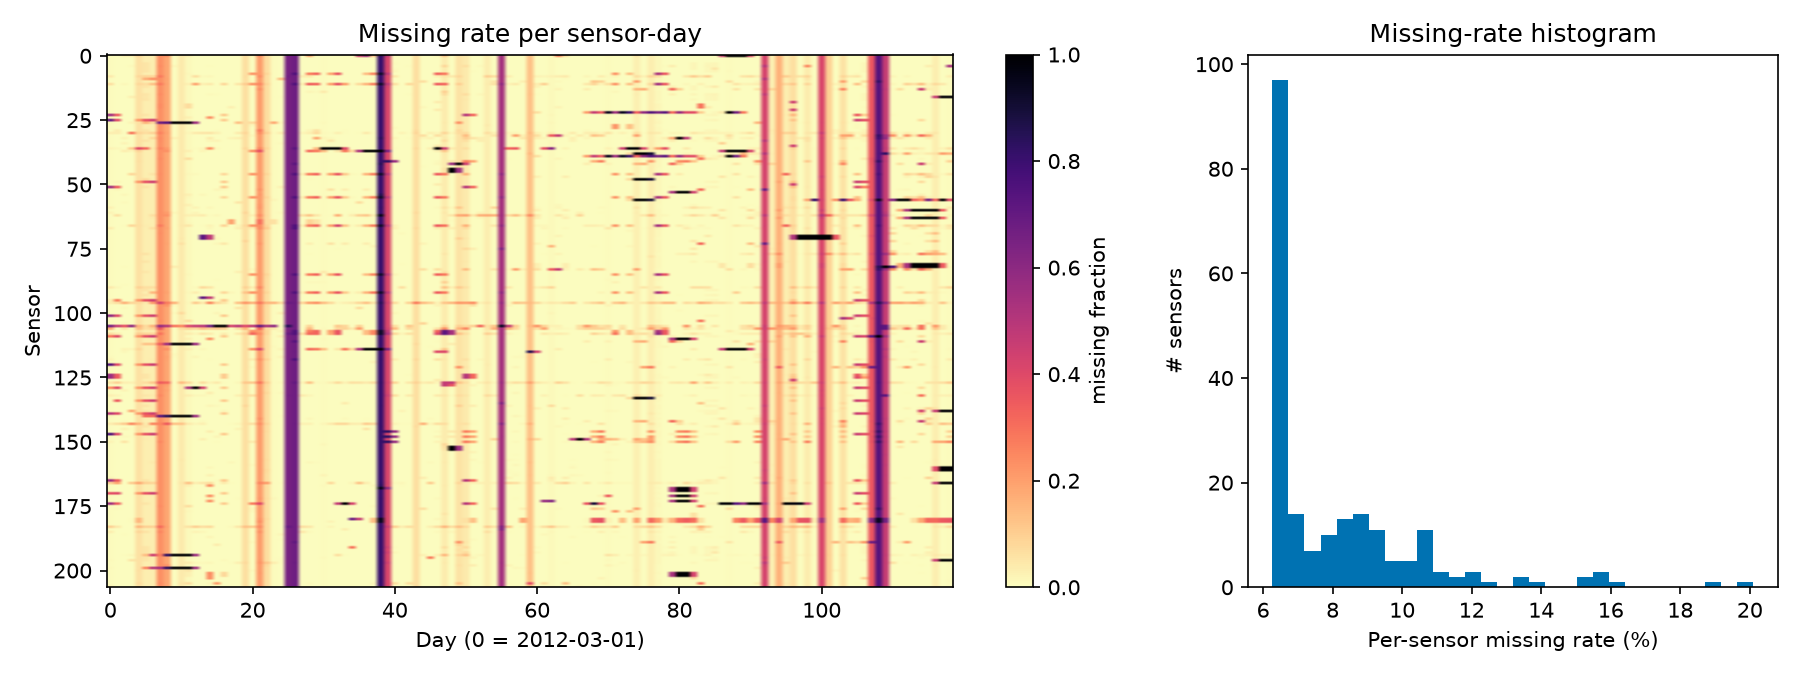
\includegraphics[width=1.00\linewidth]{../../results/figures/eda/01_missingness.png}\\[2pt]{\footnotesize\itshape Figure 1. Missing rate per sensor-day (left) and per-sensor missing-rate histogram (right).}\end{figure}

\subsection*{6.2 Daily profile and weekly pattern}\addcontentsline{toc}{subsection}{6.2 Daily profile and weekly pattern}
Weekday mean speed bottoms out at 45.3 mph around 17:30; weekends only drop to 56.8 mph (around 13:30). Across the week, slot means range from 42.5 to 65.7 mph, with congestion confined to weekday rush hours.

\begin{figure}[H]\centering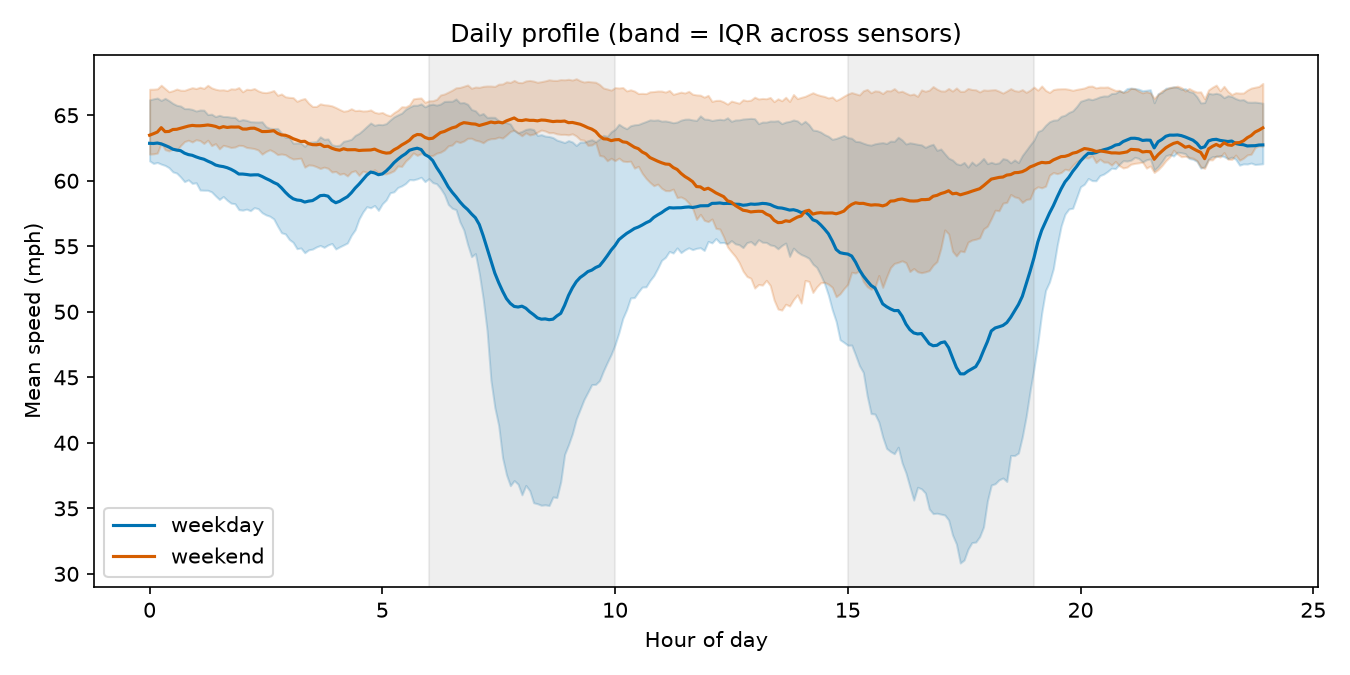
\includegraphics[width=0.89\linewidth]{../../results/figures/eda/02_daily_profile.png}\\[2pt]{\footnotesize\itshape Figure 2. Mean speed by time of day, weekday vs weekend (band: interquartile range across sensors; shaded: peak windows).}\end{figure}

\begin{figure}[H]\centering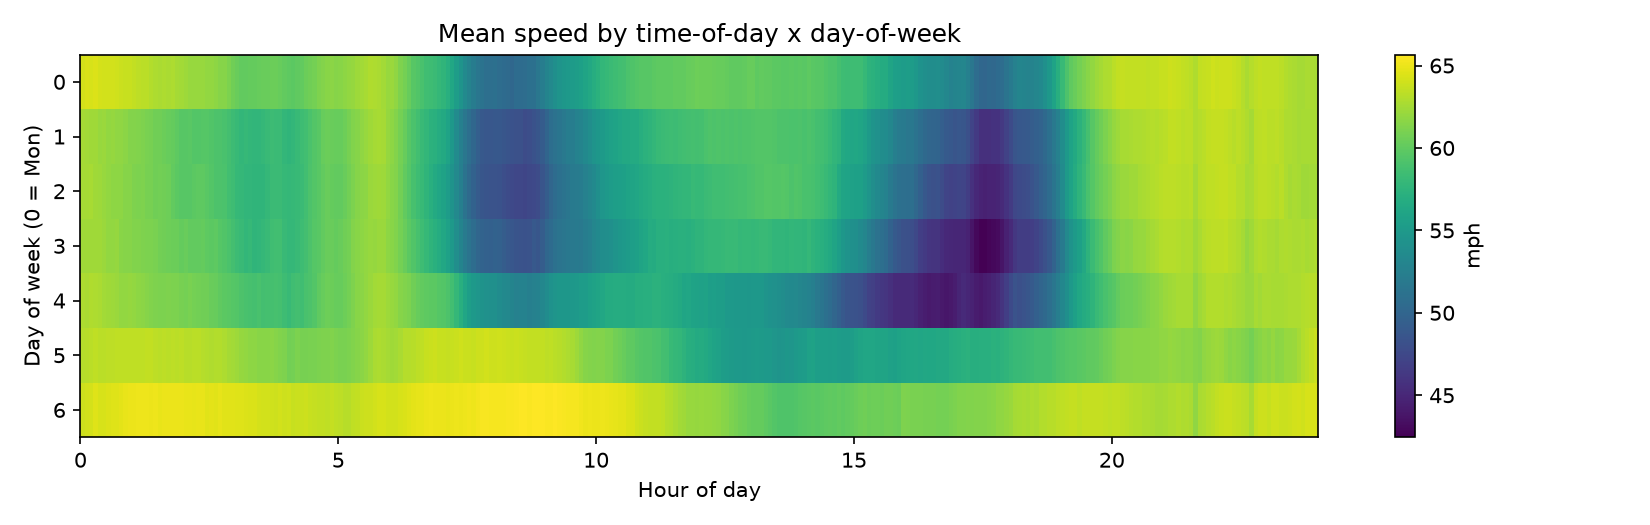
\includegraphics[width=1.00\linewidth]{../../results/figures/eda/03_tod_dow_heatmap.png}\\[2pt]{\footnotesize\itshape Figure 3. Mean speed by time of day \ensuremath{\times} day of week.}\end{figure}

\subsection*{6.3 Speed distribution}\addcontentsline{toc}{subsection}{6.3 Speed distribution}
Overall mean 58.46 mph. 10.9\% of observations are below 40 mph overall, 26.9\% during weekday peaks and 5.8\% off-peak (mean 51.5 mph at peak vs 60.6 mph off-peak). Congestion is the minority class and dominates errors.

\begin{figure}[H]\centering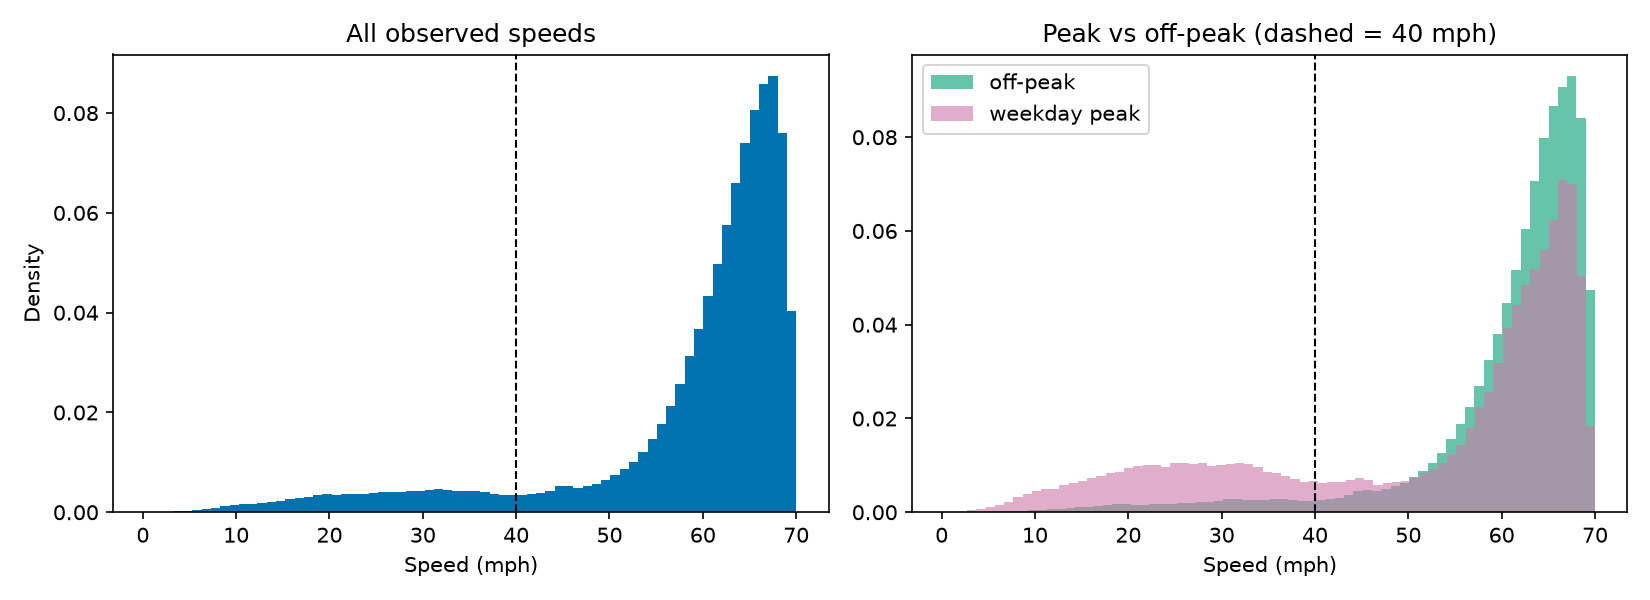
\includegraphics[width=1.00\linewidth]{../../results/figures/eda/04_speed_distribution.png}\\[2pt]{\footnotesize\itshape Figure 4. Speed distribution overall and peak vs off-peak (dashed: 40 mph).}\end{figure}

\subsection*{6.4 Autocorrelation}\addcontentsline{toc}{subsection}{6.4 Autocorrelation}
Three representative sensors (lowest, median and highest variance among sensors with < 10\% missing) show autocorrelation at the daily lag of 288 steps of 0.034, 0.400, 0.455 respectively: daily seasonality exists but its strength varies by sensor. Short-lag autocorrelation is very strong, which justifies a 12-step history and makes nearby windows dependent (a reason for chronological splits and autocorrelation-robust significance tests).

\begin{figure}[H]\centering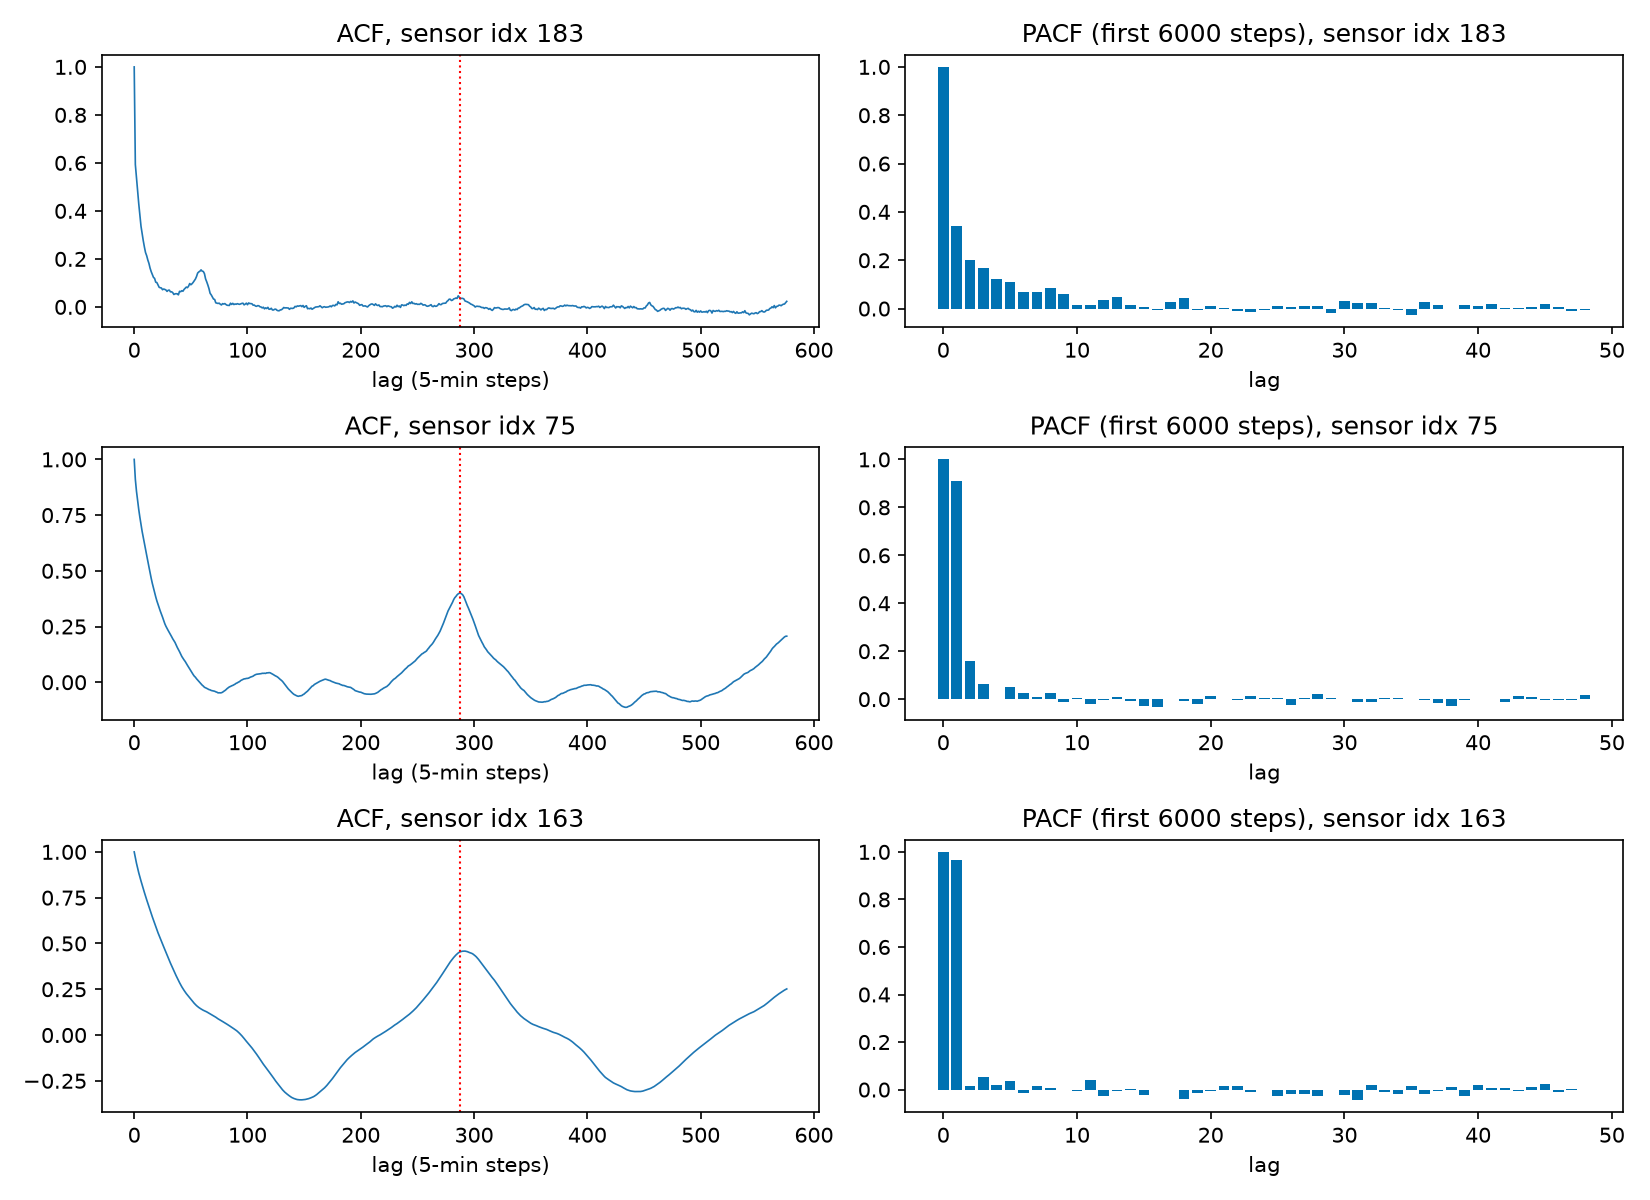
\includegraphics[width=0.92\linewidth]{../../results/figures/eda/05_acf_pacf.png}\\[2pt]{\footnotesize\itshape Figure 5. ACF (left, red line at lag 288) and PACF (right) for three sensors.}\end{figure}

\subsection*{6.5 Spatial dependence}\addcontentsline{toc}{subsection}{6.5 Spatial dependence}
{\scriptsize\renewcommand{\arraystretch}{1.15}\begin{longtable}{>{\raggedright\arraybackslash}p{0.1000\dimexpr\linewidth-20\tabcolsep\relax}>{\raggedright\arraybackslash}p{0.1000\dimexpr\linewidth-20\tabcolsep\relax}>{\raggedright\arraybackslash}p{0.1000\dimexpr\linewidth-20\tabcolsep\relax}>{\raggedright\arraybackslash}p{0.1000\dimexpr\linewidth-20\tabcolsep\relax}>{\raggedright\arraybackslash}p{0.1000\dimexpr\linewidth-20\tabcolsep\relax}>{\raggedright\arraybackslash}p{0.1000\dimexpr\linewidth-20\tabcolsep\relax}>{\raggedright\arraybackslash}p{0.1000\dimexpr\linewidth-20\tabcolsep\relax}>{\raggedright\arraybackslash}p{0.1000\dimexpr\linewidth-20\tabcolsep\relax}>{\raggedright\arraybackslash}p{0.1000\dimexpr\linewidth-20\tabcolsep\relax}>{\raggedright\arraybackslash}p{0.1000\dimexpr\linewidth-20\tabcolsep\relax}}
\toprule
\textbf{Hops} & \textbf{1} & \textbf{2} & \textbf{3} & \textbf{4} & \textbf{5} & \textbf{6} & \textbf{7} & \textbf{8} & \textbf{unreachable} \\
\midrule
\endhead
\bottomrule
\endlastfoot
Median correlation & 0.446 & 0.245 & 0.194 & 0.179 & 0.164 & 0.150 & 0.140 & 0.144 & 0.196 \\
\end{longtable}}
{\footnotesize\itshape Table 9. Median pairwise speed correlation by shortest-path distance in the (undirected) graph, training period.}\par\medskip

\begin{figure}[H]\centering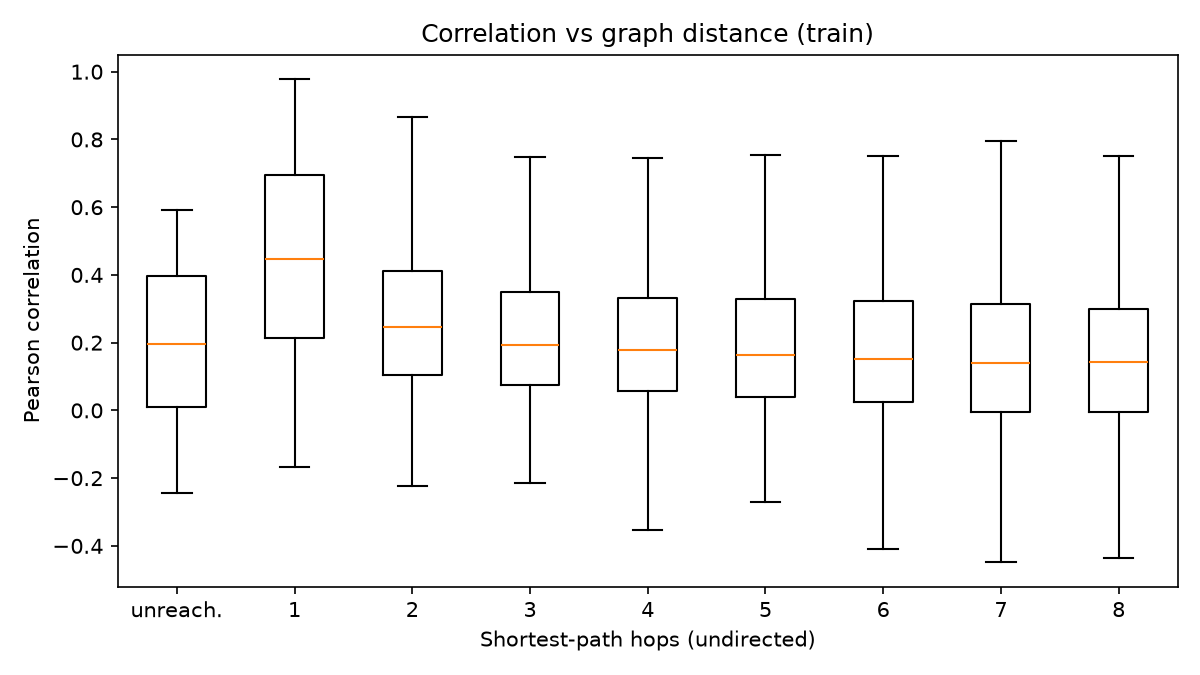
\includegraphics[width=0.89\linewidth]{../../results/figures/eda/06_corr_vs_hops.png}\\[2pt]{\footnotesize\itshape Figure 6. Correlation vs graph distance. Neighbours are clearly more informative than distant sensors.}\end{figure}

\subsection*{6.6 Propagation evidence (lagged cross-correlation)}\addcontentsline{toc}{subsection}{6.6 Propagation evidence (lagged cross-correlation)}
For every directed edge (i \ensuremath{\rightarrow} j, j downstream) with both sensors < 10\% missing, speeds are detrended by the training time-of-day mean and the correlation corr(z\_\allowbreak{}down(t), z\_\allowbreak{}up(t + lag)) is computed for lags \ensuremath{-}12\ldots{}+12. A positive peak lag means the upstream sensor changes after the downstream one, i.e. congestion moving upstream.

{\footnotesize\renewcommand{\arraystretch}{1.15}\begin{longtable}{>{\raggedright\arraybackslash}p{0.2800\dimexpr\linewidth-10\tabcolsep\relax}>{\raggedright\arraybackslash}p{0.1400\dimexpr\linewidth-10\tabcolsep\relax}>{\raggedright\arraybackslash}p{0.1900\dimexpr\linewidth-10\tabcolsep\relax}>{\raggedright\arraybackslash}p{0.1900\dimexpr\linewidth-10\tabcolsep\relax}>{\raggedright\arraybackslash}p{0.2000\dimexpr\linewidth-10\tabcolsep\relax}}
\toprule
\textbf{Period} & \textbf{Pairs} & \textbf{Peak lag > 0} & \textbf{Peak lag = 0} & \textbf{Peak lag < 0} \\
\midrule
\endhead
\bottomrule
\endlastfoot
All times & 1,228 & 38\% & 32\% & 30\% \\
Weekday peak hours & 1,228 & 50\% & 12\% & 38\% \\
\end{longtable}}
{\footnotesize\itshape Table 10. Distribution of the peak lag over all adjacent pairs.}\par\medskip

Reading: spatial dependence is clear; directional propagation is only modestly supported. The strongest pairs peak at lag 0 (adjacent sensors move together at 5-minute resolution); at peak hours positive lags outnumber negative ones, but many pairs show the opposite sign. Example pairs in Figure 9 are chosen by stated rules (top correlation; largest non-zero lag with correlation \ensuremath{\geq} 0.5), never by eye.

\begin{figure}[H]\centering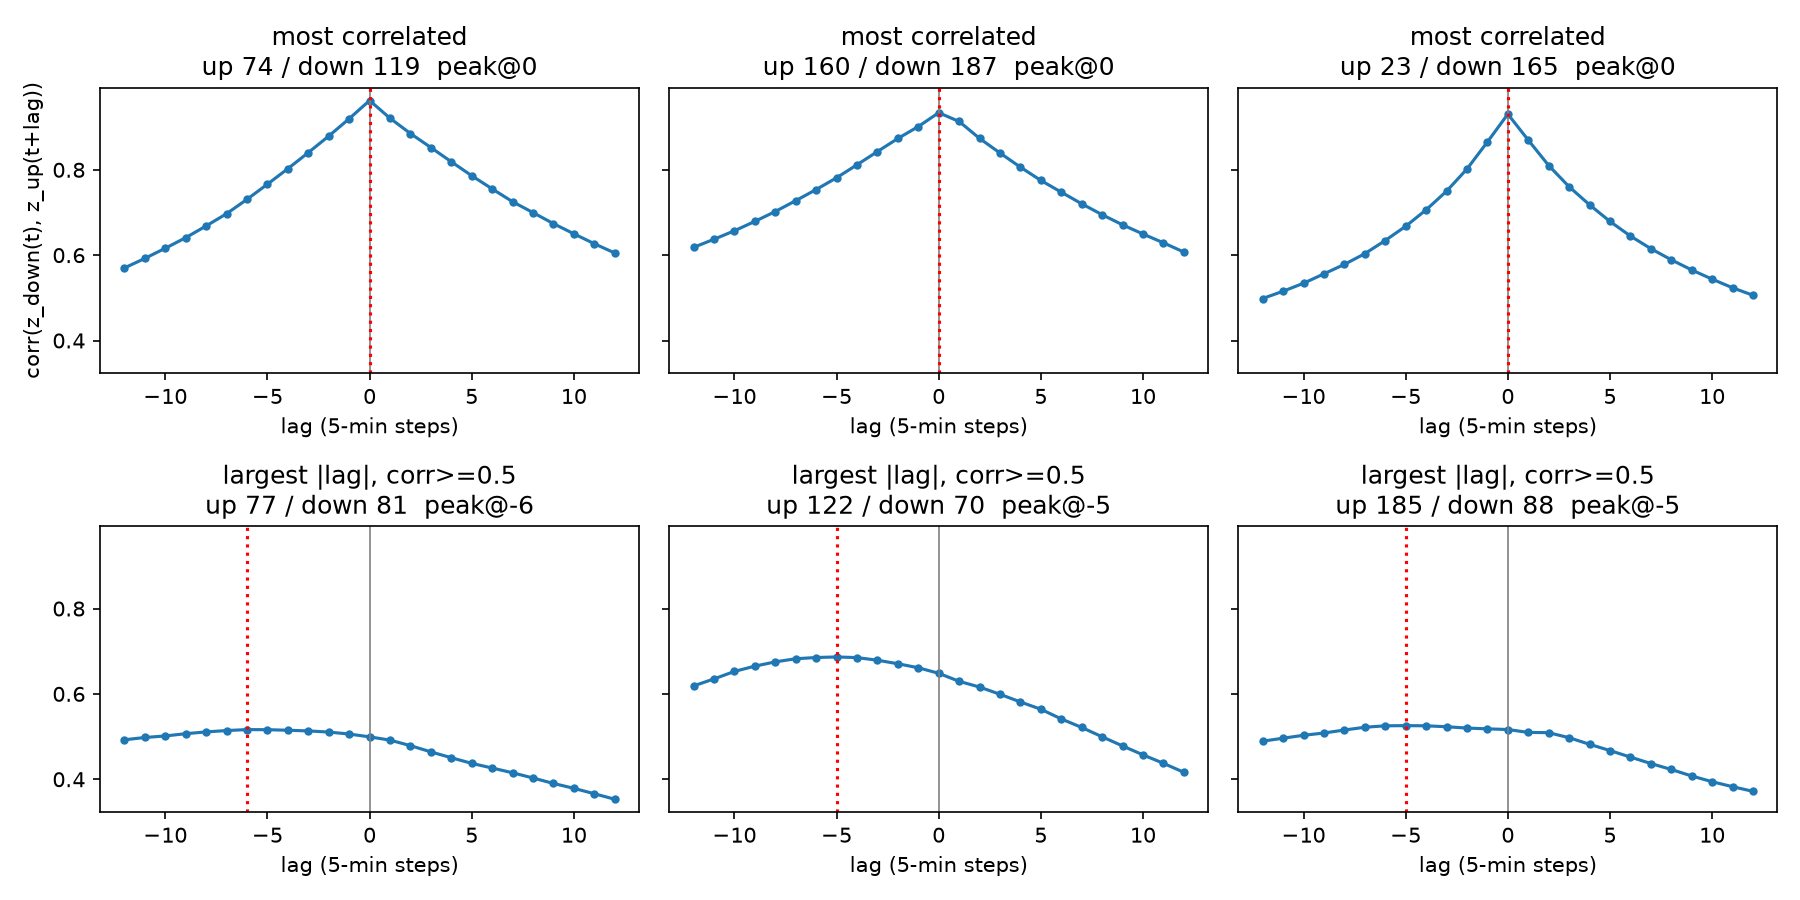
\includegraphics[width=1.00\linewidth]{../../results/figures/eda/07_lagged_xcorr.png}\\[2pt]{\footnotesize\itshape Figure 7. Cross-correlation curves for six pairs chosen by rule.}\end{figure}

\begin{figure}[H]\centering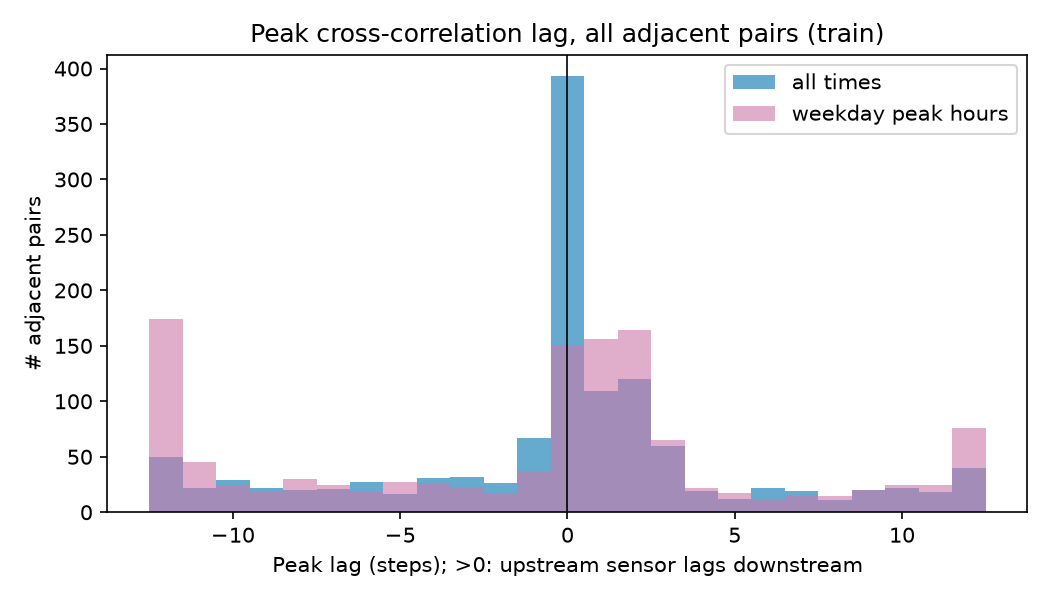
\includegraphics[width=0.79\linewidth]{../../results/figures/eda/07b_peak_lag_hist.png}\\[2pt]{\footnotesize\itshape Figure 8. Peak lag across all adjacent pairs: all times vs weekday peak hours.}\end{figure}

\subsection*{6.7 Where congestion happens}\addcontentsline{toc}{subsection}{6.7 Where congestion happens}
The median sensor is below 40 mph for 27\% of weekday-peak time; 119 sensors exceed 20\% and the worst is congested 100\% of the time. 47 sensors have a mean speed below 55 mph. Interactive maps: \texttt{results/\allowbreak{}maps/\allowbreak{}eda\_\allowbreak{}sensors.html}, \texttt{results/\allowbreak{}maps/\allowbreak{}eda\_\allowbreak{}congestion\_\allowbreak{}frequency.html}.

\begin{figure}[H]\centering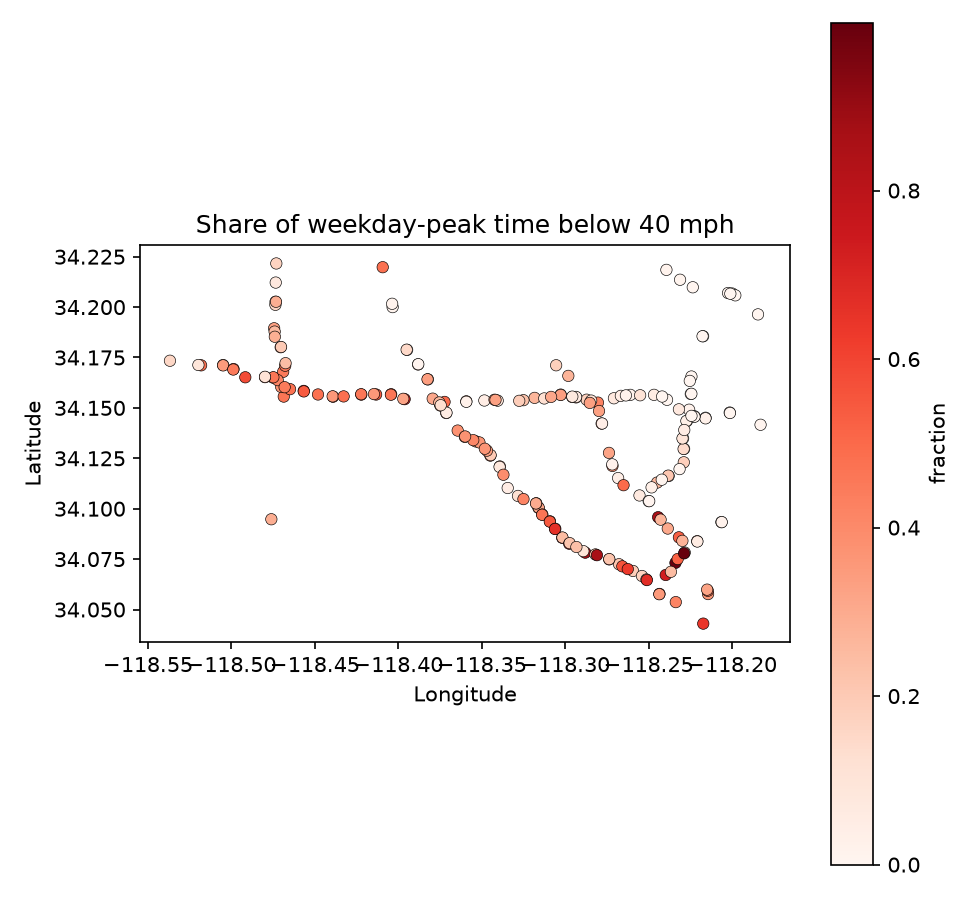
\includegraphics[width=0.73\linewidth]{../../results/figures/eda/09_congestion_frequency_map.png}\\[2pt]{\footnotesize\itshape Figure 9. Share of weekday-peak time below 40 mph per sensor.}\end{figure}

\subsection*{6.8 Split comparability}\addcontentsline{toc}{subsection}{6.8 Split comparability}
{\footnotesize\renewcommand{\arraystretch}{1.15}\begin{longtable}{>{\raggedright\arraybackslash}p{0.1600\dimexpr\linewidth-10\tabcolsep\relax}>{\raggedright\arraybackslash}p{0.2100\dimexpr\linewidth-10\tabcolsep\relax}>{\raggedright\arraybackslash}p{0.2100\dimexpr\linewidth-10\tabcolsep\relax}>{\raggedright\arraybackslash}p{0.2100\dimexpr\linewidth-10\tabcolsep\relax}>{\raggedright\arraybackslash}p{0.2100\dimexpr\linewidth-10\tabcolsep\relax}}
\toprule
\textbf{Split} & \textbf{Weekday share} & \textbf{Peak share} & \textbf{Missing rate} & \textbf{Mean speed (mph)} \\
\midrule
\endhead
\bottomrule
\endlastfoot
train & 71.2\% & 23.7\% & 7.1\% & 58.58 \\
val & 66.4\% & 22.0\% & 7.0\% & 58.90 \\
test & 74.8\% & 25.2\% & 12.1\% & 57.77 \\
\end{longtable}}
{\footnotesize\itshape Table 11. Composition of the three periods.}\par\medskip

\begin{figure}[H]\centering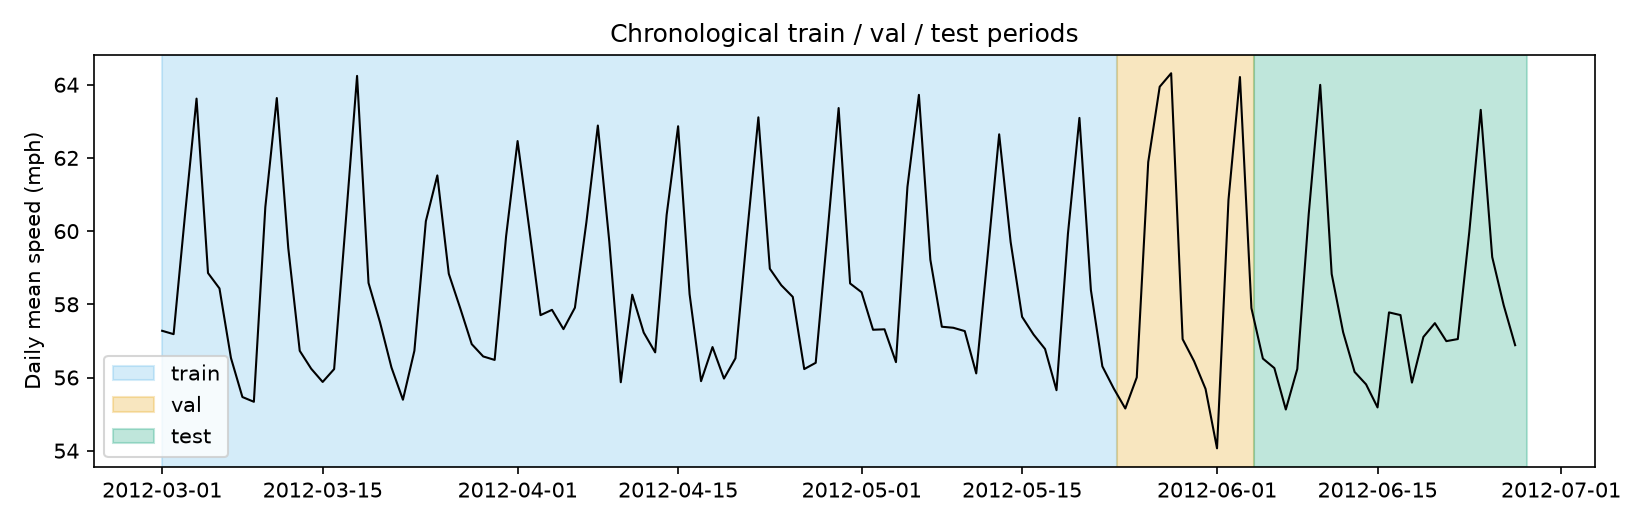
\includegraphics[width=1.00\linewidth]{../../results/figures/eda/10_split_timeline.png}\\[2pt]{\footnotesize\itshape Figure 10. Daily mean speed with the train /\allowbreak{} validation /\allowbreak{} test periods.}\end{figure}

\clearpage
\section*{7. Evaluation protocol (identical for all models)}\addcontentsline{toc}{section}{7. Evaluation protocol (identical for all models)}
\subsection*{7.1 Common prediction format}\addcontentsline{toc}{subsection}{7.1 Common prediction format}
Every model writes \texttt{results/\allowbreak{}predictions/\allowbreak{}<model>[\_\allowbreak{}seed<k>].npz} with \texttt{y\_\allowbreak{}pred} and \texttt{y\_\allowbreak{}true} [S, F, N] in mph, \texttt{mask} [S, F, N], \texttt{target\_\allowbreak{}ts} [S, F], \texttt{sensor\_\allowbreak{}ids} and metadata. The evaluator first asserts that every file has exactly the same test timestamps, masks and sensors as persistence (S = 6,832 test windows \ensuremath{\times} 12 horizons \ensuremath{\times} 207 sensors). Horizons a model does not produce (per-segment XGBoost trains only 15/\allowbreak{}30/\allowbreak{}60 minutes) are stored as NaN and skipped.

\subsection*{7.2 Metrics (masked, in mph)}\addcontentsline{toc}{subsection}{7.2 Metrics (masked, in mph)}
\begin{eqbox}MAE = \ensuremath{\Sigma} m\ensuremath{\cdot}|y \ensuremath{-} \ensuremath{\hat{y}}| /\allowbreak{} \ensuremath{\Sigma} m        RMSE = \ensuremath{\sqrt{\ }}( \ensuremath{\Sigma} m\ensuremath{\cdot}(y \ensuremath{-} \ensuremath{\hat{y}})\ensuremath{^{2}} /\allowbreak{} \ensuremath{\Sigma} m )        MAPE = 100 \ensuremath{\cdot} \ensuremath{\Sigma} m\ensuremath{'}\ensuremath{\cdot}|y \ensuremath{-} \ensuremath{\hat{y}}|/\allowbreak{}y /\allowbreak{} \ensuremath{\Sigma} m\ensuremath{'},   m\ensuremath{'} = m \ensuremath{\wedge} (y \ensuremath{\geq} 1 mph)\end{eqbox}

An all-masked slice returns NaN, never 0. NaN predictions are removed from the mask. Hand-computed unit tests cover these cases (ADR-005).

\subsection*{7.3 Slices}\addcontentsline{toc}{subsection}{7.3 Slices}
\begin{itemize}[nosep,leftmargin=*]
\item Every horizon 1\ldots{}12; headline tables at 3, 6, 12 steps (15, 30, 60 minutes).
\item Peak AM (06:00--10:00), peak PM (15:00--19:00), peak (either), off-peak weekday, weekend --- judged on the target timestamp.
\item Congested (true speed < 40 mph) vs free-flow (\ensuremath{\geq} 40 mph).
\item Per sensor (for maps).
\end{itemize}

\subsection*{7.4 Statistical significance}\addcontentsline{toc}{subsection}{7.4 Statistical significance}
\begin{itemize}[nosep,leftmargin=*]
\item \textbf{Diebold--Mariano (DM) test} on the per-timestamp loss differential d\_\allowbreak{}t = mean over sensors |e\ensuremath{_{1}}| \ensuremath{-} mean |e\ensuremath{_{2}}| (sensors observed in both), per headline horizon. Long-run variance: Newey--West with a Bartlett kernel and L = max(h \ensuremath{-} 1, \ensuremath{\lceil}T\^{}(1/\allowbreak{}3)\ensuremath{\rceil}) lags; Harvey--Leybourne--Newbold small-sample correction; Student t with T \ensuremath{-} 1 degrees of freedom. Negative statistic: the first model has lower loss.
\item For multi-seed models the test is run per seed pair; we report the median statistic and the \textbf{largest} (most conservative) p-value.
\item \textbf{Day-block bootstrap:} whole days of target timestamps are resampled with replacement (1,000 draws, seed 42) for 95\% intervals; paired versions resample the same days for both models so day difficulty cancels.
\end{itemize}

\subsection*{7.5 Automatic sanity checks}\addcontentsline{toc}{subsection}{7.5 Automatic sanity checks}
\begin{itemize}[nosep,leftmargin=*]
\item Any model with MAE at 60 minutes below 3.0 mph triggers a leakage warning (published strong graph models report \ensuremath{\approx} 3.5).
\item Any learned model not beating persistence at 15 minutes triggers ``something is broken''.
\item Final run: ``no warnings''.
\end{itemize}

\clearpage
\section*{8. Baselines}\addcontentsline{toc}{section}{8. Baselines}
\begin{itemize}[nosep,leftmargin=*]
\item \textbf{Persistence:} \ensuremath{\hat{y}}(t + h) = last observed value in the input window (past-only forward fill up to 11 steps; time-of-day mean if the whole window is missing).
\item \textbf{Historical average:} mean of that sensor at the same (day-of-week, 5-minute slot), training period only (7 \ensuremath{\times} 288 \ensuremath{\times} 207 table); falls back to the slot mean.
\item \textbf{Seasonal naive:} \ensuremath{\hat{y}}(t + h) = y(t + h \ensuremath{-} 288) (same time yesterday); when that value is missing it falls back to the historical average (12.61\% of entries).
\end{itemize}

{\scriptsize\renewcommand{\arraystretch}{1.15}\begin{longtable}{>{\raggedright\arraybackslash}p{0.1000\dimexpr\linewidth-20\tabcolsep\relax}>{\raggedright\arraybackslash}p{0.1000\dimexpr\linewidth-20\tabcolsep\relax}>{\raggedright\arraybackslash}p{0.1000\dimexpr\linewidth-20\tabcolsep\relax}>{\raggedright\arraybackslash}p{0.1000\dimexpr\linewidth-20\tabcolsep\relax}>{\raggedright\arraybackslash}p{0.1000\dimexpr\linewidth-20\tabcolsep\relax}>{\raggedright\arraybackslash}p{0.1000\dimexpr\linewidth-20\tabcolsep\relax}>{\raggedright\arraybackslash}p{0.1000\dimexpr\linewidth-20\tabcolsep\relax}>{\raggedright\arraybackslash}p{0.1000\dimexpr\linewidth-20\tabcolsep\relax}>{\raggedright\arraybackslash}p{0.1000\dimexpr\linewidth-20\tabcolsep\relax}>{\raggedright\arraybackslash}p{0.1000\dimexpr\linewidth-20\tabcolsep\relax}}
\toprule
\textbf{Baseline} & \textbf{MAE 15} & \textbf{MAE 30} & \textbf{MAE 60} & \textbf{RMSE 15} & \textbf{RMSE 30} & \textbf{RMSE 60} & \textbf{MAPE 15} & \textbf{MAPE 30} & \textbf{MAPE 60} \\
\midrule
\endhead
\bottomrule
\endlastfoot
Persistence & 3.49 & 4.20 & 5.37 & 6.39 & 8.02 & 10.30 & 8.60 & 10.83 & 14.48 \\
Historical average & 4.19 & 4.19 & 4.19 & 7.86 & 7.86 & 7.86 & 13.06 & 13.06 & 13.06 \\
Seasonal naive & 5.50 & 5.50 & 5.50 & 10.71 & 10.71 & 10.71 & 15.57 & 15.57 & 15.57 \\
\end{longtable}}
{\footnotesize\itshape Table 12. Baseline test errors (mph; MAPE in \%).}\par\medskip

The historical average is flat across horizons because it ignores the current state; its 4.19 mph is close to the 4.16 reported for the historical average in the DCRNN paper, a useful external check of the pipeline.

\clearpage
\section*{9. Phase 1 --- machine learning}\addcontentsline{toc}{section}{9. Phase 1 --- machine learning}
\subsection*{9.1 Tabular features}\addcontentsline{toc}{subsection}{9.1 Tabular features}
One row per (sensor, anchor time); all features use data at or before the anchor (tested by perturbing the future).

{\scriptsize\renewcommand{\arraystretch}{1.15}\begin{longtable}{>{\raggedright\arraybackslash}p{0.2400\dimexpr\linewidth-6\tabcolsep\relax}>{\raggedright\arraybackslash}p{0.6200\dimexpr\linewidth-6\tabcolsep\relax}>{\raggedright\arraybackslash}p{0.1400\dimexpr\linewidth-6\tabcolsep\relax}}
\toprule
\textbf{Group} & \textbf{Features} & \textbf{Count} \\
\midrule
\endhead
\bottomrule
\endlastfoot
Lags & lag\_\allowbreak{}0 \ldots{} lag\_\allowbreak{}11 (imputed speed) & 12 \\
Rolling statistics & mean, std, min, max over 3, 6, 12 steps & 12 \\
Differences & lag\_\allowbreak{}0 \ensuremath{-} lag\_\allowbreak{}1, lag\_\allowbreak{}0 \ensuremath{-} lag\_\allowbreak{}3 & 2 \\
Missing flags & miss\_\allowbreak{}0 \ldots{} miss\_\allowbreak{}11 and n\_\allowbreak{}missing\_\allowbreak{}window & 13 \\
Calendar (at anchor) & tod\_\allowbreak{}sin, tod\_\allowbreak{}cos, dow\_\allowbreak{}sin, dow\_\allowbreak{}cos, is\_\allowbreak{}weekend, is\_\allowbreak{}holiday & 6 \\
Static (pooled models) & sensor\_\allowbreak{}idx (categorical), latitude, longitude, in\_\allowbreak{}degree, out\_\allowbreak{}degree & 5 \\
Neighbour (XGB-spatial) & upstream and downstream weighted means at lags 0--2 (6), 2-hop mean, own \ensuremath{-} upstream, own \ensuremath{-} downstream & 9 \\
Daily lag (side experiment) & lag\_\allowbreak{}288 (same time yesterday) & 1 \\
\end{longtable}}
{\footnotesize\itshape Table 13. Feature groups. Per-segment models use 45 features, pooled models 50, XGB-spatial 59, the daily-lag run 51.}\par\medskip

Neighbour features use row-normalised \texttt{W} (downstream senders) and \texttt{W\ensuremath{^{\top}}} (upstream senders); sensors with no neighbour in a direction get NaN, which XGBoost handles natively.

\subsection*{9.2 Models}\addcontentsline{toc}{subsection}{9.2 Models}
\begin{itemize}[nosep,leftmargin=*]
\item \textbf{XGBoost per-segment:} one model per sensor per headline horizon, 207 \ensuremath{\times} 3 = 621 models, \textasciitilde{}24k rows each, \texttt{tree\_\allowbreak{}method=hist}, single-threaded per model and parallel over sensors.
\item \textbf{XGBoost global (pooled):} one model per horizon (12 models) across all sensors with sensor id as a categorical feature.
\item \textbf{Random Forest (multi-output):} one pooled forest that predicts all 12 horizons jointly (joint squared-error split criterion); rows with any missing horizon are dropped.
\item \textbf{XGBoost spatial:} the pooled model plus the 9 neighbour features --- the bridge experiment that tests how much of the graph benefit hand-made features capture.
\end{itemize}

\subsection*{9.3 Hyperparameter tuning (Optuna, validation only)}\addcontentsline{toc}{subsection}{9.3 Hyperparameter tuning (Optuna, validation only)}
TPE sampler (seed 42). XGBoost objective: validation MAE at horizon 6 on 300,000 sampled training rows and 150,000 validation rows, early stopping 30 rounds, tree cap 400; per-segment tuning pools 20 random sensors with shared hyperparameters. Random Forest: mean validation MAE over all 12 horizons on 60,000 /\allowbreak{} 30,000 rows. The test split is never touched during tuning.

{\footnotesize\renewcommand{\arraystretch}{1.15}\begin{longtable}{>{\raggedright\arraybackslash}p{0.4000\dimexpr\linewidth-8\tabcolsep\relax}>{\raggedright\arraybackslash}p{0.1500\dimexpr\linewidth-8\tabcolsep\relax}>{\raggedright\arraybackslash}p{0.2200\dimexpr\linewidth-8\tabcolsep\relax}>{\raggedright\arraybackslash}p{0.2300\dimexpr\linewidth-8\tabcolsep\relax}}
\toprule
\textbf{Model} & \textbf{Trials} & \textbf{Best val MAE} & \textbf{Median val MAE} \\
\midrule
\endhead
\bottomrule
\endlastfoot
XGBoost global (pooled) & 15 & 3.1530 & 3.2035 \\
XGBoost spatial & 15 & 3.0874 & 3.1451 \\
XGBoost per-segment & 15 & 3.5945 & 3.6220 \\
Random Forest (multi-output) & 6 & 3.5295 & 3.5643 \\
\end{longtable}}
{\footnotesize\itshape Table 14. Tuning summary (validation MAE in mph; tuning subsets differ between models, so values are not mutually comparable).}\par\medskip

{\scriptsize\renewcommand{\arraystretch}{1.15}\begin{longtable}{>{\raggedright\arraybackslash}p{0.2000\dimexpr\linewidth-10\tabcolsep\relax}>{\raggedright\arraybackslash}p{0.3000\dimexpr\linewidth-10\tabcolsep\relax}>{\raggedright\arraybackslash}p{0.1700\dimexpr\linewidth-10\tabcolsep\relax}>{\raggedright\arraybackslash}p{0.1700\dimexpr\linewidth-10\tabcolsep\relax}>{\raggedright\arraybackslash}p{0.1600\dimexpr\linewidth-10\tabcolsep\relax}}
\toprule
\textbf{Parameter} & \textbf{Search range} & \textbf{Per-segment} & \textbf{Global} & \textbf{Spatial} \\
\midrule
\endhead
\bottomrule
\endlastfoot
max\_\allowbreak{}depth & 3 -- 10 & 9 & 10 & 10 \\
learning\_\allowbreak{}rate & 0.02 -- 0.3 (log) & 0.0343 & 0.0402 & 0.0402 \\
subsample & 0.5 -- 1.0 & 0.5028 & 0.5435 & 0.5435 \\
colsample\_\allowbreak{}bytree & 0.5 -- 1.0 & 0.9077 & 0.9238 & 0.9238 \\
min\_\allowbreak{}child\_\allowbreak{}weight & 1 -- 20 & 15 & 6 & 6 \\
reg\_\allowbreak{}lambda & 0.001 -- 10 (log) & 0.8242 & 5.2222 & 5.2222 \\
gamma & 0 -- 5 & 3.8564 & 3.7865 & 3.7865 \\
objective & squared error | absolute error | pseudo-Huber & reg:absoluteerror & reg:absoluteerror & reg:absoluteerror \\
\end{longtable}}
{\footnotesize\itshape Table 15. XGBoost search space and the selected values (absolute-error loss chosen for all three). Global and spatial chose identical values: same seed and the same best trial index.}\par\medskip

Random Forest search: n\_\allowbreak{}estimators 60--150, max\_\allowbreak{}depth 8--30, max\_\allowbreak{}features \ensuremath{\in} \{0.2, 0.33, 0.5\}, min\_\allowbreak{}samples\_\allowbreak{}leaf 1--20, max\_\allowbreak{}samples 0.5. Selected: 135 trees, max\_\allowbreak{}depth 12, max\_\allowbreak{}features 0.5, min\_\allowbreak{}samples\_\allowbreak{}leaf 11, max\_\allowbreak{}samples 0.5.

\subsection*{9.4 Training budget (reduced for a laptop, ADR-006)}\addcontentsline{toc}{subsection}{9.4 Training budget (reduced for a laptop, ADR-006)}
{\scriptsize\renewcommand{\arraystretch}{1.15}\begin{longtable}{>{\raggedright\arraybackslash}p{0.2200\dimexpr\linewidth-8\tabcolsep\relax}>{\raggedright\arraybackslash}p{0.3300\dimexpr\linewidth-8\tabcolsep\relax}>{\raggedright\arraybackslash}p{0.1500\dimexpr\linewidth-8\tabcolsep\relax}>{\raggedright\arraybackslash}p{0.3000\dimexpr\linewidth-8\tabcolsep\relax}}
\toprule
\textbf{Model} & \textbf{Training rows} & \textbf{Training time} & \textbf{Notes} \\
\midrule
\endhead
\bottomrule
\endlastfoot
XGBoost global & \ensuremath{\approx} 1.15 million per horizon (25\% sample) & 755 s & 12 horizons; every model used 398--399 of 400 trees \\
XGBoost spatial & \ensuremath{\approx} 1.15 million per horizon (25\% sample) & 1252 s & 12 horizons; every model used 398--399 of 400 trees \\
XGBoost per-segment & all rows of each sensor & 198 s & 621 models \\
Random Forest & 444,904 of 4,449,042 complete rows (10\%) & 56 s & 10.3\% of rows dropped (a horizon missing) \\
XGBoost global + daily lag & \ensuremath{\approx} 1.15 million per horizon & 1173 s & side experiment \\
\end{longtable}}
{\footnotesize\itshape Table 16. Training data and wall-clock time (6 CPU workers, low priority, Apple M3 Pro).}\par\medskip

\begin{callout}Early stopping never triggered for the pooled XGBoost models: the best iteration was 398--399 of the 400-tree cap at every horizon. More trees (and more training rows) would very likely lower their error further. The reported ML numbers are therefore conservative.\end{callout}

\subsection*{9.5 Phase 1 results}\addcontentsline{toc}{subsection}{9.5 Phase 1 results}
{\scriptsize\renewcommand{\arraystretch}{1.15}\begin{longtable}{>{\raggedright\arraybackslash}p{0.1000\dimexpr\linewidth-20\tabcolsep\relax}>{\raggedright\arraybackslash}p{0.1000\dimexpr\linewidth-20\tabcolsep\relax}>{\raggedright\arraybackslash}p{0.1000\dimexpr\linewidth-20\tabcolsep\relax}>{\raggedright\arraybackslash}p{0.1000\dimexpr\linewidth-20\tabcolsep\relax}>{\raggedright\arraybackslash}p{0.1000\dimexpr\linewidth-20\tabcolsep\relax}>{\raggedright\arraybackslash}p{0.1000\dimexpr\linewidth-20\tabcolsep\relax}>{\raggedright\arraybackslash}p{0.1000\dimexpr\linewidth-20\tabcolsep\relax}>{\raggedright\arraybackslash}p{0.1000\dimexpr\linewidth-20\tabcolsep\relax}>{\raggedright\arraybackslash}p{0.1000\dimexpr\linewidth-20\tabcolsep\relax}>{\raggedright\arraybackslash}p{0.1000\dimexpr\linewidth-20\tabcolsep\relax}}
\toprule
\textbf{Model} & \textbf{MAE 15} & \textbf{MAE 30} & \textbf{MAE 60} & \textbf{RMSE 15} & \textbf{RMSE 30} & \textbf{RMSE 60} & \textbf{MAPE 15} & \textbf{MAPE 30} & \textbf{MAPE 60} \\
\midrule
\endhead
\bottomrule
\endlastfoot
Persistence & 3.49 & 4.20 & 5.37 & 6.39 & 8.02 & 10.30 & 8.60 & 10.83 & 14.48 \\
Historical average & 4.19 & 4.19 & 4.19 & 7.86 & 7.86 & 7.86 & 13.06 & 13.06 & 13.06 \\
Seasonal naive & 5.50 & 5.50 & 5.50 & 10.71 & 10.71 & 10.71 & 15.57 & 15.57 & 15.57 \\
XGBoost per-segment & 2.86 & 3.28 & 3.68 & 5.60 & 6.62 & 7.52 & 7.92 & 9.77 & 11.65 \\
XGBoost global (pooled) & 2.88 & 3.33 & 3.78 & 5.69 & 6.80 & 7.76 & 7.87 & 9.90 & 12.11 \\
Random Forest (multi-output) & 3.14 & 3.80 & 4.73 & 5.70 & 6.89 & 8.25 & 8.50 & 10.87 & 14.27 \\
XGBoost spatial & 2.82 & 3.26 & 3.73 & 5.46 & 6.54 & 7.54 & 7.63 & 9.53 & 11.82 \\
\end{longtable}}
{\footnotesize\itshape Table 17. Phase 1 test errors (mph; MAPE in \%).}\par\medskip

\begin{itemize}[nosep,leftmargin=*]
\item XGB-spatial is best at 15 minutes (2.820) and 30 minutes (3.258); per-segment XGBoost is best at 60 minutes (3.684).
\item The forest is the weakest ML model (3.137 /\allowbreak{} 3.798 /\allowbreak{} 4.732); at 60 minutes it loses to the historical average.
\item All Phase 1 ML models beat persistence at every horizon; none comes close to the 3.0 mph leakage bound at 60 minutes.
\end{itemize}

\begin{figure}[H]\centering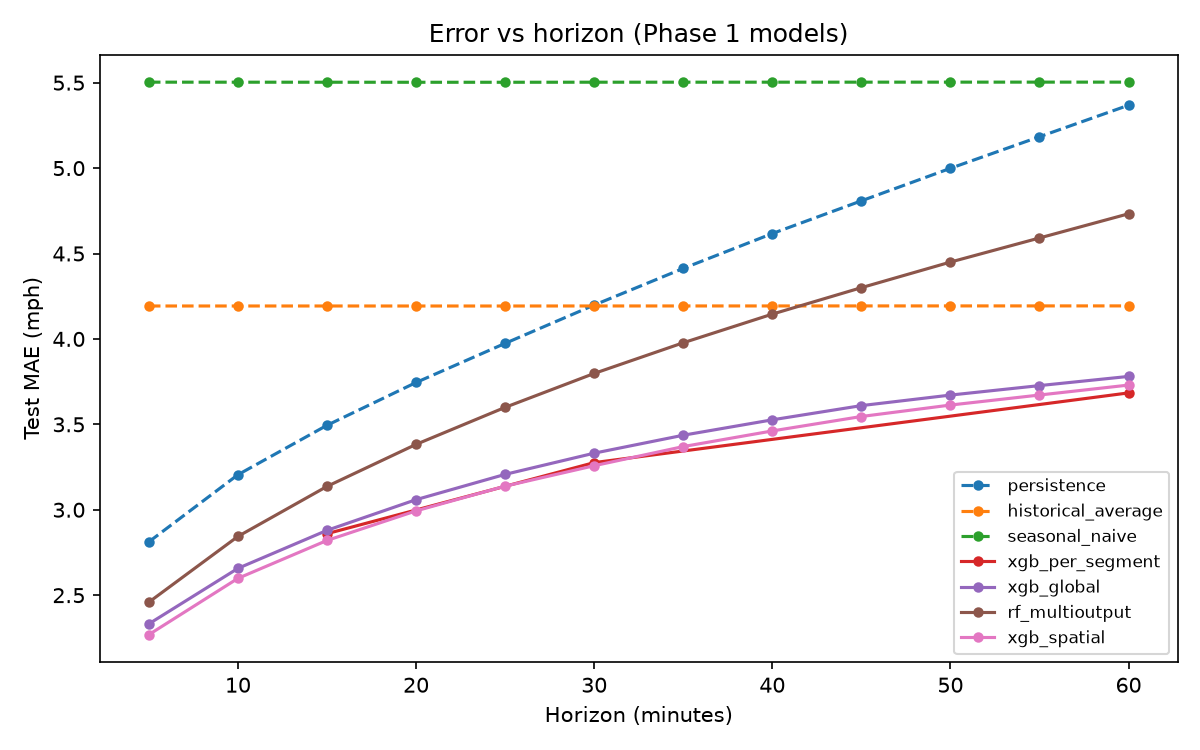
\includegraphics[width=0.89\linewidth]{../../results/figures/ml/error_vs_horizon.png}\\[2pt]{\footnotesize\itshape Figure 11. Test MAE vs horizon for baselines and Phase 1 models.}\end{figure}

\subsection*{9.6 What drives the trees (gain and TreeSHAP)}\addcontentsline{toc}{subsection}{9.6 What drives the trees (gain and TreeSHAP)}
TreeSHAP values come from XGBoost's exact \texttt{pred\_\allowbreak{}contribs} on 5,000 seeded test rows with observed targets.

{\scriptsize\renewcommand{\arraystretch}{1.15}\begin{longtable}{>{\raggedright\arraybackslash}p{0.2200\dimexpr\linewidth-6\tabcolsep\relax}>{\raggedright\arraybackslash}p{0.1200\dimexpr\linewidth-6\tabcolsep\relax}>{\raggedright\arraybackslash}p{0.6600\dimexpr\linewidth-6\tabcolsep\relax}}
\toprule
\textbf{Model} & \textbf{Horizon} & \textbf{Top 8 features by mean |SHAP| (mph)} \\
\midrule
\endhead
\bottomrule
\endlastfoot
XGBoost global (pooled) & 15 min & roll\_\allowbreak{}mean\_\allowbreak{}6 (3.79), lag\_\allowbreak{}0 (2.45), roll\_\allowbreak{}max\_\allowbreak{}3 (1.47), roll\_\allowbreak{}max\_\allowbreak{}6 (1.35), roll\_\allowbreak{}mean\_\allowbreak{}3 (0.89), sensor\_\allowbreak{}idx (0.72), tod\_\allowbreak{}cos (0.45), tod\_\allowbreak{}sin (0.24) \\
XGBoost global (pooled) & 60 min & roll\_\allowbreak{}mean\_\allowbreak{}6 (2.43), sensor\_\allowbreak{}idx (1.77), lag\_\allowbreak{}0 (1.45), tod\_\allowbreak{}cos (1.44), roll\_\allowbreak{}mean\_\allowbreak{}3 (1.19), roll\_\allowbreak{}max\_\allowbreak{}3 (1.18), tod\_\allowbreak{}sin (0.81), dow\_\allowbreak{}sin (0.46) \\
XGBoost spatial & 15 min & roll\_\allowbreak{}mean\_\allowbreak{}6 (3.32), lag\_\allowbreak{}0 (2.40), roll\_\allowbreak{}max\_\allowbreak{}3 (1.36), roll\_\allowbreak{}mean\_\allowbreak{}3 (1.16), roll\_\allowbreak{}max\_\allowbreak{}6 (1.16), sensor\_\allowbreak{}idx (0.82), up\_\allowbreak{}mean\_\allowbreak{}lag0 (0.46), down\_\allowbreak{}mean\_\allowbreak{}lag0 (0.44) \\
XGBoost spatial & 60 min & roll\_\allowbreak{}mean\_\allowbreak{}6 (2.32), sensor\_\allowbreak{}idx (1.79), lag\_\allowbreak{}0 (1.50), roll\_\allowbreak{}mean\_\allowbreak{}3 (1.28), tod\_\allowbreak{}cos (1.27), roll\_\allowbreak{}max\_\allowbreak{}3 (0.89), tod\_\allowbreak{}sin (0.77), up\_\allowbreak{}mean\_\allowbreak{}lag0 (0.39) \\
\end{longtable}}
{\footnotesize\itshape Table 18. Most important features.}\par\medskip

Short-window averages and the latest speed dominate at 15 minutes; sensor identity and time of day gain weight at 60 minutes. Neighbour speeds enter the top features of XGB-spatial but never dominate.

\begin{figure}[H]\centering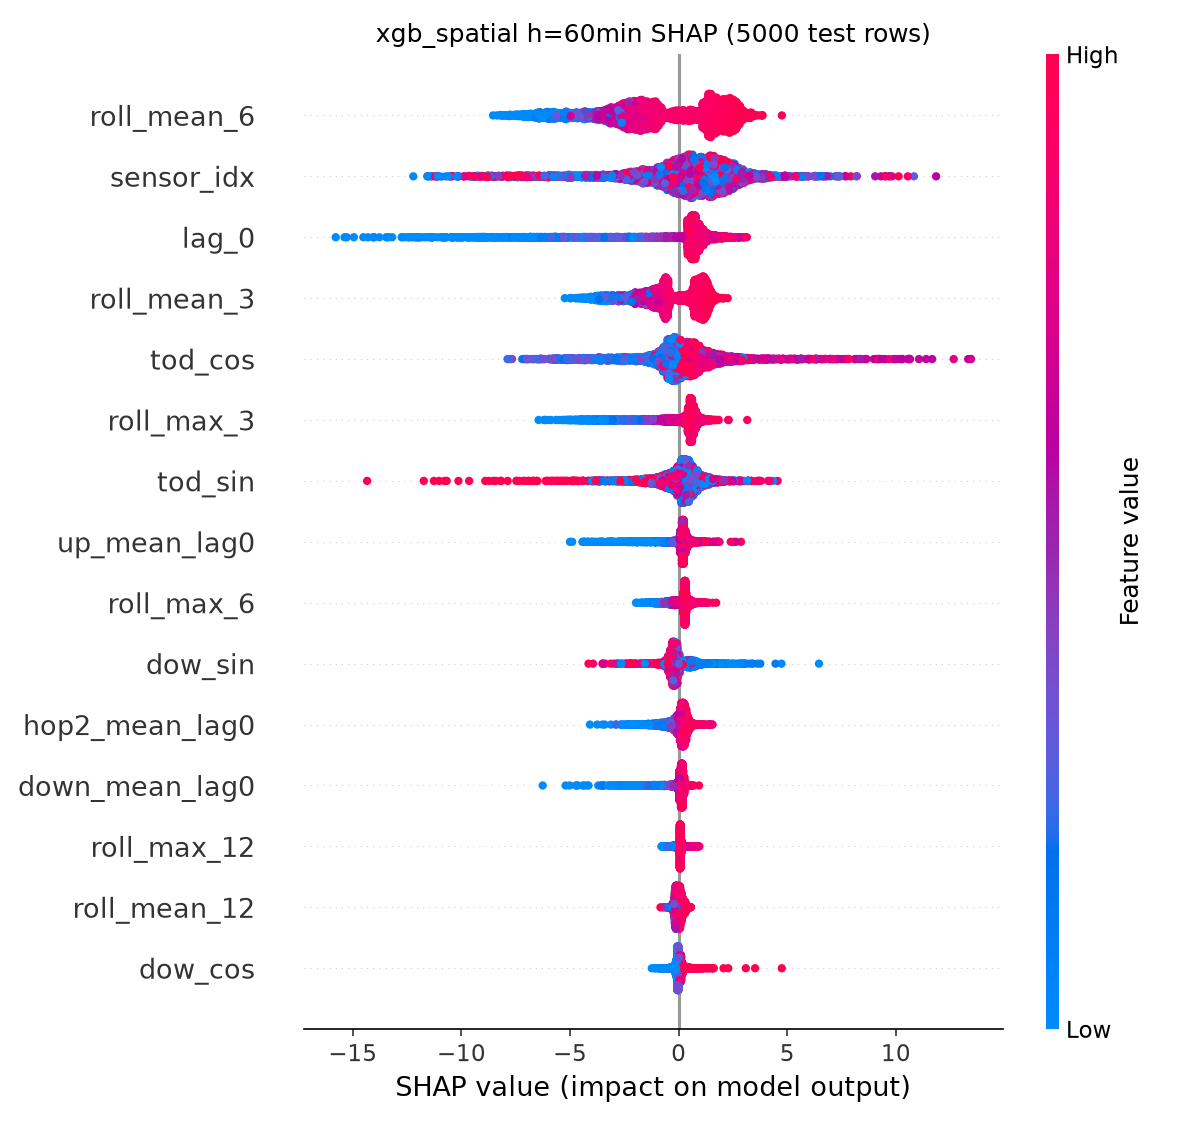
\includegraphics[width=0.83\linewidth]{../../results/figures/ml/shap_xgb_spatial_h12.png}\\[2pt]{\footnotesize\itshape Figure 12. TreeSHAP summary, XGB-spatial at 60 minutes.}\end{figure}

\subsection*{9.7 Gap analysis: what do neighbour features add?}\addcontentsline{toc}{subsection}{9.7 Gap analysis: what do neighbour features add?}
{\scriptsize\renewcommand{\arraystretch}{1.15}\begin{longtable}{>{\raggedright\arraybackslash}p{0.1200\dimexpr\linewidth-14\tabcolsep\relax}>{\raggedright\arraybackslash}p{0.2000\dimexpr\linewidth-14\tabcolsep\relax}>{\raggedright\arraybackslash}p{0.1300\dimexpr\linewidth-14\tabcolsep\relax}>{\raggedright\arraybackslash}p{0.1300\dimexpr\linewidth-14\tabcolsep\relax}>{\raggedright\arraybackslash}p{0.1200\dimexpr\linewidth-14\tabcolsep\relax}>{\raggedright\arraybackslash}p{0.1800\dimexpr\linewidth-14\tabcolsep\relax}>{\raggedright\arraybackslash}p{0.1200\dimexpr\linewidth-14\tabcolsep\relax}}
\toprule
\textbf{Horizon} & \textbf{Slice} & \textbf{MAE global} & \textbf{MAE spatial} & \textbf{\ensuremath{\Delta} MAE} & \textbf{95\% CI} & \textbf{DM p} \\
\midrule
\endhead
\bottomrule
\endlastfoot
15 min & all & 2.880 & 2.820 & +0.059 & [+0.051, +0.069] & 0.000 \\
15 min & peak & 3.866 & 3.749 & +0.117 & [+0.101, +0.135] & 0.000 \\
15 min & offpeak\_\allowbreak{}weekday & 2.579 & 2.540 & +0.038 & [+0.031, +0.048] & 0.000 \\
15 min & weekend & 2.356 & 2.320 & +0.036 & [+0.025, +0.057] & 0.000 \\
15 min & congested & 7.513 & 7.177 & +0.336 & [+0.282, +0.392] & 0.006 \\
15 min & freeflow & 2.226 & 2.205 & +0.020 & [+0.017, +0.024] & 0.000 \\
30 min & all & 3.331 & 3.258 & +0.073 & [+0.059, +0.090] & 0.000 \\
30 min & peak & 4.730 & 4.578 & +0.152 & [+0.126, +0.182] & 0.000 \\
30 min & offpeak\_\allowbreak{}weekday & 2.863 & 2.816 & +0.048 & [+0.034, +0.065] & 0.000 \\
30 min & weekend & 2.697 & 2.661 & +0.037 & [+0.024, +0.057] & 0.000 \\
30 min & congested & 10.147 & 9.588 & +0.559 & [+0.452, +0.670] & 0.000 \\
30 min & freeflow & 2.369 & 2.364 & +0.005 & [-0.003, +0.012] & 0.764 \\
60 min & all & 3.781 & 3.730 & +0.051 & [+0.033, +0.072] & 0.000 \\
60 min & peak & 5.654 & 5.542 & +0.112 & [+0.081, +0.143] & 0.000 \\
60 min & offpeak\_\allowbreak{}weekday & 3.113 & 3.081 & +0.032 & [+0.012, +0.055] & 0.000 \\
60 min & weekend & 3.050 & 3.030 & +0.020 & [+0.000, +0.041] & 0.062 \\
60 min & congested & 13.034 & 12.576 & +0.458 & [+0.343, +0.570] & 0.001 \\
60 min & freeflow & 2.475 & 2.482 & -0.007 & [-0.018, +0.004] & 0.038 \\
\end{longtable}}
{\footnotesize\itshape Table 19. \ensuremath{\Delta} = MAE(global) \ensuremath{-} MAE(spatial); positive means the spatial features help. Paired day-block bootstrap intervals; Diebold--Mariano p-values.}\par\medskip

The spatial features help in almost every slice, most at peaks and in congested states (\ensuremath{\approx} 0.3--0.6 mph in congestion), as the propagation hypothesis predicts --- but the gain does \textbf{not} grow with horizon (largest at 30 minutes), so the ``graph helps more at long horizons'' part is only partly supported. In free flow at 60 minutes they are neutral to slightly harmful.

\begin{figure}[H]\centering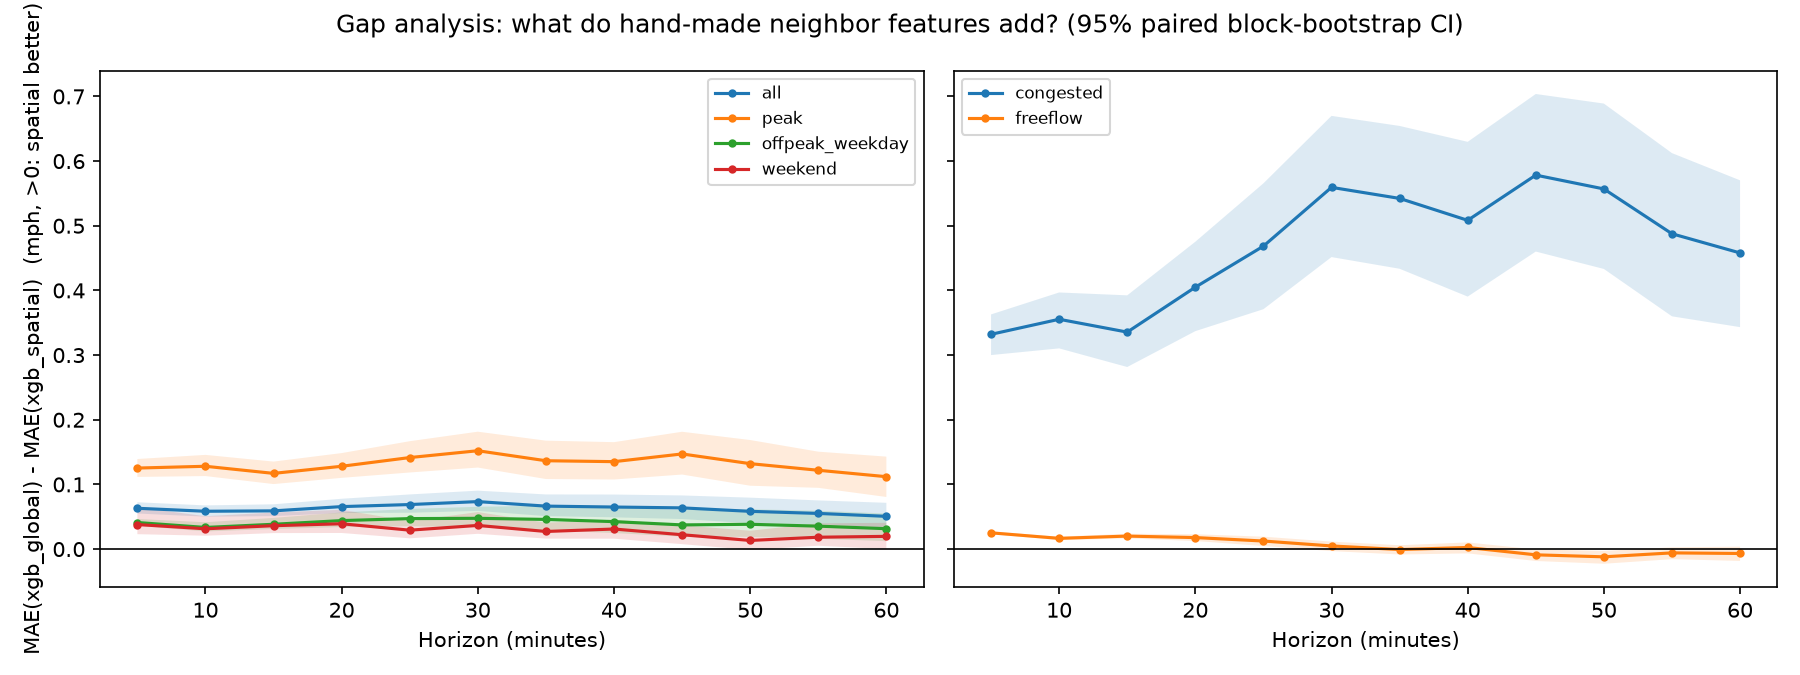
\includegraphics[width=1.00\linewidth]{../../results/figures/ml/gap_analysis.png}\\[2pt]{\footnotesize\itshape Figure 13. Gap analysis by horizon and slice with 95\% intervals.}\end{figure}

\subsection*{9.8 Side experiment: same-time-yesterday lag}\addcontentsline{toc}{subsection}{9.8 Side experiment: same-time-yesterday lag}
{\footnotesize\renewcommand{\arraystretch}{1.15}\begin{longtable}{>{\raggedright\arraybackslash}p{0.4600\dimexpr\linewidth-8\tabcolsep\relax}>{\raggedright\arraybackslash}p{0.1800\dimexpr\linewidth-8\tabcolsep\relax}>{\raggedright\arraybackslash}p{0.1800\dimexpr\linewidth-8\tabcolsep\relax}>{\raggedright\arraybackslash}p{0.1800\dimexpr\linewidth-8\tabcolsep\relax}}
\toprule
\textbf{Model} & \textbf{MAE 15} & \textbf{MAE 30} & \textbf{MAE 60} \\
\midrule
\endhead
\bottomrule
\endlastfoot
XGBoost global (pooled) & 2.8795 & 3.3313 & 3.7805 \\
XGBoost global + daily lag & 2.8788 & 3.3295 & 3.7849 \\
\end{longtable}}
{\footnotesize\itshape Table 20. Adding lag\_\allowbreak{}288 changes nothing material (kept out of the main equal-window comparison).}\par\medskip

\subsection*{9.9 Hardest sensors}\addcontentsline{toc}{subsection}{9.9 Hardest sensors}
{\footnotesize\renewcommand{\arraystretch}{1.15}\begin{longtable}{>{\raggedright\arraybackslash}p{0.2200\dimexpr\linewidth-8\tabcolsep\relax}>{\raggedright\arraybackslash}p{0.2200\dimexpr\linewidth-8\tabcolsep\relax}>{\raggedright\arraybackslash}p{0.2200\dimexpr\linewidth-8\tabcolsep\relax}>{\raggedright\arraybackslash}p{0.3400\dimexpr\linewidth-8\tabcolsep\relax}}
\toprule
\textbf{Sensor} & \textbf{Latitude} & \textbf{Longitude} & \textbf{MAE @ 60 min (XGB global)} \\
\midrule
\endhead
\bottomrule
\endlastfoot
717462 & 34.08993 & -118.30607 & 9.30 \\
717468 & 34.09699 & -118.31381 & 9.03 \\
717466 & 34.09359 & -118.30918 & 9.01 \\
773939 & 34.15297 & -118.37226 & 8.67 \\
717472 & 34.10045 & -118.31601 & 8.61 \\
\end{longtable}}
{\footnotesize\itshape Table 21. The five hardest sensors cluster at one location (\ensuremath{\approx} 34.09 N, 118.31 W).}\par\medskip

\clearpage
\section*{10. Phase 2 --- deep learning}\addcontentsline{toc}{section}{10. Phase 2 --- deep learning}
\subsection*{10.1 The graph attention layer}\addcontentsline{toc}{subsection}{10.1 The graph attention layer}
For node i with neighbourhood N(i) \ensuremath{\cup} \{i\} (self-loops always included), with K heads of size D:

\begin{eqbox}h\ensuremath{'} = W h        e\_\allowbreak{}ij = LeakyReLU( a\_\allowbreak{}dst\ensuremath{^{\top}} h\ensuremath{'}\_\allowbreak{}i + a\_\allowbreak{}src\ensuremath{^{\top}} h\ensuremath{'}\_\allowbreak{}j )  (= a\ensuremath{^{\top}}[h\ensuremath{'}\_\allowbreak{}i \ensuremath{\Vert} h\ensuremath{'}\_\allowbreak{}j])        \ensuremath{\alpha}\_\allowbreak{}ij = softmax\_\allowbreak{}j(e\_\allowbreak{}ij)        out\_\allowbreak{}i = \ensuremath{\Sigma}\_\allowbreak{}j \ensuremath{\alpha}\_\allowbreak{}ij h\ensuremath{'}\_\allowbreak{}j + b\end{eqbox}

\begin{itemize}[nosep,leftmargin=*]
\item \textbf{Dense masked form} (\texttt{DenseGATLayer}): scores for all [N \ensuremath{\times} N] pairs, non-neighbours set to \ensuremath{-}\ensuremath{\infty} before the softmax; heads concatenated (or averaged).
\item \textbf{Sparse form} (\texttt{SparseGATLayer}): padded neighbour lists (D\_\allowbreak{}max = 26 for the bidirectional graph vs N = 207); numerically identical to the dense layer (tested).
\item \textbf{Variants:} GATv2 (dynamic attention, a\ensuremath{^{\top}} LeakyReLU(W\_\allowbreak{}dst h\_\allowbreak{}i + W\_\allowbreak{}src h\_\allowbreak{}j), computed in gradient-checkpointed chunks of 32 graphs), fixed row-normalised weights (``mean'', GCN-style), and an edge-weight bias \ensuremath{\beta}\ensuremath{\cdot}W\_\allowbreak{}ij per head.
\item \textbf{Verification:} outputs and attention weights equal PyTorch Geometric's \texttt{GATConv} (concat and mean) and \texttt{GATv2Conv} within 1e-5 on a random 12-node graph with copied weights (\texttt{tests/\allowbreak{}test\_\allowbreak{}gat\_\allowbreak{}layer.py}). PyG's edge\_\allowbreak{}index is (source j, target i), so it is built as \texttt{adj.nonzero().flip(1).T}.
\end{itemize}

\subsection*{10.2 STGAT architecture}\addcontentsline{toc}{subsection}{10.2 STGAT architecture}
\begin{itemize}[nosep,leftmargin=*]
\item Input X [B, 12, 207, 8] \ensuremath{\rightarrow} Linear 8 \ensuremath{\rightarrow} d = 64 \ensuremath{\rightarrow} plus a learnable node embedding E \ensuremath{\in} \ensuremath{\mathbb{R}}\^{}(207\ensuremath{\times}64).
\item 2 spatio-temporal blocks. Each: gated causal temporal convolution (kernel 3, dilation 1 then 2, GLU gate, left padding so step t sees only \ensuremath{\leq} t) \ensuremath{\rightarrow} multi-head GAT (4 heads \ensuremath{\times} 16 = 64) on the \textbf{last 4 of 12 time steps} \ensuremath{\rightarrow} ELU \ensuremath{\rightarrow} dropout 0.1 \ensuremath{\rightarrow} residual \ensuremath{\rightarrow} LayerNorm.
\item Attention dropout 0.1; graph \texttt{bidirectional} (W + W\ensuremath{^{\top}}); readout = last time step; decoder Linear 64 \ensuremath{\rightarrow} 64 \ensuremath{\rightarrow} ReLU \ensuremath{\rightarrow} dropout \ensuremath{\rightarrow} Linear 64 \ensuremath{\rightarrow} 12.
\item Non-autoregressive: all 12 horizons predicted at once.
\item Parameters: \textbf{77,004}.
\end{itemize}

\subsection*{10.3 GRU no-graph ablation}\addcontentsline{toc}{subsection}{10.3 GRU no-graph ablation}
\begin{itemize}[nosep,leftmargin=*]
\item Same embedding, node embedding, width d = 64, dropout and decoder; a 2-layer GRU runs over each sensor's own 12 steps; no spatial layer.
\item Parameters: \textbf{68,684} (similar capacity), so any gap to STGAT is attributable to the graph, not to deep learning in general.
\end{itemize}

\subsection*{10.4 Training}\addcontentsline{toc}{subsection}{10.4 Training}
{\scriptsize\renewcommand{\arraystretch}{1.15}\begin{longtable}{>{\raggedright\arraybackslash}p{0.2800\dimexpr\linewidth-4\tabcolsep\relax}>{\raggedright\arraybackslash}p{0.7200\dimexpr\linewidth-4\tabcolsep\relax}}
\toprule
\textbf{Setting} & \textbf{Value} \\
\midrule
\endhead
\bottomrule
\endlastfoot
Loss & masked MAE in scaled space (normalised by the number of observed targets) \\
Optimiser & Adam, learning rate 0.001, weight decay 0.0001 \\
Schedule & ReduceLROnPlateau on validation MAE (factor 0.5, patience 5) \\
Gradient clipping & norm 5.0 \\
Batch size & 64 \\
Epochs & max 40, early stopping patience 8 on validation MAE in mph; best weights restored \\
Epoch fraction & 0.34 (each epoch sees a random third of the training windows) \\
Seeds & 0, 1, 2 \\
Device & Apple M3 Pro GPU (PyTorch MPS), 4 CPU threads, low priority \\
\end{longtable}}
{\footnotesize\itshape Table 22. Deep-learning training configuration (same for STGAT and GRU).}\par\medskip

\subsection*{10.5 Compute study and simplification (ADR-007)}\addcontentsline{toc}{subsection}{10.5 Compute study and simplification (ADR-007)}
{\scriptsize\renewcommand{\arraystretch}{1.15}\begin{longtable}{>{\raggedright\arraybackslash}p{0.5600\dimexpr\linewidth-6\tabcolsep\relax}>{\raggedright\arraybackslash}p{0.2000\dimexpr\linewidth-6\tabcolsep\relax}>{\raggedright\arraybackslash}p{0.2400\dimexpr\linewidth-6\tabcolsep\relax}}
\toprule
\textbf{Configuration} & \textbf{Time per iteration} & \textbf{Time per epoch} \\
\midrule
\endhead
\bottomrule
\endlastfoot
STGAT dense, GAT on all 12 steps, CPU & 4.34 s & 27.1 min \\
STGAT dense, GAT on all 12 steps, MPS & 0.59 s & 3.7 min \\
STGAT sparse neighbour lists, all 12 steps, MPS & 0.66 s & 4.1 min (no gain: gathers dominate) \\
STGAT GAT on last 4 steps + 34\% of windows per epoch, MPS & 0.28 s & \ensuremath{\approx} 0.6 min (+ validation) \\
GRU no-graph, CPU /\allowbreak{} MPS (full epoch) & 0.27 s /\allowbreak{} 0.08 s & 1.7 /\allowbreak{} 0.5 min \\
\end{longtable}}
{\footnotesize\itshape Table 23. Measured training speed that motivated the simplification.}\par\medskip

Profiling showed the per-block cost was dominated by the graph attention (0.26 s of 0.33 s per block), which is memory-bound. Applying attention on the most recent 4 steps (20 minutes of neighbour state) and sampling a third of the highly redundant windows each epoch cut the cost about six-fold, to \ensuremath{\approx} 28 minutes per seed.

\subsection*{10.6 Training outcomes}\addcontentsline{toc}{subsection}{10.6 Training outcomes}
{\scriptsize\renewcommand{\arraystretch}{1.15}\begin{longtable}{>{\raggedright\arraybackslash}p{0.2600\dimexpr\linewidth-12\tabcolsep\relax}>{\raggedright\arraybackslash}p{0.0900\dimexpr\linewidth-12\tabcolsep\relax}>{\raggedright\arraybackslash}p{0.1400\dimexpr\linewidth-12\tabcolsep\relax}>{\raggedright\arraybackslash}p{0.1400\dimexpr\linewidth-12\tabcolsep\relax}>{\raggedright\arraybackslash}p{0.2100\dimexpr\linewidth-12\tabcolsep\relax}>{\raggedright\arraybackslash}p{0.1600\dimexpr\linewidth-12\tabcolsep\relax}}
\toprule
\textbf{Model} & \textbf{Seed} & \textbf{Epochs run} & \textbf{Best epoch} & \textbf{Best val MAE (mph)} & \textbf{Train time} \\
\midrule
\endhead
\bottomrule
\endlastfoot
GRU no-graph & 0 & 40 & 34 & 3.0136 & 490 s \\
GRU no-graph & 1 & 40 & 40 & 3.0088 & 496 s \\
GRU no-graph & 2 & 33 & 25 & 3.0162 & 413 s \\
STGAT & 0 & 40 & 40 & 2.9817 & 1692 s \\
STGAT & 1 & 40 & 40 & 2.9947 & 1685 s \\
STGAT & 2 & 40 & 35 & 2.9802 & 1687 s \\
Hybrid: residual & 0 & 40 & 40 & 2.9312 & 1391 s \\
Hybrid: residual & 1 & 40 & 32 & 2.9332 & 1379 s \\
Hybrid: residual & 2 & 40 & 40 & 2.9335 & 1383 s \\
\end{longtable}}
{\footnotesize\itshape Table 24. Per-seed training results. STGAT never triggered early stopping within 40 epochs (it was still improving).}\par\medskip

\begin{figure}[H]\centering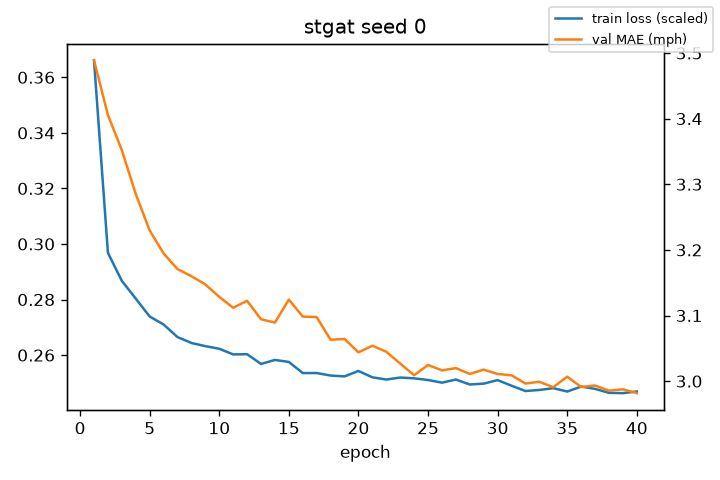
\includegraphics[width=0.73\linewidth]{../../results/figures/training/stgat_seed0.png}\\[2pt]{\footnotesize\itshape Figure 14. Training curve, STGAT seed 0 (training loss in scaled units; validation MAE in mph).}\end{figure}

\subsection*{10.7 Results}\addcontentsline{toc}{subsection}{10.7 Results}
{\scriptsize\renewcommand{\arraystretch}{1.15}\begin{longtable}{>{\raggedright\arraybackslash}p{0.1429\dimexpr\linewidth-14\tabcolsep\relax}>{\raggedright\arraybackslash}p{0.1429\dimexpr\linewidth-14\tabcolsep\relax}>{\raggedright\arraybackslash}p{0.1429\dimexpr\linewidth-14\tabcolsep\relax}>{\raggedright\arraybackslash}p{0.1429\dimexpr\linewidth-14\tabcolsep\relax}>{\raggedright\arraybackslash}p{0.1429\dimexpr\linewidth-14\tabcolsep\relax}>{\raggedright\arraybackslash}p{0.1429\dimexpr\linewidth-14\tabcolsep\relax}>{\raggedright\arraybackslash}p{0.1429\dimexpr\linewidth-14\tabcolsep\relax}}
\toprule
\textbf{Model} & \textbf{MAE 15} & \textbf{MAE 30} & \textbf{MAE 60} & \textbf{RMSE 15} & \textbf{RMSE 30} & \textbf{RMSE 60} \\
\midrule
\endhead
\bottomrule
\endlastfoot
XGBoost per-segment & 2.860 & 3.276 & 3.684 & 5.601 & 6.616 & 7.516 \\
XGBoost global (pooled) & 2.880 & 3.331 & 3.781 & 5.691 & 6.801 & 7.762 \\
XGBoost spatial & 2.820 & 3.258 & 3.730 & 5.465 & 6.544 & 7.544 \\
GRU no-graph & 2.892 \ensuremath{\pm} 0.007 & 3.313 \ensuremath{\pm} 0.013 & 3.761 \ensuremath{\pm} 0.036 & 5.618 \ensuremath{\pm} 0.032 & 6.655 \ensuremath{\pm} 0.036 & 7.710 \ensuremath{\pm} 0.095 \\
STGAT & 2.901 \ensuremath{\pm} 0.011 & 3.276 \ensuremath{\pm} 0.021 & 3.666 \ensuremath{\pm} 0.022 & 5.524 \ensuremath{\pm} 0.010 & 6.483 \ensuremath{\pm} 0.007 & 7.436 \ensuremath{\pm} 0.072 \\
\end{longtable}}
{\footnotesize\itshape Table 25. Deep models vs the tree models (mph; \ensuremath{\pm} std over 3 seeds).}\par\medskip

\begin{itemize}[nosep,leftmargin=*]
\item STGAT beats persistence at every horizon (acceptance criterion met).
\item Graph vs no graph: equal at 15 minutes (2.901 vs 2.892, DM not significant), slightly ahead at 30 (3.276 vs 3.313, not significant), clearly ahead at 60 (3.666 vs 3.761, significant).
\item Deep vs trees: STGAT is slightly worse than pooled XGBoost at 15 minutes (2.901 vs 2.880) and better at 60 (3.666 vs 3.781); per-segment XGBoost stays very close at 60 minutes (3.684).
\item STGAT has a lower RMSE than every tree model at 30 and 60 minutes, i.e. fewer large misses.
\end{itemize}

\clearpage
\section*{11. Hybrid models}\addcontentsline{toc}{section}{11. Hybrid models}
\subsection*{11.1 Why a residual hybrid}\addcontentsline{toc}{subsection}{11.1 Why a residual hybrid}
XGBoost captures local autoregression and calendar effects cheaply; spatial propagation is its blind spot. The residual hybrid trains STGAT to learn only what XGBoost misses:

\begin{eqbox}\ensuremath{\hat{y}}\_\allowbreak{}hybrid(t + h, i) = \ensuremath{\hat{y}}\_\allowbreak{}XGB(t + h, i) + g\_\allowbreak{}\ensuremath{\theta}(X\_\allowbreak{}window, \ensuremath{\hat{y}}\_\allowbreak{}XGB, G)(h, i)\end{eqbox}

STGAT receives the scaled XGBoost forecast (12 values per sensor) concatenated to its readout before the decoder, and the last decoder layer is zero-initialised, so training starts exactly at the XGBoost forecast (tested).

\subsection*{11.2 Leakage-safe out-of-fold base forecasts}\addcontentsline{toc}{subsection}{11.2 Leakage-safe out-of-fold base forecasts}
\begin{itemize}[nosep,leftmargin=*]
\item XGBoost's predictions on its own training rows are overfit; their residuals are unrealistically small. The residual model must learn from \textbf{out-of-fold (OOF)} forecasts instead.
\item Forward-chaining over the 23,967 training windows in 5 chronological blocks with edges [0, 4793, 9586, 14380, 19173, 23967].
\item For blocks 2--5, an XGBoost model (tuned global parameters, 15\% row sample, early stopping on 20,000 validation rows) trained on the earlier blocks predicts the block; a gap of H + F \ensuremath{-} 1 = 23 anchors separates training targets from the block's inputs.
\item Block 1 gets no OOF forecast and is dropped: residual training uses 19,174 windows (80.0\% coverage).
\item The final XGBoost models (trained on all training rows) provide the base forecasts for validation and test.
\item Caveat: early-block models see less data, so OOF errors are slightly larger than the final model's --- the conservative direction.
\end{itemize}

\subsection*{11.3 Gating ensemble and simple average}\addcontentsline{toc}{subsection}{11.3 Gating ensemble and simple average}
\begin{itemize}[nosep,leftmargin=*]
\item \textbf{Gate:} \ensuremath{\hat{y}} = w\ensuremath{\cdot}\ensuremath{\hat{y}}\_\allowbreak{}STGAT + (1 \ensuremath{-} w)\ensuremath{\cdot}\ensuremath{\hat{y}}\_\allowbreak{}XGB with w = sigmoid(MLP(16 \ensuremath{\rightarrow} 16 \ensuremath{\rightarrow} 1)) of horizon one-hot (12), weekday-peak flag, time-of-day sin/\allowbreak{}cos of the target, and the input window's missing rate; trained with Adam (lr 0.01) on the first 80\% of validation windows, early-stopped (patience 30, \ensuremath{\leq} 400 steps) on the last 20\% (ADR-008: validation is then not fully independent).
\item \textbf{Average:} 0.5\ensuremath{\cdot}\ensuremath{\hat{y}}\_\allowbreak{}XGB + 0.5\ensuremath{\cdot}\ensuremath{\hat{y}}\_\allowbreak{}STGAT, per seed.
\item All hybrids: 3 seeds, paired with the STGAT seed.
\end{itemize}

\subsection*{11.4 Results}\addcontentsline{toc}{subsection}{11.4 Results}
{\scriptsize\renewcommand{\arraystretch}{1.15}\begin{longtable}{>{\raggedright\arraybackslash}p{0.1429\dimexpr\linewidth-14\tabcolsep\relax}>{\raggedright\arraybackslash}p{0.1429\dimexpr\linewidth-14\tabcolsep\relax}>{\raggedright\arraybackslash}p{0.1429\dimexpr\linewidth-14\tabcolsep\relax}>{\raggedright\arraybackslash}p{0.1429\dimexpr\linewidth-14\tabcolsep\relax}>{\raggedright\arraybackslash}p{0.1429\dimexpr\linewidth-14\tabcolsep\relax}>{\raggedright\arraybackslash}p{0.1429\dimexpr\linewidth-14\tabcolsep\relax}>{\raggedright\arraybackslash}p{0.1429\dimexpr\linewidth-14\tabcolsep\relax}}
\toprule
\textbf{Model} & \textbf{MAE 15} & \textbf{MAE 30} & \textbf{MAE 60} & \textbf{RMSE 15} & \textbf{RMSE 30} & \textbf{RMSE 60} \\
\midrule
\endhead
\bottomrule
\endlastfoot
XGBoost global (pooled) & 2.880 & 3.331 & 3.781 & 5.691 & 6.801 & 7.762 \\
STGAT & 2.901 \ensuremath{\pm} 0.011 & 3.276 \ensuremath{\pm} 0.021 & 3.666 \ensuremath{\pm} 0.022 & 5.524 \ensuremath{\pm} 0.010 & 6.483 \ensuremath{\pm} 0.007 & 7.436 \ensuremath{\pm} 0.072 \\
Hybrid: residual & 2.820 \ensuremath{\pm} 0.005 & 3.219 \ensuremath{\pm} 0.002 & 3.647 \ensuremath{\pm} 0.009 & 5.461 \ensuremath{\pm} 0.029 & 6.453 \ensuremath{\pm} 0.033 & 7.456 \ensuremath{\pm} 0.021 \\
Hybrid: gating & 2.836 \ensuremath{\pm} 0.005 & 3.233 \ensuremath{\pm} 0.012 & 3.607 \ensuremath{\pm} 0.018 & 5.522 \ensuremath{\pm} 0.008 & 6.448 \ensuremath{\pm} 0.012 & 7.344 \ensuremath{\pm} 0.063 \\
Hybrid: average & 2.840 \ensuremath{\pm} 0.005 & 3.246 \ensuremath{\pm} 0.010 & 3.640 \ensuremath{\pm} 0.018 & 5.525 \ensuremath{\pm} 0.007 & 6.506 \ensuremath{\pm} 0.013 & 7.392 \ensuremath{\pm} 0.058 \\
\end{longtable}}
{\footnotesize\itshape Table 26. Hybrids vs their components (mph; \ensuremath{\pm} std over 3 seeds).}\par\medskip

{\scriptsize\renewcommand{\arraystretch}{1.15}\begin{longtable}{>{\raggedright\arraybackslash}p{0.3000\dimexpr\linewidth-10\tabcolsep\relax}>{\raggedright\arraybackslash}p{0.2200\dimexpr\linewidth-10\tabcolsep\relax}>{\raggedright\arraybackslash}p{0.1600\dimexpr\linewidth-10\tabcolsep\relax}>{\raggedright\arraybackslash}p{0.1600\dimexpr\linewidth-10\tabcolsep\relax}>{\raggedright\arraybackslash}p{0.1600\dimexpr\linewidth-10\tabcolsep\relax}}
\toprule
\textbf{Component} & \textbf{Slice} & \textbf{Gain 15} & \textbf{Gain 30} & \textbf{Gain 60} \\
\midrule
\endhead
\bottomrule
\endlastfoot
STGAT & all & +0.081 & +0.058 & +0.019 \\
STGAT & peak & +0.106 & +0.084 & -0.091 \\
STGAT & offpeak\_\allowbreak{}weekday & +0.073 & +0.047 & +0.056 \\
STGAT & weekend & +0.069 & +0.049 & +0.064 \\
STGAT & congested & +0.258 & +0.327 & -0.591 \\
STGAT & freeflow & +0.056 & +0.020 & +0.105 \\
XGBoost global (pooled) & all & +0.059 & +0.113 & +0.133 \\
XGBoost global (pooled) & peak & +0.146 & +0.304 & +0.374 \\
XGBoost global (pooled) & offpeak\_\allowbreak{}weekday & +0.027 & +0.041 & +0.037 \\
XGBoost global (pooled) & weekend & +0.027 & +0.046 & +0.066 \\
XGBoost global (pooled) & congested & +0.609 & +1.283 & +1.536 \\
XGBoost global (pooled) & freeflow & -0.018 & -0.052 & -0.065 \\
\end{longtable}}
{\footnotesize\itshape Table 27. Gain of the residual hybrid = MAE(component) \ensuremath{-} MAE(hybrid), seed-averaged (positive: hybrid better).}\par\medskip

Over XGBoost the residual hybrid's gain grows with horizon and is largest in congestion and at peaks; in free flow at 60 minutes it is slightly negative. Over STGAT the gain shrinks with horizon: STGAT already captures much of the local structure at long range.

{\scriptsize\renewcommand{\arraystretch}{1.15}\begin{longtable}{>{\raggedright\arraybackslash}p{0.0769\dimexpr\linewidth-26\tabcolsep\relax}>{\raggedright\arraybackslash}p{0.0769\dimexpr\linewidth-26\tabcolsep\relax}>{\raggedright\arraybackslash}p{0.0769\dimexpr\linewidth-26\tabcolsep\relax}>{\raggedright\arraybackslash}p{0.0769\dimexpr\linewidth-26\tabcolsep\relax}>{\raggedright\arraybackslash}p{0.0769\dimexpr\linewidth-26\tabcolsep\relax}>{\raggedright\arraybackslash}p{0.0769\dimexpr\linewidth-26\tabcolsep\relax}>{\raggedright\arraybackslash}p{0.0769\dimexpr\linewidth-26\tabcolsep\relax}>{\raggedright\arraybackslash}p{0.0769\dimexpr\linewidth-26\tabcolsep\relax}>{\raggedright\arraybackslash}p{0.0769\dimexpr\linewidth-26\tabcolsep\relax}>{\raggedright\arraybackslash}p{0.0769\dimexpr\linewidth-26\tabcolsep\relax}>{\raggedright\arraybackslash}p{0.0769\dimexpr\linewidth-26\tabcolsep\relax}>{\raggedright\arraybackslash}p{0.0769\dimexpr\linewidth-26\tabcolsep\relax}>{\raggedright\arraybackslash}p{0.0769\dimexpr\linewidth-26\tabcolsep\relax}}
\toprule
\textbf{Horizon (min)} & \textbf{5} & \textbf{10} & \textbf{15} & \textbf{20} & \textbf{25} & \textbf{30} & \textbf{35} & \textbf{40} & \textbf{45} & \textbf{50} & \textbf{55} & \textbf{60} \\
\midrule
\endhead
\bottomrule
\endlastfoot
Weight on STGAT, peak & 0.35 & 0.49 & 0.56 & 0.65 & 0.72 & 0.79 & 0.82 & 0.85 & 0.85 & 0.84 & 0.82 & 0.79 \\
Weight on STGAT, off-peak & 0.18 & 0.27 & 0.33 & 0.36 & 0.40 & 0.45 & 0.49 & 0.50 & 0.52 & 0.49 & 0.45 & 0.42 \\
\end{longtable}}
{\footnotesize\itshape Table 28. Mean learned gate weight on STGAT (test set, averaged over seeds).}\par\medskip

The gate trusts STGAT more at peaks than off-peak and more at longer horizons --- exactly the pattern the hypothesis predicts.

\begin{figure}[H]\centering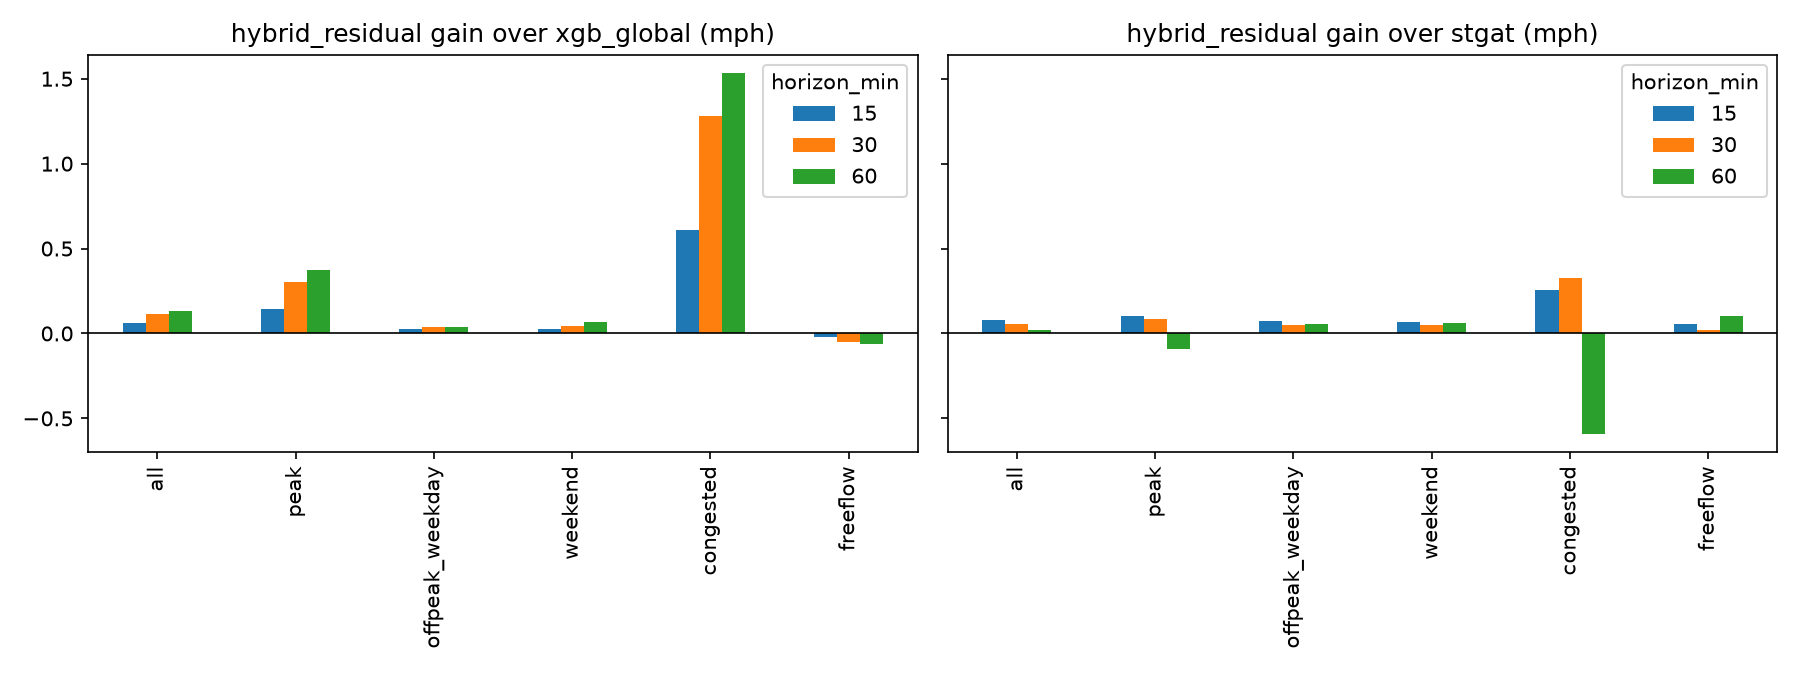
\includegraphics[width=1.00\linewidth]{../../results/figures/hybrid/hybrid_gain.png}\\[2pt]{\footnotesize\itshape Figure 15. Residual-hybrid gain over XGBoost-global and over STGAT by slice and horizon.}\end{figure}

\begin{figure}[H]\centering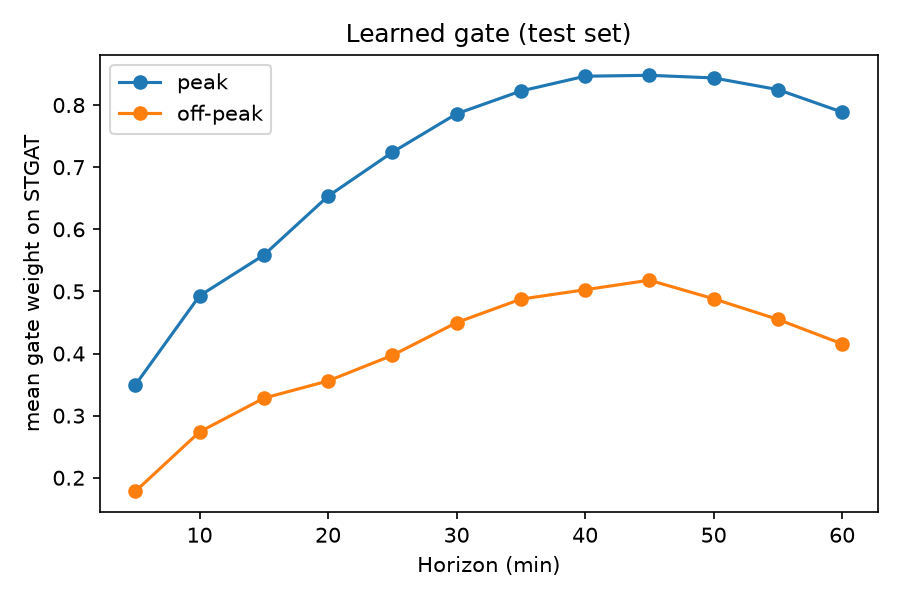
\includegraphics[width=0.70\linewidth]{../../results/figures/hybrid/gate_weights.png}\\[2pt]{\footnotesize\itshape Figure 16. Learned gate weight on STGAT by horizon, peak vs off-peak.}\end{figure}

\clearpage
\section*{12. All results}\addcontentsline{toc}{section}{12. All results}
\subsection*{12.1 Main table}\addcontentsline{toc}{subsection}{12.1 Main table}
{\scriptsize\renewcommand{\arraystretch}{1.15}\begin{longtable}{>{\raggedright\arraybackslash}p{0.1000\dimexpr\linewidth-20\tabcolsep\relax}>{\raggedright\arraybackslash}p{0.1000\dimexpr\linewidth-20\tabcolsep\relax}>{\raggedright\arraybackslash}p{0.1000\dimexpr\linewidth-20\tabcolsep\relax}>{\raggedright\arraybackslash}p{0.1000\dimexpr\linewidth-20\tabcolsep\relax}>{\raggedright\arraybackslash}p{0.1000\dimexpr\linewidth-20\tabcolsep\relax}>{\raggedright\arraybackslash}p{0.1000\dimexpr\linewidth-20\tabcolsep\relax}>{\raggedright\arraybackslash}p{0.1000\dimexpr\linewidth-20\tabcolsep\relax}>{\raggedright\arraybackslash}p{0.1000\dimexpr\linewidth-20\tabcolsep\relax}>{\raggedright\arraybackslash}p{0.1000\dimexpr\linewidth-20\tabcolsep\relax}>{\raggedright\arraybackslash}p{0.1000\dimexpr\linewidth-20\tabcolsep\relax}}
\toprule
\textbf{Model} & \textbf{MAE 15} & \textbf{MAE 30} & \textbf{MAE 60} & \textbf{RMSE 15} & \textbf{RMSE 30} & \textbf{RMSE 60} & \textbf{MAPE 15} & \textbf{MAPE 30} & \textbf{MAPE 60} \\
\midrule
\endhead
\bottomrule
\endlastfoot
Persistence & 3.494 & 4.198 & 5.368 & 6.394 & 8.016 & 10.296 & 8.597 & 10.826 & 14.479 \\
Historical average & 4.193 & 4.193 & 4.193 & 7.862 & 7.862 & 7.862 & 13.059 & 13.059 & 13.059 \\
Seasonal naive & 5.503 & 5.503 & 5.503 & 10.711 & 10.711 & 10.711 & 15.573 & 15.573 & 15.573 \\
XGBoost per-segment & 2.860 & 3.276 & 3.684 & 5.601 & 6.616 & 7.516 & 7.916 & 9.773 & 11.652 \\
XGBoost global (pooled) & 2.880 & 3.331 & 3.781 & 5.691 & 6.801 & 7.762 & 7.871 & 9.899 & 12.112 \\
Random Forest (multi-output) & 3.137 & 3.798 & 4.732 & 5.704 & 6.892 & 8.251 & 8.501 & 10.875 & 14.268 \\
XGBoost spatial & 2.820 & 3.258 & 3.730 & 5.465 & 6.544 & 7.544 & 7.633 & 9.526 & 11.818 \\
GRU no-graph & 2.892 & 3.313 & 3.761 & 5.618 & 6.655 & 7.710 & 7.835 & 9.670 & 11.533 \\
STGAT & 2.901 & 3.276 & 3.666 & 5.524 & 6.483 & 7.436 & 7.765 & 9.407 & 10.970 \\
Hybrid: residual & 2.820 & 3.219 & 3.647 & 5.461 & 6.453 & 7.456 & 7.507 & 9.184 & 11.217 \\
Hybrid: gating & 2.836 & 3.233 & 3.607 & 5.522 & 6.448 & 7.344 & 7.677 & 9.383 & 11.029 \\
Hybrid: average & 2.840 & 3.246 & 3.640 & 5.525 & 6.506 & 7.392 & 7.694 & 9.512 & 11.323 \\
\end{longtable}}
{\footnotesize\itshape Table 29. All models, all headline metrics (seed means for deep models).}\par\medskip

\begin{figure}[H]\centering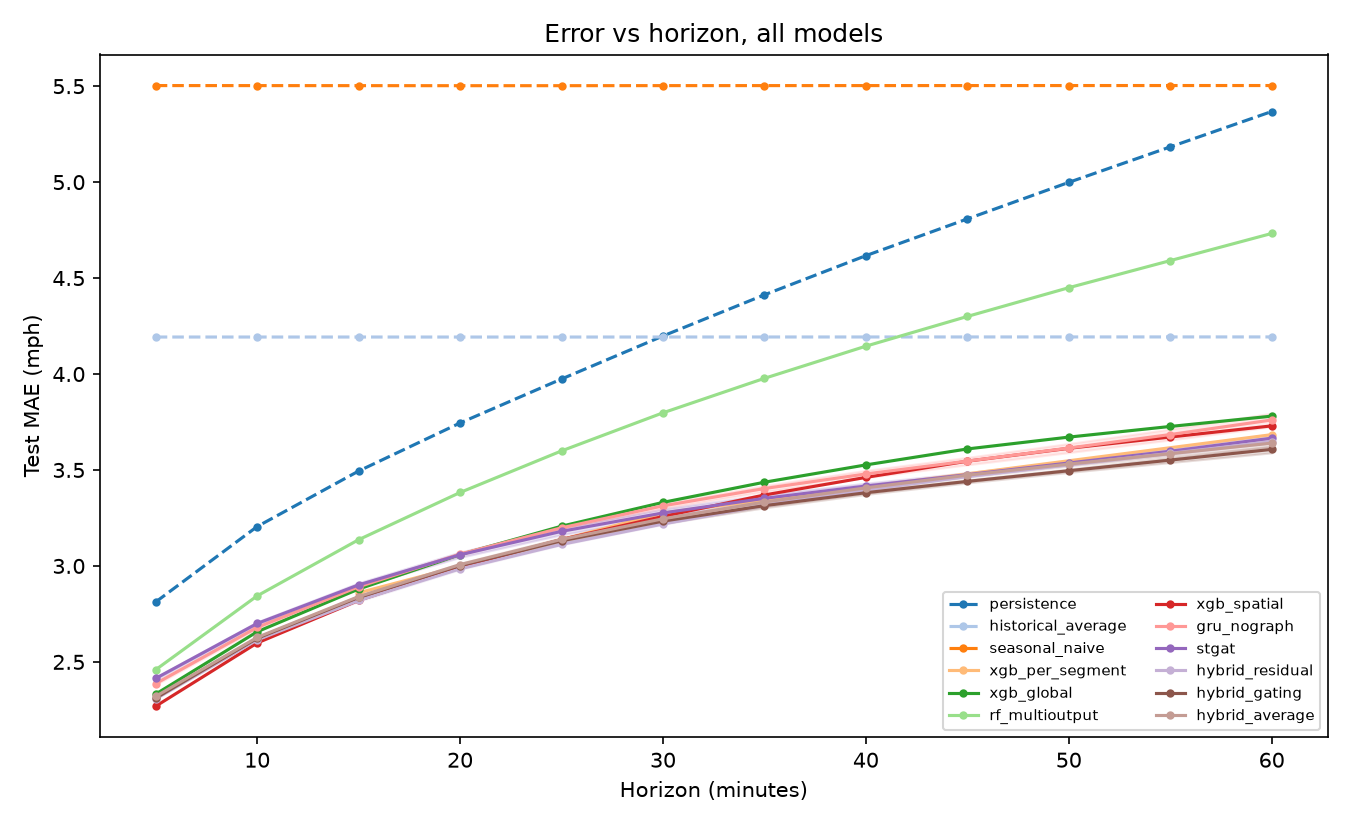
\includegraphics[width=1.00\linewidth]{../../results/figures/error_vs_horizon_all_models.png}\\[2pt]{\footnotesize\itshape Figure 17. MAE vs horizon for every model (bands: \ensuremath{\pm} std over seeds).}\end{figure}

\subsection*{12.2 Every horizon}\addcontentsline{toc}{subsection}{12.2 Every horizon}
{\scriptsize\renewcommand{\arraystretch}{1.15}\begin{longtable}{>{\raggedright\arraybackslash}p{0.0769\dimexpr\linewidth-26\tabcolsep\relax}>{\raggedright\arraybackslash}p{0.0769\dimexpr\linewidth-26\tabcolsep\relax}>{\raggedright\arraybackslash}p{0.0769\dimexpr\linewidth-26\tabcolsep\relax}>{\raggedright\arraybackslash}p{0.0769\dimexpr\linewidth-26\tabcolsep\relax}>{\raggedright\arraybackslash}p{0.0769\dimexpr\linewidth-26\tabcolsep\relax}>{\raggedright\arraybackslash}p{0.0769\dimexpr\linewidth-26\tabcolsep\relax}>{\raggedright\arraybackslash}p{0.0769\dimexpr\linewidth-26\tabcolsep\relax}>{\raggedright\arraybackslash}p{0.0769\dimexpr\linewidth-26\tabcolsep\relax}>{\raggedright\arraybackslash}p{0.0769\dimexpr\linewidth-26\tabcolsep\relax}>{\raggedright\arraybackslash}p{0.0769\dimexpr\linewidth-26\tabcolsep\relax}>{\raggedright\arraybackslash}p{0.0769\dimexpr\linewidth-26\tabcolsep\relax}>{\raggedright\arraybackslash}p{0.0769\dimexpr\linewidth-26\tabcolsep\relax}>{\raggedright\arraybackslash}p{0.0769\dimexpr\linewidth-26\tabcolsep\relax}}
\toprule
\textbf{Model} & \textbf{5} & \textbf{10} & \textbf{15} & \textbf{20} & \textbf{25} & \textbf{30} & \textbf{35} & \textbf{40} & \textbf{45} & \textbf{50} & \textbf{55} & \textbf{60} \\
\midrule
\endhead
\bottomrule
\endlastfoot
Persistence & 2.81 & 3.21 & 3.49 & 3.74 & 3.97 & 4.20 & 4.41 & 4.62 & 4.81 & 5.00 & 5.18 & 5.37 \\
Historical average & 4.19 & 4.19 & 4.19 & 4.19 & 4.19 & 4.19 & 4.19 & 4.19 & 4.19 & 4.19 & 4.19 & 4.19 \\
Seasonal naive & 5.50 & 5.50 & 5.50 & 5.50 & 5.50 & 5.50 & 5.50 & 5.50 & 5.50 & 5.50 & 5.50 & 5.50 \\
XGBoost per-segment & -- & -- & 2.86 & -- & -- & 3.28 & -- & -- & -- & -- & -- & 3.68 \\
XGBoost global (pooled) & 2.33 & 2.66 & 2.88 & 3.06 & 3.21 & 3.33 & 3.44 & 3.53 & 3.61 & 3.67 & 3.73 & 3.78 \\
Random Forest (multi-output) & 2.46 & 2.84 & 3.14 & 3.38 & 3.60 & 3.80 & 3.98 & 4.15 & 4.30 & 4.45 & 4.59 & 4.73 \\
XGBoost spatial & 2.27 & 2.60 & 2.82 & 2.99 & 3.14 & 3.26 & 3.37 & 3.46 & 3.55 & 3.61 & 3.67 & 3.73 \\
GRU no-graph & 2.39 & 2.68 & 2.89 & 3.06 & 3.20 & 3.31 & 3.40 & 3.48 & 3.55 & 3.61 & 3.68 & 3.76 \\
STGAT & 2.41 & 2.70 & 2.90 & 3.06 & 3.18 & 3.28 & 3.35 & 3.42 & 3.48 & 3.54 & 3.60 & 3.67 \\
Hybrid: residual & 2.31 & 2.61 & 2.82 & 2.98 & 3.11 & 3.22 & 3.32 & 3.40 & 3.47 & 3.53 & 3.59 & 3.65 \\
Hybrid: gating & 2.31 & 2.62 & 2.84 & 3.00 & 3.13 & 3.23 & 3.31 & 3.38 & 3.44 & 3.50 & 3.55 & 3.61 \\
Hybrid: average & 2.32 & 2.63 & 2.84 & 3.01 & 3.14 & 3.25 & 3.33 & 3.41 & 3.47 & 3.53 & 3.58 & 3.64 \\
\end{longtable}}
{\footnotesize\itshape Table 30. MAE (mph) at every horizon in minutes.}\par\medskip

\subsection*{12.3 Peak, off-peak and weekend}\addcontentsline{toc}{subsection}{12.3 Peak, off-peak and weekend}
{\scriptsize\renewcommand{\arraystretch}{1.15}\begin{longtable}{>{\raggedright\arraybackslash}p{0.1429\dimexpr\linewidth-14\tabcolsep\relax}>{\raggedright\arraybackslash}p{0.1429\dimexpr\linewidth-14\tabcolsep\relax}>{\raggedright\arraybackslash}p{0.1429\dimexpr\linewidth-14\tabcolsep\relax}>{\raggedright\arraybackslash}p{0.1429\dimexpr\linewidth-14\tabcolsep\relax}>{\raggedright\arraybackslash}p{0.1429\dimexpr\linewidth-14\tabcolsep\relax}>{\raggedright\arraybackslash}p{0.1429\dimexpr\linewidth-14\tabcolsep\relax}>{\raggedright\arraybackslash}p{0.1429\dimexpr\linewidth-14\tabcolsep\relax}}
\toprule
\textbf{Model} & \textbf{Peak 15} & \textbf{Peak 60} & \textbf{Off-peak 15} & \textbf{Off-peak 60} & \textbf{Weekend 15} & \textbf{Weekend 60} \\
\midrule
\endhead
\bottomrule
\endlastfoot
Persistence & 4.39 & 7.45 & 3.29 & 4.85 & 2.86 & 3.98 \\
Historical average & 6.04 & 6.06 & 3.52 & 3.51 & 3.50 & 3.50 \\
Seasonal naive & 7.45 & 7.48 & 4.38 & 4.37 & 5.83 & 5.83 \\
XGBoost per-segment & 3.78 & 5.26 & 2.57 & 3.11 & 2.38 & 3.09 \\
XGBoost global (pooled) & 3.87 & 5.65 & 2.58 & 3.11 & 2.36 & 3.05 \\
Random Forest (multi-output) & 4.21 & 7.24 & 2.80 & 3.82 & 2.59 & 3.80 \\
XGBoost spatial & 3.75 & 5.54 & 2.54 & 3.08 & 2.32 & 3.03 \\
GRU no-graph & 3.84 & 5.43 & 2.60 & 3.18 & 2.39 & 3.07 \\
STGAT & 3.83 & 5.19 & 2.62 & 3.13 & 2.40 & 3.05 \\
Hybrid: residual & 3.72 & 5.28 & 2.55 & 3.08 & 2.33 & 2.98 \\
Hybrid: gating & 3.76 & 5.14 & 2.56 & 3.07 & 2.33 & 2.99 \\
Hybrid: average & 3.77 & 5.25 & 2.56 & 3.07 & 2.34 & 3.00 \\
\end{longtable}}
{\footnotesize\itshape Table 31. MAE by time slice (mph).}\par\medskip

\subsection*{12.4 Congested vs free-flow}\addcontentsline{toc}{subsection}{12.4 Congested vs free-flow}
{\scriptsize\renewcommand{\arraystretch}{1.15}\begin{longtable}{>{\raggedright\arraybackslash}p{0.1429\dimexpr\linewidth-14\tabcolsep\relax}>{\raggedright\arraybackslash}p{0.1429\dimexpr\linewidth-14\tabcolsep\relax}>{\raggedright\arraybackslash}p{0.1429\dimexpr\linewidth-14\tabcolsep\relax}>{\raggedright\arraybackslash}p{0.1429\dimexpr\linewidth-14\tabcolsep\relax}>{\raggedright\arraybackslash}p{0.1429\dimexpr\linewidth-14\tabcolsep\relax}>{\raggedright\arraybackslash}p{0.1429\dimexpr\linewidth-14\tabcolsep\relax}>{\raggedright\arraybackslash}p{0.1429\dimexpr\linewidth-14\tabcolsep\relax}}
\toprule
\textbf{Model} & \textbf{Cong. 15} & \textbf{Cong. 30} & \textbf{Cong. 60} & \textbf{Free 15} & \textbf{Free 30} & \textbf{Free 60} \\
\midrule
\endhead
\bottomrule
\endlastfoot
Persistence & 7.31 & 9.63 & 13.33 & 2.96 & 3.43 & 4.24 \\
Historical average & 12.90 & 12.90 & 12.90 & 2.96 & 2.96 & 2.96 \\
Seasonal naive & 14.79 & 14.79 & 14.80 & 4.19 & 4.19 & 4.19 \\
XGBoost per-segment & 7.63 & 9.91 & 12.15 & 2.19 & 2.34 & 2.49 \\
XGBoost global (pooled) & 7.51 & 10.15 & 13.03 & 2.23 & 2.37 & 2.48 \\
Random Forest (multi-output) & 7.68 & 10.29 & 14.05 & 2.49 & 2.88 & 3.42 \\
XGBoost spatial & 7.18 & 9.59 & 12.58 & 2.21 & 2.36 & 2.48 \\
GRU no-graph & 7.27 & 9.56 & 11.69 & 2.27 & 2.43 & 2.64 \\
STGAT & 7.16 & 9.19 & 10.91 & 2.30 & 2.44 & 2.64 \\
Hybrid: residual & 6.90 & 8.86 & 11.50 & 2.24 & 2.42 & 2.54 \\
Hybrid: gating & 7.19 & 9.28 & 11.20 & 2.22 & 2.38 & 2.54 \\
Hybrid: average & 7.22 & 9.53 & 11.72 & 2.22 & 2.36 & 2.50 \\
\end{longtable}}
{\footnotesize\itshape Table 32. MAE on congested (< 40 mph) and free-flow targets (mph). Congested errors are 3--5 times larger.}\par\medskip

\begin{figure}[H]\centering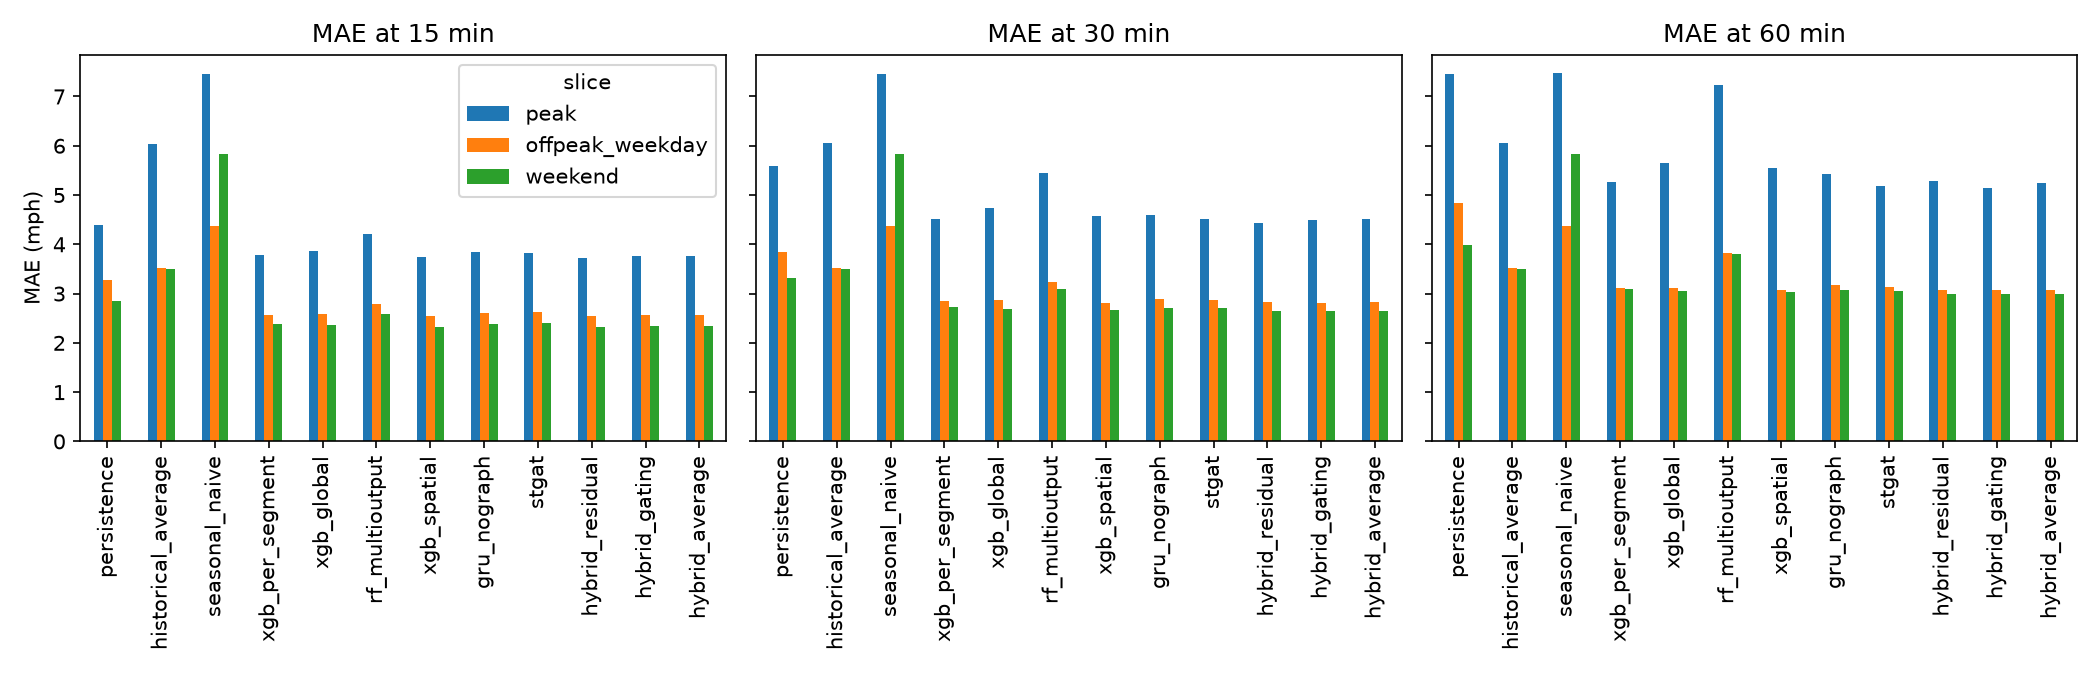
\includegraphics[width=1.00\linewidth]{../../results/figures/peak_offpeak_bars.png}\\[2pt]{\footnotesize\itshape Figure 18. MAE by slice at 15, 30 and 60 minutes.}\end{figure}

\subsection*{12.5 Uncertainty: day-block bootstrap}\addcontentsline{toc}{subsection}{12.5 Uncertainty: day-block bootstrap}
{\scriptsize\renewcommand{\arraystretch}{1.15}\begin{longtable}{>{\raggedright\arraybackslash}p{0.3400\dimexpr\linewidth-8\tabcolsep\relax}>{\raggedright\arraybackslash}p{0.2200\dimexpr\linewidth-8\tabcolsep\relax}>{\raggedright\arraybackslash}p{0.2200\dimexpr\linewidth-8\tabcolsep\relax}>{\raggedright\arraybackslash}p{0.2200\dimexpr\linewidth-8\tabcolsep\relax}}
\toprule
\textbf{Model} & \textbf{15 min} & \textbf{30 min} & \textbf{60 min} \\
\midrule
\endhead
\bottomrule
\endlastfoot
Persistence & 3.49 [3.32, 3.66] & 4.20 [3.96, 4.43] & 5.37 [5.00, 5.73] \\
Historical average & 4.19 [3.94, 4.46] & 4.19 [3.94, 4.46] & 4.19 [3.94, 4.46] \\
Seasonal naive & 5.50 [5.10, 5.96] & 5.50 [5.11, 5.96] & 5.50 [5.10, 5.96] \\
XGBoost per-segment & 2.86 [2.71, 3.01] & 3.28 [3.09, 3.46] & 3.68 [3.47, 3.92] \\
XGBoost global (pooled) & 2.88 [2.72, 3.03] & 3.33 [3.13, 3.53] & 3.78 [3.54, 4.02] \\
Random Forest (multi-output) & 3.14 [2.97, 3.30] & 3.80 [3.58, 4.01] & 4.73 [4.45, 5.02] \\
XGBoost spatial & 2.82 [2.67, 2.96] & 3.26 [3.07, 3.45] & 3.73 [3.50, 3.97] \\
GRU no-graph & 2.89 [2.74, 3.04] & 3.30 [3.11, 3.50] & 3.77 [3.53, 4.00] \\
STGAT & 2.89 [2.74, 3.03] & 3.25 [3.07, 3.44] & 3.67 [3.45, 3.90] \\
Hybrid: residual & 2.82 [2.67, 2.96] & 3.22 [3.04, 3.40] & 3.65 [3.43, 3.88] \\
Hybrid: gating & 2.83 [2.68, 2.98] & 3.22 [3.04, 3.41] & 3.61 [3.39, 3.84] \\
Hybrid: average & 2.83 [2.68, 2.98] & 3.23 [3.05, 3.42] & 3.64 [3.42, 3.87] \\
XGBoost global + daily lag & 2.88 [2.72, 3.03] & 3.33 [3.13, 3.53] & 3.78 [3.54, 4.03] \\
\end{longtable}}
{\footnotesize\itshape Table 33. MAE with 95\% day-block bootstrap intervals (first seed). Intervals of different models overlap because day difficulty dominates; paired tests (DM, paired bootstrap) are needed to compare models.}\par\medskip

\subsection*{12.6 Significance (Diebold--Mariano)}\addcontentsline{toc}{subsection}{12.6 Significance (Diebold--Mariano)}
{\scriptsize\renewcommand{\arraystretch}{1.15}\begin{longtable}{>{\raggedright\arraybackslash}p{0.2000\dimexpr\linewidth-14\tabcolsep\relax}>{\raggedright\arraybackslash}p{0.2000\dimexpr\linewidth-14\tabcolsep\relax}>{\raggedright\arraybackslash}p{0.1000\dimexpr\linewidth-14\tabcolsep\relax}>{\raggedright\arraybackslash}p{0.1300\dimexpr\linewidth-14\tabcolsep\relax}>{\raggedright\arraybackslash}p{0.1100\dimexpr\linewidth-14\tabcolsep\relax}>{\raggedright\arraybackslash}p{0.1000\dimexpr\linewidth-14\tabcolsep\relax}>{\raggedright\arraybackslash}p{0.1600\dimexpr\linewidth-14\tabcolsep\relax}}
\toprule
\textbf{Model A} & \textbf{Model B} & \textbf{Horizon} & \textbf{DM statistic} & \textbf{p-value} & \textbf{Seed pairs} & \textbf{Verdict} \\
\midrule
\endhead
\bottomrule
\endlastfoot
XGBoost spatial & XGBoost global (pooled) & 15 min & -14.42 & 0.0000 & 1 & A better \\
XGBoost spatial & XGBoost global (pooled) & 30 min & -11.55 & 0.0000 & 1 & A better \\
XGBoost spatial & XGBoost global (pooled) & 60 min & -6.89 & 0.0000 & 1 & A better \\
XGBoost global (pooled) & XGBoost per-segment & 15 min & +3.79 & 0.0002 & 1 & B better \\
XGBoost global (pooled) & XGBoost per-segment & 30 min & +5.34 & 0.0000 & 1 & B better \\
XGBoost global (pooled) & XGBoost per-segment & 60 min & +6.29 & 0.0000 & 1 & B better \\
XGBoost spatial & XGBoost per-segment & 15 min & -6.31 & 0.0000 & 1 & A better \\
XGBoost spatial & XGBoost per-segment & 30 min & -1.68 & 0.0925 & 1 & no significant difference \\
XGBoost spatial & XGBoost per-segment & 60 min & +2.97 & 0.0030 & 1 & B better \\
XGBoost global (pooled) & Persistence & 15 min & -50.36 & 0.0000 & 1 & A better \\
XGBoost global (pooled) & Persistence & 30 min & -34.82 & 0.0000 & 1 & A better \\
XGBoost global (pooled) & Persistence & 60 min & -22.96 & 0.0000 & 1 & A better \\
STGAT & XGBoost global (pooled) & 15 min & +4.08 & 0.0486 & 3 & B better \\
STGAT & XGBoost global (pooled) & 30 min & -4.69 & 0.0022 & 3 & A better \\
STGAT & XGBoost global (pooled) & 60 min & -5.47 & 0.0000 & 3 & A better \\
STGAT & XGBoost spatial & 15 min & +17.74 & 0.0000 & 3 & B better \\
STGAT & XGBoost spatial & 30 min & +2.42 & 0.6342 & 3 & no significant difference \\
STGAT & XGBoost spatial & 60 min & -3.71 & 0.0095 & 3 & A better \\
STGAT & GRU no-graph & 15 min & +0.43 & 0.7194 & 3 & no significant difference \\
STGAT & GRU no-graph & 30 min & -6.21 & 0.0828 & 3 & no significant difference \\
STGAT & GRU no-graph & 60 min & -6.79 & 0.0000 & 3 & A better \\
STGAT & XGBoost per-segment & 15 min & +6.49 & 0.0000 & 3 & B better \\
STGAT & XGBoost per-segment & 30 min & +0.26 & 0.7975 & 3 & no significant difference \\
STGAT & XGBoost per-segment & 60 min & -0.69 & 0.9771 & 3 & no significant difference \\
Hybrid: residual & XGBoost global (pooled) & 15 min & -12.27 & 0.0000 & 3 & A better \\
Hybrid: residual & XGBoost global (pooled) & 30 min & -10.63 & 0.0000 & 3 & A better \\
Hybrid: residual & XGBoost global (pooled) & 60 min & -9.22 & 0.0000 & 3 & A better \\
Hybrid: residual & STGAT & 15 min & -21.26 & 0.0000 & 3 & A better \\
Hybrid: residual & STGAT & 30 min & -9.44 & 0.0000 & 3 & A better \\
Hybrid: residual & STGAT & 60 min & -1.26 & 0.4802 & 3 & no significant difference \\
Hybrid: residual & Hybrid: average & 15 min & -7.18 & 0.0000 & 3 & A better \\
Hybrid: residual & Hybrid: average & 30 min & -5.22 & 0.0052 & 3 & A better \\
Hybrid: residual & Hybrid: average & 60 min & +1.05 & 0.2915 & 3 & no significant difference \\
Hybrid: gating & XGBoost global (pooled) & 15 min & -12.60 & 0.0000 & 3 & A better \\
Hybrid: gating & XGBoost global (pooled) & 30 min & -10.57 & 0.0000 & 3 & A better \\
Hybrid: gating & XGBoost global (pooled) & 60 min & -9.94 & 0.0000 & 3 & A better \\
Hybrid: gating & STGAT & 15 min & -25.16 & 0.0000 & 3 & A better \\
Hybrid: gating & STGAT & 30 min & -13.03 & 0.0000 & 3 & A better \\
Hybrid: gating & STGAT & 60 min & -11.33 & 0.0000 & 3 & A better \\
Hybrid: average & XGBoost global (pooled) & 15 min & -10.92 & 0.0000 & 3 & A better \\
Hybrid: average & XGBoost global (pooled) & 30 min & -11.81 & 0.0000 & 3 & A better \\
Hybrid: average & XGBoost global (pooled) & 60 min & -10.86 & 0.0000 & 3 & A better \\
Hybrid: average & STGAT & 15 min & -25.50 & 0.0000 & 3 & A better \\
Hybrid: average & STGAT & 30 min & -5.98 & 0.0000 & 3 & A better \\
Hybrid: average & STGAT & 60 min & -3.05 & 0.0131 & 3 & A better \\
\end{longtable}}
{\footnotesize\itshape Table 34. Diebold--Mariano tests (negative statistic: model A has lower loss; p is the largest over seed pairs).}\par\medskip

\clearpage
\section*{13. Ablation studies}\addcontentsline{toc}{section}{13. Ablation studies}
Each ablation changes one setting from the STGAT default. Budget (to suit a laptop): \textbf{one seed and 12 epochs} per run, with a re-run of the default under the same budget as the reference (A0). Runs with different history lengths have different first test windows, so all runs are compared on the 6,820 test anchors they share. Differences of a few hundredths of a mph are within seed noise (the 3-seed std of the full STGAT runs is 0.011--0.022 mph).

{\scriptsize\renewcommand{\arraystretch}{1.15}\begin{longtable}{>{\raggedright\arraybackslash}p{0.0600\dimexpr\linewidth-18\tabcolsep\relax}>{\raggedright\arraybackslash}p{0.3400\dimexpr\linewidth-18\tabcolsep\relax}>{\raggedright\arraybackslash}p{0.0900\dimexpr\linewidth-18\tabcolsep\relax}>{\raggedright\arraybackslash}p{0.0900\dimexpr\linewidth-18\tabcolsep\relax}>{\raggedright\arraybackslash}p{0.0900\dimexpr\linewidth-18\tabcolsep\relax}>{\raggedright\arraybackslash}p{0.0800\dimexpr\linewidth-18\tabcolsep\relax}>{\raggedright\arraybackslash}p{0.0800\dimexpr\linewidth-18\tabcolsep\relax}>{\raggedright\arraybackslash}p{0.0800\dimexpr\linewidth-18\tabcolsep\relax}>{\raggedright\arraybackslash}p{0.0900\dimexpr\linewidth-18\tabcolsep\relax}}
\toprule
\textbf{ID} & \textbf{Change} & \textbf{MAE 15} & \textbf{MAE 30} & \textbf{MAE 60} & \textbf{\ensuremath{\Delta}15} & \textbf{\ensuremath{\Delta}30} & \textbf{\ensuremath{\Delta}60} & \textbf{Time (s)} \\
\midrule
\endhead
\bottomrule
\endlastfoot
A0 & reference (bidirectional graph, GAT, 4 heads, 2 layers) & 2.984 & 3.407 & 3.955 & +0.000 & +0.000 & +0.000 & 509 \\
A1 & no neighbours & 2.954 & 3.372 & 3.820 & -0.030 & -0.035 & -0.135 & 318 \\
A2 & random graph, same edge count & 3.027 & 3.477 & 4.043 & +0.043 & +0.069 & +0.088 & 380 \\
A3 & W\ensuremath{^{\top}} only (upstream senders) & 2.995 & 3.416 & 3.956 & +0.011 & +0.009 & +0.001 & 400 \\
A3 & W only (downstream senders) & 2.998 & 3.421 & 3.942 & +0.014 & +0.014 & -0.013 & 417 \\
A4 & GATv2 attention & 2.953 & 3.376 & 3.934 & -0.031 & -0.031 & -0.021 & 3828 \\
A4 & fixed row-normalised weights & 2.957 & 3.385 & 3.893 & -0.027 & -0.023 & -0.062 & 205 \\
A5 & 1 head & 2.967 & 3.385 & 3.895 & -0.017 & -0.022 & -0.060 & 450 \\
A5 & 2 heads & 2.965 & 3.381 & 3.919 & -0.019 & -0.026 & -0.036 & 474 \\
A5 & 8 heads & 2.974 & 3.403 & 3.946 & -0.010 & -0.004 & -0.009 & 536 \\
A6 & 1 block & 2.992 & 3.437 & 4.024 & +0.008 & +0.030 & +0.069 & 257 \\
A6 & 3 blocks & 2.976 & 3.408 & 3.963 & -0.008 & +0.001 & +0.008 & 728 \\
A7 & no node embedding & 3.132 & 3.728 & 4.581 & +0.149 & +0.321 & +0.626 & 486 \\
A8 & no calendar channels & 3.077 & 3.685 & 4.643 & +0.093 & +0.278 & +0.688 & 490 \\
A9 & zeros kept + mask (DCRNN style) & 3.002 & 3.425 & 3.964 & +0.018 & +0.017 & +0.009 & 493 \\
A10 & dropout 0 & 2.947 & 3.371 & 3.866 & -0.037 & -0.036 & -0.089 & 485 \\
A10 & weight decay 0 & 2.929 & 3.310 & 3.731 & -0.055 & -0.097 & -0.224 & 493 \\
A11 & history 24 steps & 2.978 & 3.396 & 3.895 & -0.006 & -0.011 & -0.060 & 576 \\
A11 & history 6 steps & 2.975 & 3.397 & 3.934 & -0.009 & -0.010 & -0.021 & 453 \\
A12 & distance bias in attention & 2.951 & 3.372 & 3.899 & -0.033 & -0.035 & -0.056 & 497 \\
\end{longtable}}
{\footnotesize\itshape Table 35. Ablation results (\ensuremath{\Delta} vs A0; negative = better than the default).}\par\medskip

\begin{itemize}[nosep,leftmargin=*]
\item \textbf{No graph benefit shown under this budget:} the identity graph (A1) is not worse than the road graph --- at 60 minutes it is better.
\item \textbf{Wrong edges hurt:} a random graph with the same number of edges (A2) is worse than both, weak evidence that topology matters.
\item \textbf{What matters most:} removing the node embedding (A7) or the calendar features (A8) costs 0.6--0.7 mph at 60 minutes.
\item \textbf{Within noise:} edge direction (A3), attention type (A4), heads (A5), depth (A6), imputation (A9), history length (A11), edge bias (A12).
\item \textbf{Regularisation (A10):} removing dropout or weight decay helped --- with only 12 epochs the model is under-trained, so this says nothing about full training.
\item \textbf{A13 (hybrid design):} residual vs gating vs average, read from the main table (Section 11).
\item The 3-seed, 40-epoch comparison with the GRU (Section 10.7) remains the stronger evidence that the graph helps at 60 minutes.
\end{itemize}

\begin{figure}[H]\centering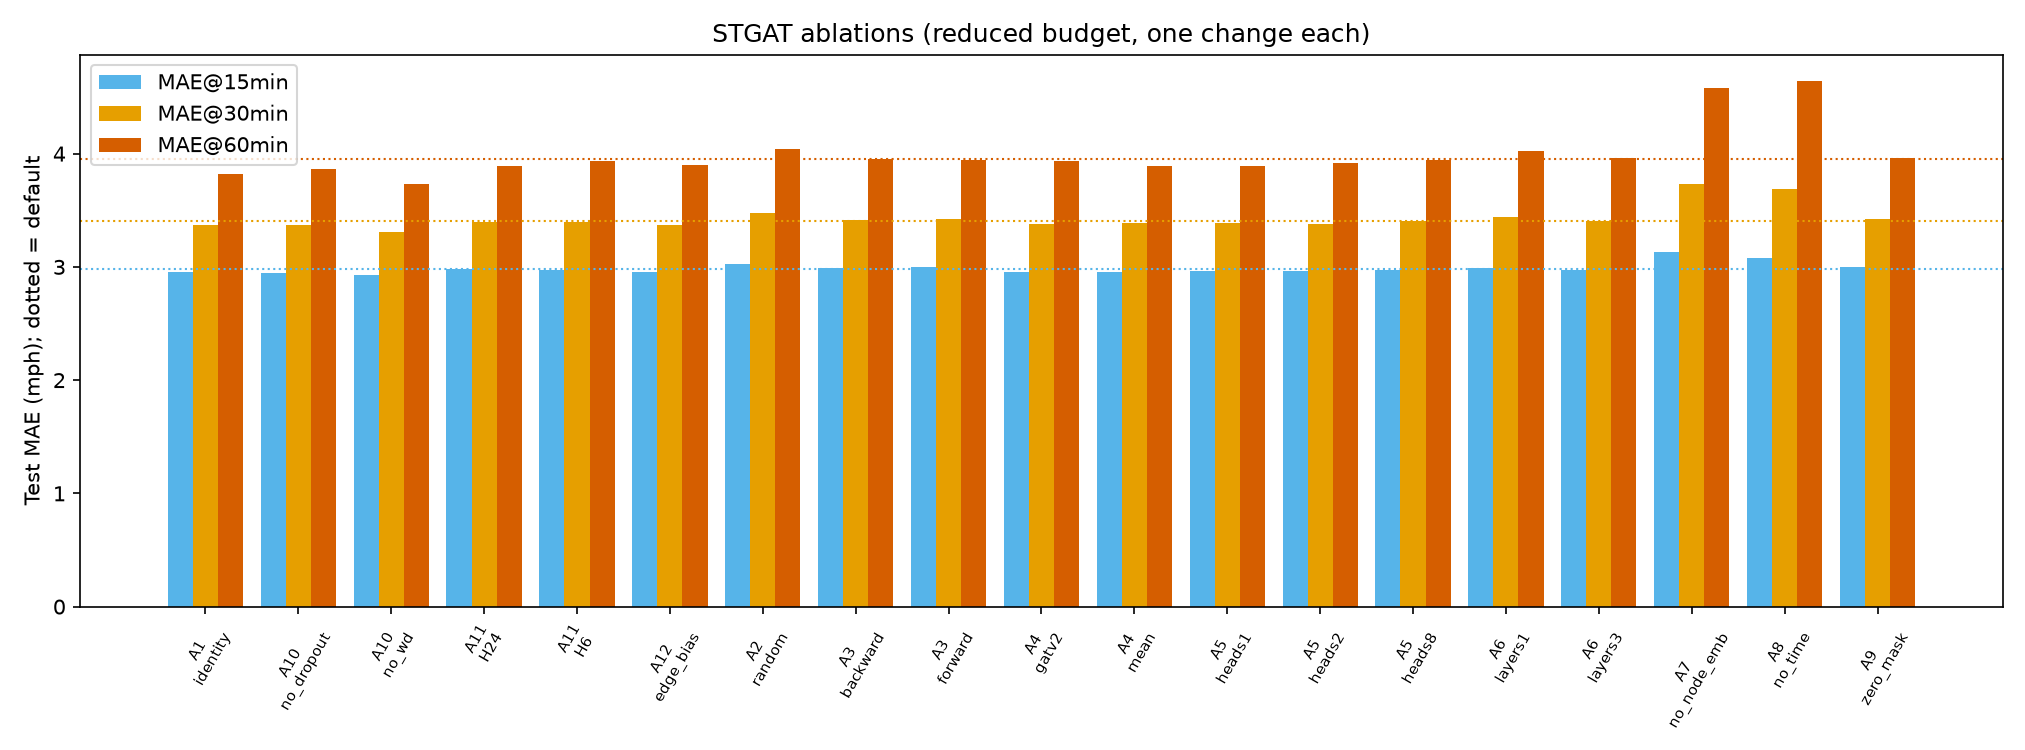
\includegraphics[width=1.00\linewidth]{../../results/figures/ablations/ablation_bars.png}\\[2pt]{\footnotesize\itshape Figure 19. Ablation MAE at 15/\allowbreak{}30/\allowbreak{}60 minutes (dotted lines: default).}\end{figure}

\clearpage
\section*{14. Maps and interpretability}\addcontentsline{toc}{section}{14. Maps and interpretability}
\subsection*{14.1 Forecast maps}\addcontentsline{toc}{subsection}{14.1 Forecast maps}
The AM-peak map anchor is chosen automatically: the test weekday window whose 15-minute targets fall in 07:00--09:00 with the most congested observed sensors --- anchor index 608 with targets 2012-06-06 08:35:00 (+15 min), 2012-06-06 08:50:00 (+30) and 2012-06-06 09:20:00 (+60). Interactive files: \texttt{results/\allowbreak{}maps/\allowbreak{}forecast\_\allowbreak{}am\_\allowbreak{}peak.html} (truth, STGAT, XGB-global at three horizons, toggleable layers) and \texttt{animated\_\allowbreak{}peak\_\allowbreak{}truth.html} /\allowbreak{} \texttt{animated\_\allowbreak{}peak\_\allowbreak{}stgat.html} (time slider over one peak hour). Colours: red < 40 mph, orange 40--55, green > 55, grey missing.

\subsection*{14.2 Where the graph model helps}\addcontentsline{toc}{subsection}{14.2 Where the graph model helps}
\begin{figure}[H]\centering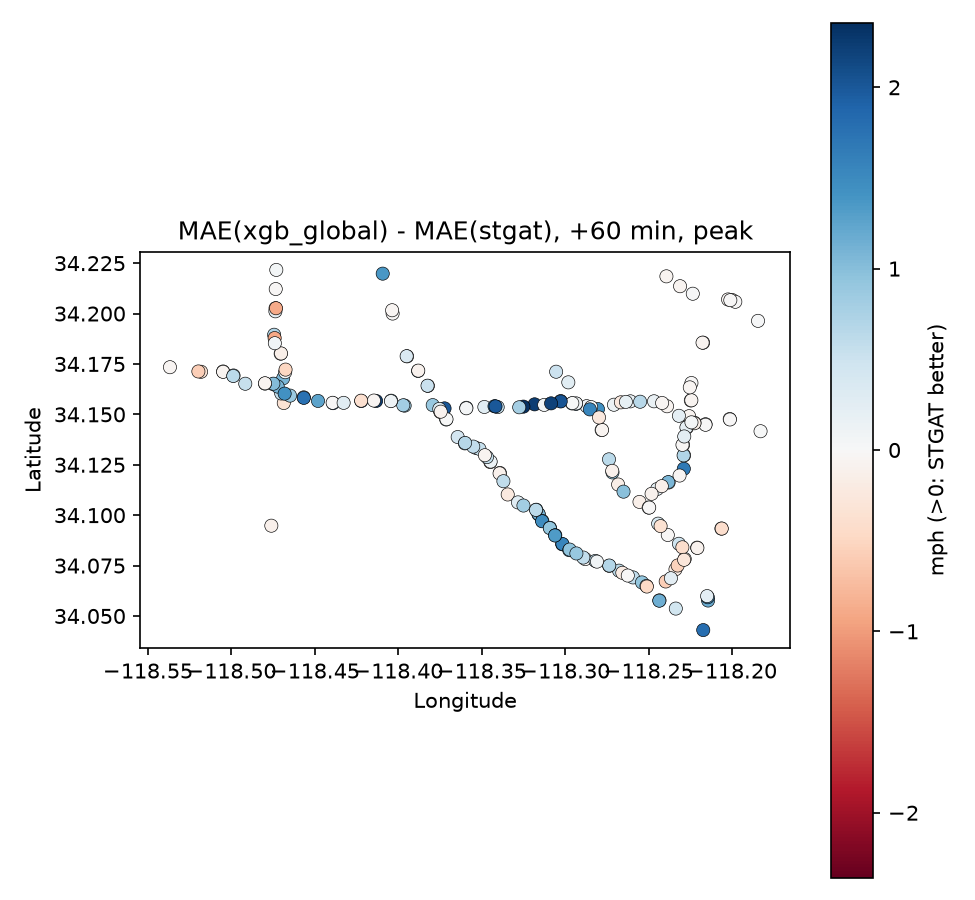
\includegraphics[width=0.76\linewidth]{../../results/figures/maps/error_diff_h12_peak.png}\\[2pt]{\footnotesize\itshape Figure 20. Per-sensor MAE(XGB-global) \ensuremath{-} MAE(STGAT) at 60 minutes during peaks (blue: STGAT better).}\end{figure}

Gains cluster along specific freeway segments; a few sensors are slightly worse with STGAT.

\subsection*{14.3 Space-time diagram}\addcontentsline{toc}{subsection}{14.3 Space-time diagram}
A corridor of 18 sensors is found automatically by following the nearest downstream neighbour with increasing road distance from each start sensor and keeping the longest chain. The day shown (2012-06-21) is the test weekday with the most corridor congestion between 05:00 and 11:00. Neither model anticipates the abrupt breakdown near 10:00 --- onset is the hardest event to forecast.

\begin{figure}[H]\centering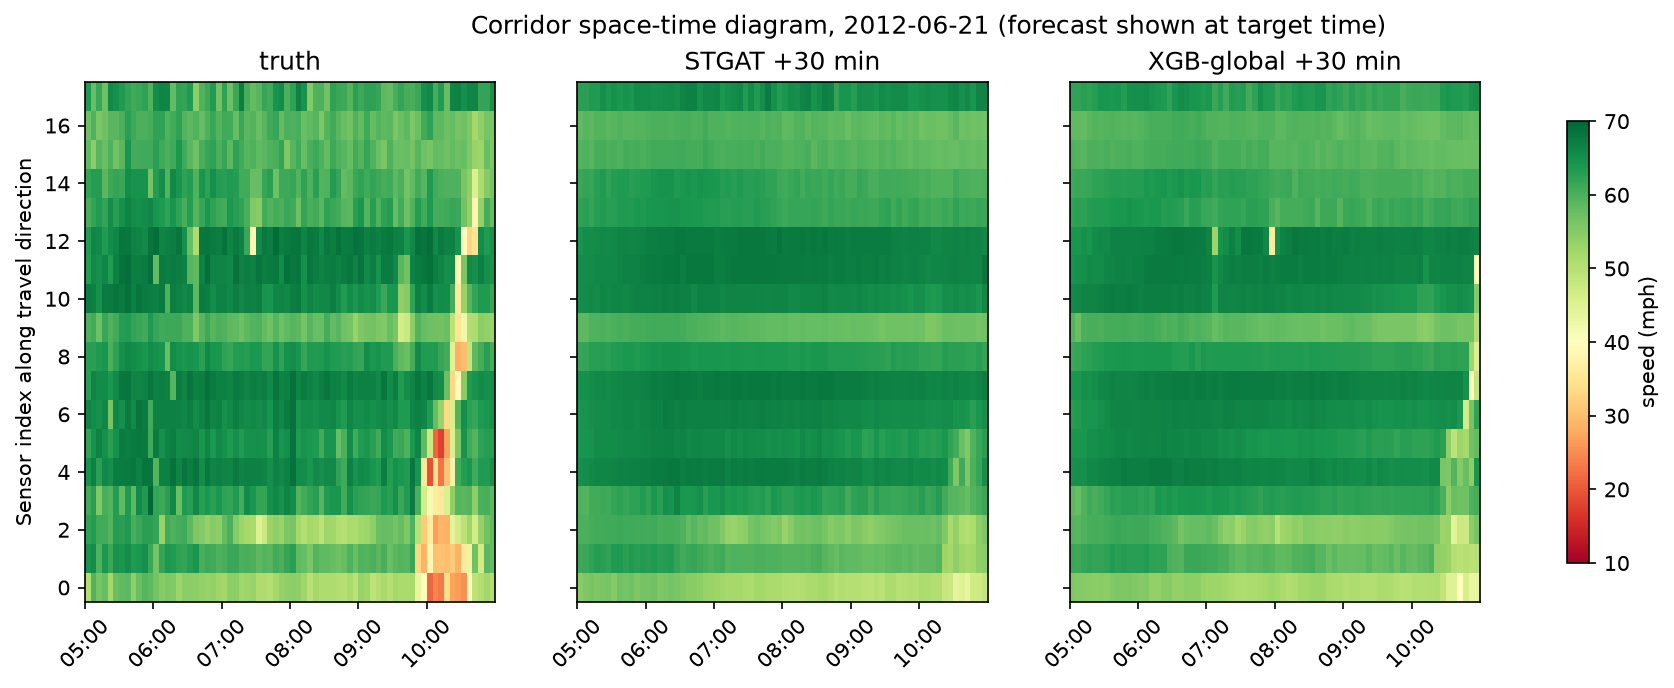
\includegraphics[width=1.00\linewidth]{../../results/figures/maps/space_time.png}\\[2pt]{\footnotesize\itshape Figure 21. Corridor space-time diagram: truth, STGAT and XGB-global 30-minute forecasts placed at their target time.}\end{figure}

\subsection*{14.4 Attention (qualitative)}\addcontentsline{toc}{subsection}{14.4 Attention (qualitative)}
{\scriptsize\renewcommand{\arraystretch}{1.15}\begin{longtable}{>{\raggedright\arraybackslash}p{0.1600\dimexpr\linewidth-12\tabcolsep\relax}>{\raggedright\arraybackslash}p{0.1800\dimexpr\linewidth-12\tabcolsep\relax}>{\raggedright\arraybackslash}p{0.1400\dimexpr\linewidth-12\tabcolsep\relax}>{\raggedright\arraybackslash}p{0.1800\dimexpr\linewidth-12\tabcolsep\relax}>{\raggedright\arraybackslash}p{0.1700\dimexpr\linewidth-12\tabcolsep\relax}>{\raggedright\arraybackslash}p{0.1700\dimexpr\linewidth-12\tabcolsep\relax}}
\toprule
\textbf{Period} & \textbf{Windows averaged} & \textbf{Self} & \textbf{Downstream only} & \textbf{Upstream only} & \textbf{Both directions} \\
\midrule
\endhead
\bottomrule
\endlastfoot
am peak & 72 & 10.1\% & 39.3\% & 39.0\% & 11.6\% \\
night & 136 & 9.9\% & 39.0\% & 39.2\% & 12.0\% \\
\end{longtable}}
{\footnotesize\itshape Table 36. Share of last-block attention mass (STGAT seed 0, heads averaged), test weekdays: AM peak = anchors 07:30--08:30, night = 02:00--04:00.}\par\medskip

The shares are the same at the AM peak and at night, so we find no peak-specific shift of attention towards upstream or downstream sensors. Attention is a probe, not causal evidence.

\begin{figure}[H]\centering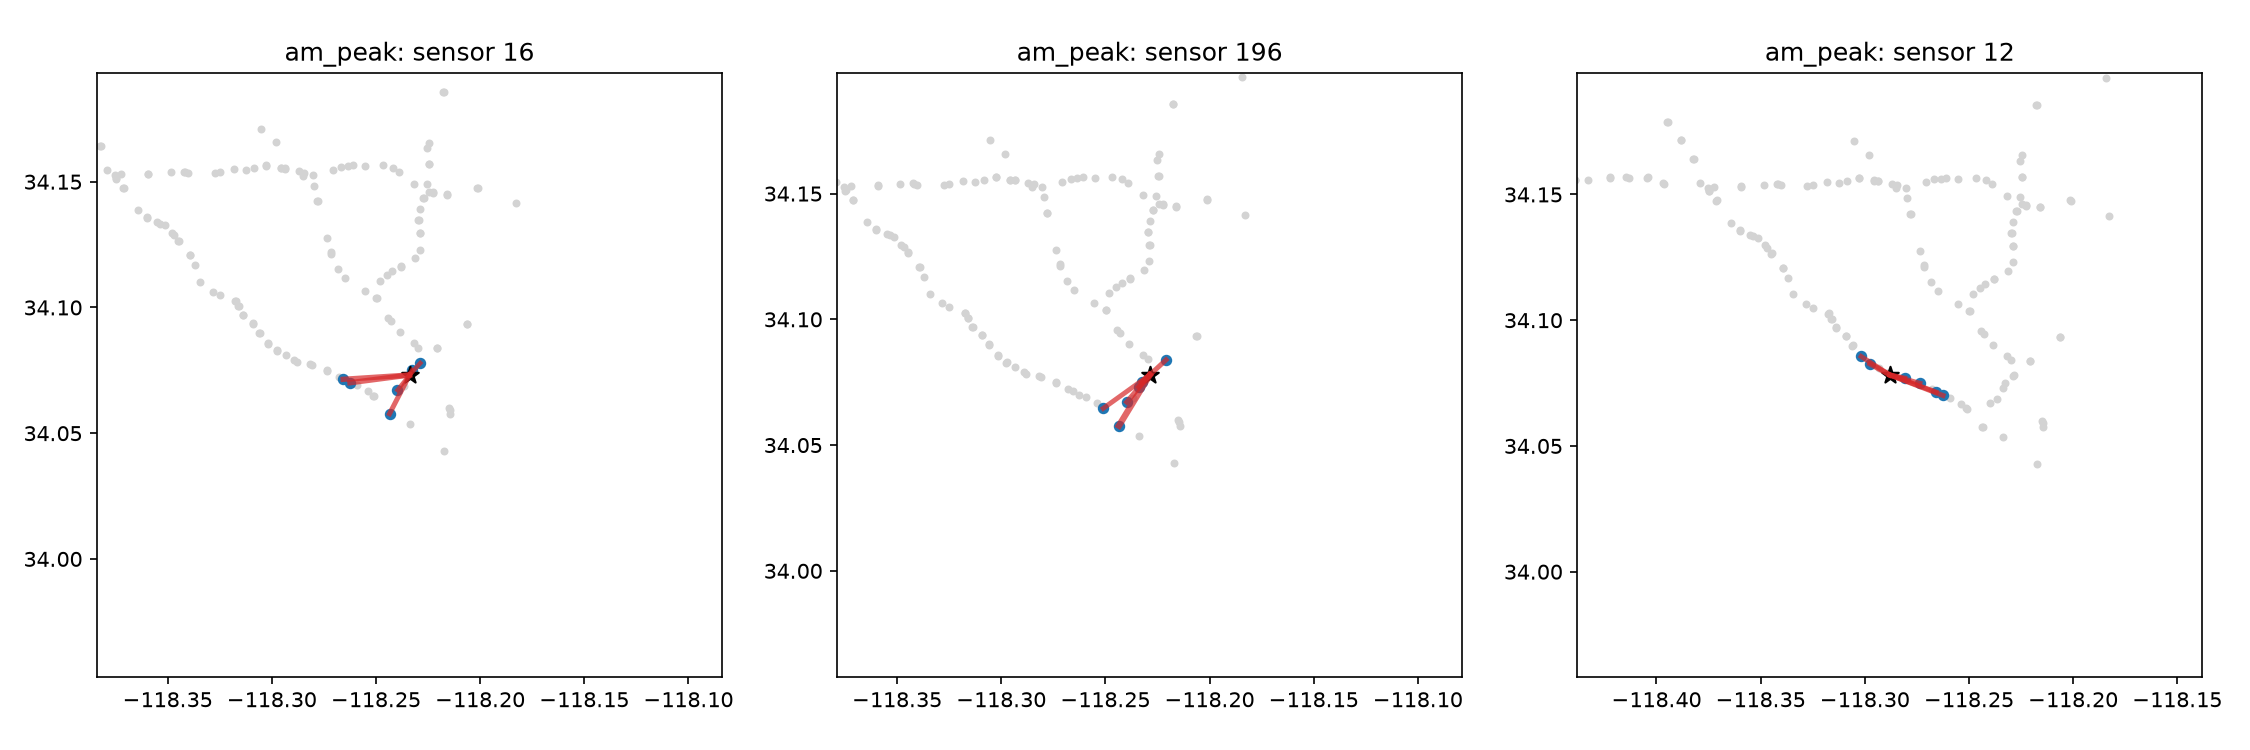
\includegraphics[width=1.00\linewidth]{../../results/figures/maps/attention_am_peak.png}\\[2pt]{\footnotesize\itshape Figure 22. Strongest attention links for the three most congested sensors, AM peak.}\end{figure}

\clearpage
\section*{15. Simulated ramp-metering experiment}\addcontentsline{toc}{section}{15. Simulated ramp-metering experiment}
\begin{callout}This is an offline simulation on a synthetic network. It demonstrates how forecasts could inform a control policy. No live or real-world traffic control is performed or claimed.\end{callout}

\subsection*{15.1 Why ramp metering}\addcontentsline{toc}{subsection}{15.1 Why ramp metering}
METR-LA sensors are on freeways, which have no traffic signals; the realistic control analogue is on-ramp metering.

\subsection*{15.2 Cell Transmission Model}\addcontentsline{toc}{subsection}{15.2 Cell Transmission Model}
{\scriptsize\renewcommand{\arraystretch}{1.15}\begin{longtable}{>{\raggedright\arraybackslash}p{0.2400\dimexpr\linewidth-4\tabcolsep\relax}>{\raggedright\arraybackslash}p{0.7600\dimexpr\linewidth-4\tabcolsep\relax}}
\toprule
\textbf{Element} & \textbf{Setting} \\
\midrule
\endhead
\bottomrule
\endlastfoot
Corridor & 12 cells \ensuremath{\times} 0.5 mile, 3 lanes, time step 10 s (CFL: 65 mph \ensuremath{\times} 10 s = 0.18 mi \ensuremath{\leq} 0.5 mi) \\
Fundamental diagram & triangular: free-flow 65 mph, capacity 2,000 veh/\allowbreak{}h/\allowbreak{}lane, jam density 200 veh/\allowbreak{}mi/\allowbreak{}lane, critical density 30.8, backward wave \ensuremath{\approx} 11.8 mph \\
On-ramps & cells 2, 5, 8; maximum ramp discharge 1,800 veh/\allowbreak{}h \\
Bottleneck & cell 10 at 75\% capacity (lane-drop-like) \\
Capacity drop & congested cells (lane density > 1.15 \ensuremath{\times} critical) discharge at 88\% of capacity \\
Merge rule & mainline gets 70\% priority when the receiving cell cannot take both flows \\
Upstream boundary & virtual queue for demand that cannot enter \\
\end{longtable}}
{\footnotesize\itshape Table 37. Simulator settings (\texttt{src/\allowbreak{}traffic/\allowbreak{}control/\allowbreak{}ctm.py}).}\par\medskip

Tests check vehicle conservation (in \ensuremath{-} out \ensuremath{-} stored = 0 to 1e-6), free flow at low demand, a queue that grows upstream of the bottleneck, ALINEA direction and clipping, and the speed-to-occupancy conversion.

\subsection*{15.3 Demand (synthetic, shaped by METR-LA)}\addcontentsline{toc}{subsection}{15.3 Demand (synthetic, shaped by METR-LA)}
METR-LA has no flow, and speed cannot be inverted to flow in free flow (all sub-critical densities share one speed). Demand is therefore synthetic, shaped by a congestion index computed from the 12 corridor sensors mapped to the cells:

\begin{eqbox}ci(t) = clip( ((65 \ensuremath{-} mean speed(t)) /\allowbreak{} 45) /\allowbreak{} ci\_\allowbreak{}ref , 0, 1 ),   ci\_\allowbreak{}ref = 0.167 (95th percentile, training weekdays 05:00--11:00)\end{eqbox}

\begin{eqbox}mainline demand = 6000 \ensuremath{\cdot} (0.45 + 0.22 \ensuremath{\cdot} ci) veh/\allowbreak{}h        each ramp = 250 + 150 \ensuremath{\cdot} ci veh/\allowbreak{}h\end{eqbox}

At ci = 1 total demand is about 16\% above the bottleneck capacity. Simulated 04:30--11:00, scored 05:00--11:00, on the five test weekdays with the most AM corridor congestion: 2012-06-21, 2012-06-12, 2012-06-15, 2012-06-07, 2012-06-26.

\subsection*{15.4 Policies}\addcontentsline{toc}{subsection}{15.4 Policies}
\begin{itemize}[nosep,leftmargin=*]
\item \textbf{No control:} ramps unmetered.
\item \textbf{Fixed-time:} one rate 06:00--10:00, tuned on the validation weekday 2012-05-29 over the grid [200, 250, 300, 350, 400, 500] veh/\allowbreak{}h; rates \ensuremath{\geq} 350 tied (TTS 4788.8 veh\ensuremath{\cdot}h, identical to no control), and 400 was selected --- non-binding, so it equals no control.
\item \textbf{ALINEA:} r(k) = r(k \ensuremath{-} 1) + 70 \ensuremath{\cdot} (o* \ensuremath{-} o(k)) every 60 s, o = occupancy (\%) of the cell downstream of the ramp, o* = critical occupancy 15.4\%, rates clipped to 200--1,800 veh/\allowbreak{}h.
\item \textbf{Predictive ALINEA (literal spec):} occupancy = max(measured, occupancy implied by the STGAT +15-minute speed forecast via the congested branch \ensuremath{\rho} = w\ensuremath{\cdot}\ensuremath{\rho}\_\allowbreak{}jam/\allowbreak{}(v + w)).
\item \textbf{Look-ahead ALINEA:} a copy of the simulator is rolled 15 minutes ahead from its live state with demand moving to the forecast congestion index; ALINEA uses max(measured, look-ahead occupancy).
\item \textbf{Oracle versions} of both use the true future speeds (upper bound).
\end{itemize}

\subsection*{15.5 Results}\addcontentsline{toc}{subsection}{15.5 Results}
{\scriptsize\renewcommand{\arraystretch}{1.15}\begin{longtable}{>{\raggedright\arraybackslash}p{0.2000\dimexpr\linewidth-12\tabcolsep\relax}>{\raggedright\arraybackslash}p{0.1600\dimexpr\linewidth-12\tabcolsep\relax}>{\raggedright\arraybackslash}p{0.1600\dimexpr\linewidth-12\tabcolsep\relax}>{\raggedright\arraybackslash}p{0.1600\dimexpr\linewidth-12\tabcolsep\relax}>{\raggedright\arraybackslash}p{0.1600\dimexpr\linewidth-12\tabcolsep\relax}>{\raggedright\arraybackslash}p{0.1600\dimexpr\linewidth-12\tabcolsep\relax}}
\toprule
\textbf{Policy} & \textbf{TTS (veh\ensuremath{\cdot}h)} & \textbf{Mainline speed (mph)} & \textbf{Max ramp queue (veh)} & \textbf{Congested cell-minutes} & \textbf{Distance (veh\ensuremath{\cdot}mi)} \\
\midrule
\endhead
\bottomrule
\endlastfoot
no control & 2,704.8 \ensuremath{\pm} 426.4 & 52.4 \ensuremath{\pm} 7.5 & 0.0 \ensuremath{\pm} 0.0 & 399.2 \ensuremath{\pm} 275.4 & 139,350.3 \ensuremath{\pm} 3,088.3 \\
fixed time & 2,704.8 \ensuremath{\pm} 426.4 & 52.4 \ensuremath{\pm} 7.5 & 0.0 \ensuremath{\pm} 0.0 & 399.2 \ensuremath{\pm} 275.4 & 139,350.3 \ensuremath{\pm} 3,088.3 \\
alinea & 2,705.5 \ensuremath{\pm} 426.6 & 57.1 \ensuremath{\pm} 4.4 & 221.3 \ensuremath{\pm} 111.0 & 243.3 \ensuremath{\pm} 148.5 & 139,644.5 \ensuremath{\pm} 3,230.8 \\
predictive alinea & 4,783.5 \ensuremath{\pm} 464.0 & 62.0 \ensuremath{\pm} 1.5 & 766.0 \ensuremath{\pm} 55.3 & 78.6 \ensuremath{\pm} 43.2 & 137,226.1 \ensuremath{\pm} 3,011.2 \\
oracle predictive alinea & 3,854.6 \ensuremath{\pm} 363.1 & 61.3 \ensuremath{\pm} 1.9 & 607.0 \ensuremath{\pm} 61.5 & 97.9 \ensuremath{\pm} 62.0 & 137,879.5 \ensuremath{\pm} 3,170.9 \\
lookahead alinea & 2,714.7 \ensuremath{\pm} 434.2 & 58.2 \ensuremath{\pm} 4.2 & 243.9 \ensuremath{\pm} 117.4 & 201.8 \ensuremath{\pm} 142.5 & 139,656.5 \ensuremath{\pm} 3,221.4 \\
oracle lookahead alinea & 2,728.3 \ensuremath{\pm} 435.6 & 58.1 \ensuremath{\pm} 3.8 & 248.4 \ensuremath{\pm} 117.0 & 204.2 \ensuremath{\pm} 128.6 & 139,647.8 \ensuremath{\pm} 3,240.2 \\
\end{longtable}}
{\footnotesize\itshape Table 38. Simulation results, mean \ensuremath{\pm} std over the five test weekdays.}\par\medskip

\begin{itemize}[nosep,leftmargin=*]
\item ALINEA cuts congested cell-minutes from \ensuremath{\approx} 399 to \ensuremath{\approx} 243 and raises mainline speed from \ensuremath{\approx} 52 to \ensuremath{\approx} 57 mph, but total time spent is unchanged: the delay moves to the ramps.
\item Look-ahead ALINEA behaves like ALINEA; its oracle version is no better, so better forecasts would not help this controller here.
\item The literal forecast-speed variant over-meters (very long ramp queues, much higher TTS) because real-data forecasts do not respond to the simulator's own state (open loop).
\item Conclusion: in this simulation, forecasts gave no measurable benefit.
\end{itemize}

\begin{figure}[H]\centering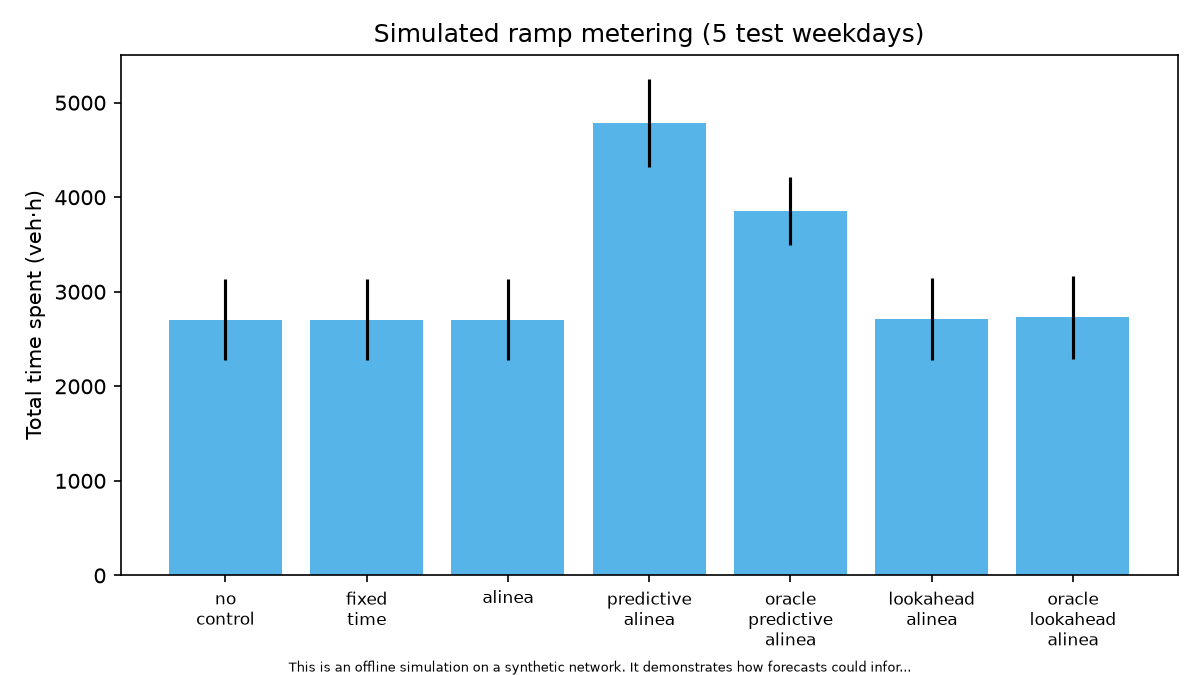
\includegraphics[width=0.79\linewidth]{../../results/figures/control/tts_by_policy.png}\\[2pt]{\footnotesize\itshape Figure 23. Total time spent by policy (offline simulation).}\end{figure}

\begin{figure}[H]\centering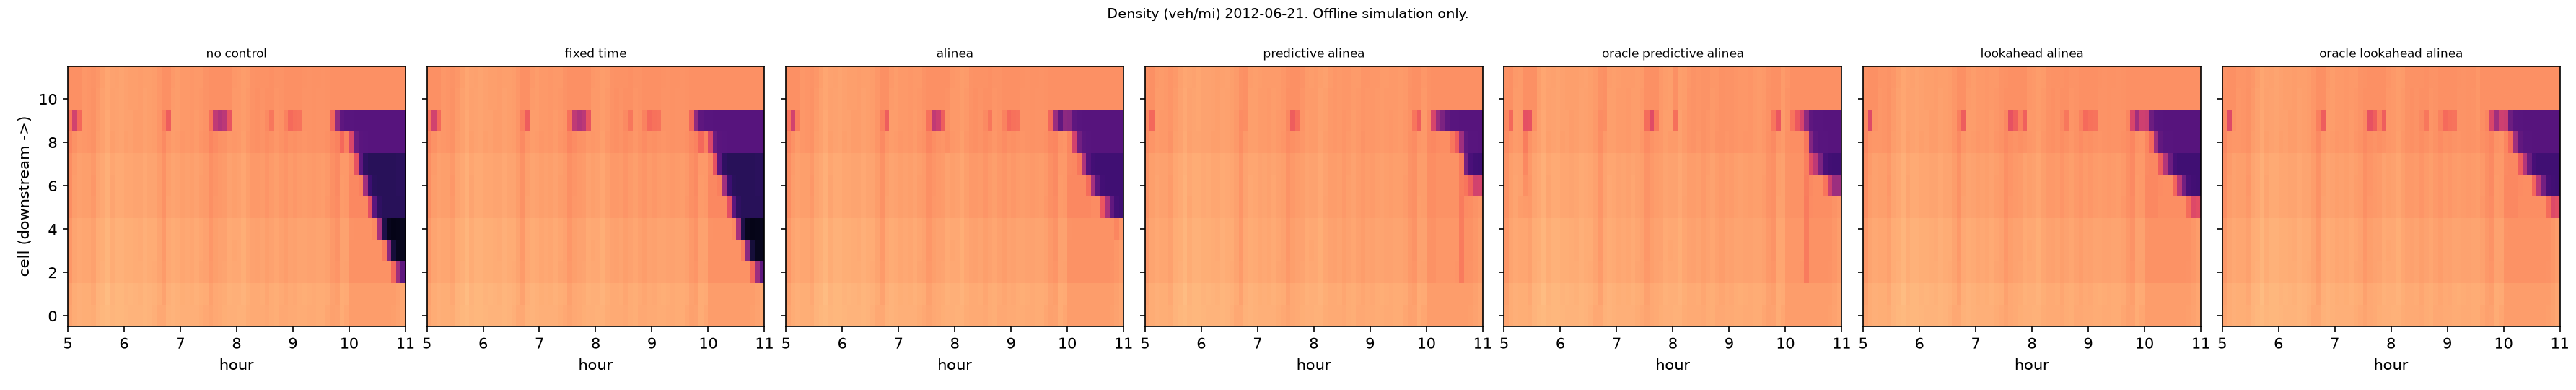
\includegraphics[width=1.00\linewidth]{../../results/figures/control/density_heatmaps.png}\\[2pt]{\footnotesize\itshape Figure 24. Simulated density (veh/\allowbreak{}mi) along the corridor per policy, one test day (offline simulation).}\end{figure}

\clearpage
\section*{16. Engineering and reproducibility}\addcontentsline{toc}{section}{16. Engineering and reproducibility}
\subsection*{16.1 Repository layout}\addcontentsline{toc}{subsection}{16.1 Repository layout}
{\scriptsize\renewcommand{\arraystretch}{1.15}\begin{longtable}{>{\raggedright\arraybackslash}p{0.2800\dimexpr\linewidth-4\tabcolsep\relax}>{\raggedright\arraybackslash}p{0.7200\dimexpr\linewidth-4\tabcolsep\relax}}
\toprule
\textbf{Path} & \textbf{Content} \\
\midrule
\endhead
\bottomrule
\endlastfoot
src/\allowbreak{}traffic/\allowbreak{}data & loading, graph, missing data, split, scaling, windows, datasets, pipeline \\
src/\allowbreak{}traffic/\allowbreak{}features & calendar, lag, neighbour features; tabular design matrices \\
src/\allowbreak{}traffic/\allowbreak{}models & baselines, ML models, GAT layers, STGAT, GRU, hybrid, factory \\
src/\allowbreak{}traffic/\allowbreak{}training & masked losses, trainer, Optuna tuning \\
src/\allowbreak{}traffic/\allowbreak{}evaluation & prediction format, metrics, slices, significance, tables, report numbers \\
src/\allowbreak{}traffic/\allowbreak{}viz & EDA plots, maps, horizon plots, attention plots \\
src/\allowbreak{}traffic/\allowbreak{}control & CTM, ALINEA, predictive ALINEA, experiment \\
scripts/\allowbreak{} & entry points (download, EDA, train\_\allowbreak{}ml, train\_\allowbreak{}dl, make\_\allowbreak{}oof, train\_\allowbreak{}hybrid, ablations, evaluate, maps, control, report assets) and chain scripts \\
configs/\allowbreak{} & base.yaml, ml/\allowbreak{}\emph{, dl/\allowbreak{}}, hybrid/\allowbreak{}\emph{; tuned parameters in ml/\allowbreak{}}.best.yaml \\
tests/\allowbreak{} & unit and end-to-end tests \\
results/\allowbreak{}metrics & all CSV/\allowbreak{}JSON results (tracked) \\
results/\allowbreak{}figures, results/\allowbreak{}maps & figures (tracked) and interactive HTML maps \\
report/\allowbreak{}phase1, report/\allowbreak{}phase2 & IEEE reports; every number comes from generated macros in report/\allowbreak{}tables/\allowbreak{}numbers.tex \\
docs/\allowbreak{} & EDA summary, analyses, theory notes (11), viva preparation, decisions (ADRs), workflow \\
\end{longtable}}
{\footnotesize\itshape Table 39. Repository structure.}\par\medskip

\subsection*{16.2 Tests}\addcontentsline{toc}{subsection}{16.2 Tests}
61 tests pass (pytest), and \texttt{ruff} and \texttt{black} report a clean code base. Key tests: integrity of the raw data; graph rebuild equals the pickle; direction convention on a hand-built chain; no window crosses a split; scaler and imputation statistics depend on training data only; window alignment; features never use the future; tabular row order; masked metrics against hand-computed values; DM and bootstrap behaviour; GAT equals PyG (GATConv, GATv2Conv) and sparse equals dense; the temporal convolution is causal; an identity graph isolates nodes; the hybrid starts exactly at the base forecast; OOF folds never overlap; CTM conserves vehicles; every model runs end to end in debug mode.

\subsection*{16.3 Decision records}\addcontentsline{toc}{subsection}{16.3 Decision records}
{\scriptsize\renewcommand{\arraystretch}{1.15}\begin{longtable}{>{\raggedright\arraybackslash}p{0.1000\dimexpr\linewidth-4\tabcolsep\relax}>{\raggedright\arraybackslash}p{0.9000\dimexpr\linewidth-4\tabcolsep\relax}}
\toprule
\textbf{ADR} & \textbf{Decision} \\
\midrule
\endhead
\bottomrule
\endlastfoot
001 & Standalone git repository for the project folder \\
002 & Graph direction convention: row i aggregates from column j \\
003 & Missing inputs set to the training mean in scaled space plus an is\_\allowbreak{}missing channel \\
004 & PyTables fallback for reading metr-la.h5 \\
005 & Metric, slice, DM-test and bootstrap conventions \\
006 & Reduced ML budget for a laptop \\
007 & Cheaper STGAT training (spatial steps, epoch fraction) \\
008 & Gating hybrid uses part of validation \\
009 & Spec corrections (CityFlow authors; default bidirectional graph) \\
\end{longtable}}
{\footnotesize\itshape Table 40. Architecture decision records (docs/\allowbreak{}decisions.md).}\par\medskip

\subsection*{16.4 Hardware, runtimes and resource limits}\addcontentsline{toc}{subsection}{16.4 Hardware, runtimes and resource limits}
\begin{itemize}[nosep,leftmargin=*]
\item Apple M3 Pro (11 CPU cores, 18 GB RAM); deep models on the integrated GPU through PyTorch MPS.
\item Jobs ran one at a time at low priority (nice), with 6 CPU workers for ML and 4 torch threads, to keep the laptop usable.
\item Approximate wall-clock: ML tuning + training \ensuremath{\approx} 50 min; GRU \ensuremath{\approx} 8 min per seed; STGAT \ensuremath{\approx} 28 min per seed; OOF + residual hybrids \ensuremath{\approx} 80 min; ablations \ensuremath{\approx} 4 h 15 min in total (GATv2 alone \ensuremath{\approx} 64 min).
\end{itemize}

\subsection*{16.5 How to reproduce}\addcontentsline{toc}{subsection}{16.5 How to reproduce}
\begin{itemize}[nosep,leftmargin=*]
\item Create the environment: \texttt{uv venv --python 3.11 .venv}, activate it, \texttt{uv pip install -e ".[dev]"}.
\item \texttt{make data} (download + checks), \texttt{make eda}, \texttt{make phase1} (baselines and tables).
\item \texttt{bash scripts/\allowbreak{}run\_\allowbreak{}ml\_\allowbreak{}chain.sh} (tune and train the four ML models), \texttt{bash scripts/\allowbreak{}run\_\allowbreak{}dl\_\allowbreak{}chain.sh} (GRU and STGAT, 3 seeds).
\item \texttt{bash scripts/\allowbreak{}run\_\allowbreak{}phase2\_\allowbreak{}chain.sh} (OOF base forecasts, hybrids, evaluation, maps, control, report assets).
\item \texttt{bash scripts/\allowbreak{}run\_\allowbreak{}ablation\_\allowbreak{}chain.sh}, then \texttt{python scripts/\allowbreak{}evaluate\_\allowbreak{}ablations.py}.
\item \texttt{make report} builds both PDFs (tectonic). Team members joining the repository run \texttt{python3 join.py} once.
\end{itemize}

\begin{callout}Reproducibility note. Large intermediate files are not tracked by git. During a clean-up of the repository history, three of them were also removed from the working copy: validation-set predictions (results/\allowbreak{}predictions\_\allowbreak{}val), the out-of-fold base forecasts (results/\allowbreak{}hybrid/\allowbreak{}xgb\_\allowbreak{}base.npz) and the per-run ablation predictions (results/\allowbreak{}ablations/\allowbreak{}predictions). All metrics derived from them (main tables, gains, gate weights, ablation table) were already saved and are intact; to re-run the gating hybrid or re-evaluate ablations, regenerate them with the chain scripts above.\end{callout}

\clearpage
\section*{17. Limitations and honest findings}\addcontentsline{toc}{section}{17. Limitations and honest findings}
\subsection*{17.1 Limitations}\addcontentsline{toc}{subsection}{17.1 Limitations}
\begin{itemize}[nosep,leftmargin=*]
\item One city and one season (March--June 2012); speed only (no flow, no occupancy).
\item A fixed distance-based graph that may miss true connectivity (no adaptive adjacency).
\item Reduced budgets: 15 Optuna trials, pooled XGBoost on 25\% of rows with a 400-tree cap that was always reached, the forest on 10\% of rows.
\item STGAT simplified for compute (attention on the last 4 steps, a third of windows per epoch, 40 epochs while still improving).
\item Ablations on one seed and 12 epochs.
\item Literature-protocol (DCRNN) numbers were not produced; only the strict protocol is reported, so results are not directly comparable to published tables.
\item The test period has a higher outage rate than training; MAPE is unstable at low speeds.
\item The control study is synthetic, open loop, and has no ramp-queue override or spill-back modelling.
\item DCRNN-lite and the SUMO intersection alternative were not built (optional in the specification).
\end{itemize}

\subsection*{17.2 Results that did not match the hypothesis}\addcontentsline{toc}{subsection}{17.2 Results that did not match the hypothesis}
\begin{itemize}[nosep,leftmargin=*]
\item Spatial features help, but not more at longer horizons.
\item STGAT equals the no-graph GRU at 15 minutes and beats it only at 60 minutes.
\item In the reduced-budget ablations the road graph did not beat the identity graph.
\item Attention shares were the same at peak and at night.
\item Forecast-informed ramp metering did not reduce total time spent.
\end{itemize}

\subsection*{17.3 Ethics and authorship}\addcontentsline{toc}{subsection}{17.3 Ethics and authorship}
The data are aggregate loop-detector speeds, so privacy risk is low; the main risk is over-claiming real-world control benefits, which this project avoids. Much of the code and documentation was produced with an AI coding assistant and committed as a baseline; team members should follow the course's rules on AI-assisted work and disclose it.

\section*{18. Team T042 and contributions}\addcontentsline{toc}{section}{18. Team T042 and contributions}
{\scriptsize\renewcommand{\arraystretch}{1.15}\begin{longtable}{>{\raggedright\arraybackslash}p{0.0700\dimexpr\linewidth-8\tabcolsep\relax}>{\raggedright\arraybackslash}p{0.1600\dimexpr\linewidth-8\tabcolsep\relax}>{\raggedright\arraybackslash}p{0.2300\dimexpr\linewidth-8\tabcolsep\relax}>{\raggedright\arraybackslash}p{0.5400\dimexpr\linewidth-8\tabcolsep\relax}}
\toprule
\textbf{Rank} & \textbf{Member} & \textbf{GitHub} & \textbf{Owns} \\
\midrule
\endhead
\bottomrule
\endlastfoot
1 & Pranav Singh & Pranav-Singh-Devloper & Deep-learning core: dense/\allowbreak{}sparse GAT layer, STGAT, GRU no-graph, trainer, DL runs, integration and review \\
2 & Kunal & kunaldevsahu & Phase 1 ML (features, XGBoost, Random Forest, Optuna, SHAP, gap analysis) and the hybrid models \\
3 & Himanshu & HimanshuPal29 & Evaluation and statistics framework, baselines, significance tests, simulated control \\
4 & Kanchan & kanchan97-cp & Data pipeline, graph construction, missing-data handling, EDA, ablation runs \\
5 & Vaibhav & VaibhavSingh50 & Scaffold/\allowbreak{}CI, maps and attention plots, README, slides, report assembly \\
\end{longtable}}
{\footnotesize\itshape Table 41. Work split, ordered by difficulty and technical depth.}\par\medskip

Full module lists, report sections, theory notes and individual viva questions are in \texttt{CONTRIBUTIONS.md} and \texttt{docs/\allowbreak{}viva/\allowbreak{}}. Ownership of every file is recorded in \texttt{OWNERS.yaml}.

\section*{Appendix A. Glossary}\addcontentsline{toc}{section}{Appendix A. Glossary}
{\scriptsize\renewcommand{\arraystretch}{1.15}\begin{longtable}{>{\raggedright\arraybackslash}p{0.2200\dimexpr\linewidth-4\tabcolsep\relax}>{\raggedright\arraybackslash}p{0.7800\dimexpr\linewidth-4\tabcolsep\relax}}
\toprule
\textbf{Term} & \textbf{Meaning} \\
\midrule
\endhead
\bottomrule
\endlastfoot
Anchor & the last input time step of a window \\
Horizon h & how far ahead (h \ensuremath{\times} 5 minutes) \\
Masked metric & a metric computed only over observed (non-zero) targets \\
Strict protocol & chronological split with windows built inside each split \\
OOF & out-of-fold: predictions made by a model that did not train on those rows \\
DM test & Diebold--Mariano test of equal predictive accuracy \\
HAC & heteroskedasticity- and autocorrelation-consistent variance (Newey--West) \\
GAT /\allowbreak{} GATv2 & graph attention network; v2 has dynamic attention \\
STGAT & the project's spatio-temporal GAT \\
TTS & total time spent by all vehicles (veh\ensuremath{\cdot}h) \\
CTM & Cell Transmission Model (Daganzo 1994) \\
ALINEA & feedback ramp-metering law (Papageorgiou et al. 1991) \\
MPS & Apple's Metal Performance Shaders backend for PyTorch \\
\end{longtable}}
{\footnotesize\itshape Table 42. Glossary.}\par\medskip

\section*{Appendix B. References}\addcontentsline{toc}{section}{Appendix B. References}
\begin{enumerate}[nosep,leftmargin=*]
\item Veličković et al., Graph Attention Networks, ICLR 2018.
\item Brody, Alon, Yahav, How Attentive are Graph Attention Networks?, ICLR 2022.
\item Kipf and Welling, Semi-Supervised Classification with Graph Convolutional Networks, ICLR 2017.
\item Li, Yu, Shahabi, Liu, Diffusion Convolutional Recurrent Neural Network: Data-Driven Traffic Forecasting, ICLR 2018.
\item Yu, Yin, Zhu, Spatio-Temporal Graph Convolutional Networks, IJCAI 2018.
\item Wu et al., Graph WaveNet for Deep Spatial-Temporal Graph Modeling, IJCAI 2019.
\item Guo et al., Attention Based Spatial-Temporal Graph Convolutional Networks (ASTGCN), AAAI 2019.
\item Zheng et al., GMAN: A Graph Multi-Attention Network for Traffic Prediction, AAAI 2020.
\item Jagadish et al., Big Data and Its Technical Challenges, Communications of the ACM 57(7), 2014.
\item Chen and Guestrin, XGBoost: A Scalable Tree Boosting System, KDD 2016.
\item Breiman, Random Forests, Machine Learning 45(1), 2001.
\item Lundberg and Lee, A Unified Approach to Interpreting Model Predictions, NeurIPS 2017.
\item Diebold and Mariano, Comparing Predictive Accuracy, Journal of Business \& Economic Statistics 13(3), 1995.
\item Harvey, Leybourne, Newbold, Testing the Equality of Prediction Mean Squared Errors, International Journal of Forecasting 13(2), 1997.
\item Newey and West, A Simple, Positive Semi-Definite, HAC Covariance Matrix, Econometrica 55(3), 1987.
\item Daganzo, The Cell Transmission Model, Transportation Research Part B 28(4), 1994.
\item Papageorgiou, Hadj-Salem, Blosseville, ALINEA: A Local Feedback Control Law for On-Ramp Metering, Transportation Research Record 1320, 1991.
\item Varaiya, Max Pressure Control of a Network of Signalized Intersections, Transportation Research Part C 36, 2013.
\item Lopez et al., Microscopic Traffic Simulation using SUMO, IEEE ITSC 2018.
\item Zhang et al., CityFlow: A Multi-Agent Reinforcement Learning Environment for Large Scale City Traffic Scenario, WWW 2019.
\end{enumerate}

Reference details were written from the published papers' known metadata; confirm page numbers before formal submission.

\end{document}
